\documentclass{article} % [draft]
\usepackage[a4paper, margin=1in]{geometry}
\usepackage{setspace}
\usepackage{parskip}
\usepackage[backend=biber, sorting=none]{biblatex}
\usepackage{graphicx}
\usepackage{float}
% \usepackage{newfloat}
\usepackage{tocloft}
\usepackage{chemfig}
\usepackage{nameref}
\usepackage{hyperref}
\usepackage{tabularx}
\usepackage{multirow}
\usepackage{hhline}
\usepackage{booktabs}
\usepackage{caption}
\usepackage{subcaption}
\usepackage{amsmath}
\usepackage{amssymb}
\usepackage{amsfonts}
\usepackage{amsthm}
\usepackage[group-separator={,}]{siunitx}

\addbibresource{main.bib}
\graphicspath{ {./images/} }

\renewcommand{\arraystretch}{1.2}

\DeclareMathOperator*{\argmax}{argmax}
\DeclareMathOperator*{\argmin}{argmin}
\DeclareMathOperator*{\softmax}{softmax}

\newlistof{equations}{equ}{\normalfont\Large\bfseries List of Equations}
\newcommand{\equationname}[1]{%
    \begingroup
        \leavevmode
        \addcontentsline{equ}{equations}{\protect\numberline{\theequation}#1}%
    \endgroup   
}
\setlength{\cftequationsnumwidth}{2.5em}
\setlength{\cftequationsindent}{1.5em}

% \DeclareFloatingEnvironment[fileext=lod, listname={List of Diagrams}, name=Diagram]{diagram}
% \captionsetup[diagram]{list=yes}

\begin{document}
\doublespacing

\begin{titlepage}
    \centering
    \singlespacing
    \vspace*{1cm}

    
\includegraphics[width=0.2\textwidth]{University_of_Canterbury_logo.svg.png}\\[1.5cm]

    \Huge
    \textbf{COSC681 - AI Project}\\[1.5cm]

    \LARGE
    Classifying lifetime smoking exposure with DNA methylation trained machine learning\\[1.5cm]

    \Large
    \textbf{Lachlan Jones}\\[0.5cm]
    2025\\[2.5cm]


    \large
    \textbf{Supervisors:}\\[0.5cm]
    \begin{center}
        \parbox[t]{0.45\textwidth}{
            \centering
            \textbf{Prof. Greg Jones}\\
            University of Otago\\
            Department of Surgical Sciences
        }
        \hspace{1mm}
        \parbox[t]{0.45\textwidth}{
            \centering
            \textbf{Prof. Richard Green}\\
            University of Canterbury\\
            Department of Computer Science
        }
    \end{center}

    \vfill

    \Large
    University of Canterbury\\
    Department of Computer Science
\end{titlepage}

\pagenumbering{roman}

\begin{abstract}
    Individuals' self-reported smoking status was then used to identify differentially methylated CpG sites as a feature selection step (see \ref{sec:feature-selection}). These sites were then used to train a multi-class logistic regression model (see \ref{sec:training}), which was evaluated in a hold-out test dataset (see \ref{sec:cohort1-performance}) as well as an independent test cohort (see \ref{sec:cohort2-performance}). Additionally, the independent test cohort was used to compare our model with the two existing gold standard models: DNAmPACKYRS and mCigarette (see \ref{sec:model-comparisons}).
\end{abstract}

\newpage
\tableofcontents

\listoffigures
\listoftables
\listofequations

\newpage
\pagenumbering{arabic}

\section{Introduction}
\subsection{Tobacco-related health issues}
The harms associated with tobacco use are well recognised. Tobacco kills up to half its users who do not quit and more than 8 million people per year, including an estimated 1.3 million non-smokers due to second hand smoke \cite{who_tobacco}. Smoking causes cancer, heart disease, lung disease, stroke, type 2 diabetes, and harmful reproductive effects \cite{hhs_smoking_2014}. There is a growing body of evidence suggesting a causal relationship between smoking and mental health issues \cite{taylor2019smoking}. Such negative impacts on patient health due to tobacco use are undesirable, as well as are avoidable. For these reasons, tobacco usage is of great concern to health professionals. The World Health Organization asserts that surveillance is key for addressing the tobacco epidemic, as tracking tobacco usage indicates how to shape policy \cite{who_tobacco}.

\subsection{Self-reported smoking status} \label{sec:srss}
Current surveillance relies on self-reported smoking data, that is, a record of a patient's smoking history by personal recalling and reporting. This is a convenient and cost-effective way of collecting smoking statistics. There are two main types of smoking data used to measure tobacco exposure: smoking status and smoking pack-years. Smoking status is label based on the history and habits of tobacco use. Individuals are binned into never-smokers, ex-smokers and current-smokers. Alternatively, smoking pack-years is a calculated score that tries to quantify tobacco use. It is calculated as the number of packs of cigarettes smoked per day multiplied by years of smoking \cite{smokingpackyears}. For example, one pack-year is one pack per day for one year, or half a pack per day for two years. Therefore, smoking pack-years quantifies both the degree of exposure and duration of exposure equally.

Self-reported smoking data has several limitations. Relying on individuals recounting information can introduce bias. Self-reported smoking data is prone to inaccuracy due to stigma, recall bias and a lack of information on second-hand exposure \cite{park2015correlation, gorber2009accuracy}. Specifically, the social pressure to deny partaking in stigmatised behaviours, memory lapses and not being aware of sources of second-hand exposure can all influence the accuracy of self-reported smoking data. A method of using objective evidence to determine smoking history could overcome these issues. On the other hand, the inaccuracy of self-reported smoking data can differ between population groups. For example, studies suggest that teens are more likely to provide false responses in smoking surveys \cite{park2015correlation}. Moreover, tobacco consumption differs between social groups, with smoking more prevalent in low-education and low-socio-economic groups \cite{cdc2019_smoking}.

To this end, developing diagnostic tests to collect smoking data that do not share the biases of self-reported methods are of interest for improving the monitoring of health. One such approach is the use of epigenetic biomarkers.

\subsection{Epigenetics}
Epi- is a Greek prefix meaning upon or on. Therefore, epigenetics is the study of factors on top of or upon genetics. Specifically, it is the study of how environmental factors and behaviours affect, modify and regulate genetics and their expression, without changing the DNA itself. We consider one type of epigenetic modification: DNA methylation.

\begin{figure}
    \centering
    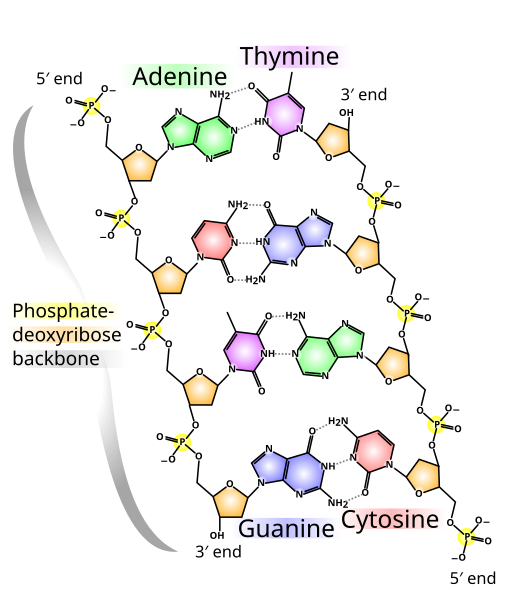
\includegraphics[width=0.5\textwidth]{512px-DNA_chemical_structure.svg.png}
    \caption[Chemical structure of DNA]{Chemical structure of DNA \cite{ball_DNA_structure}}
    \label{fig:dna-structure}
\end{figure}

\subsubsection{DNA methylation}
DNA is a sequence of one of four nucleotide bases: adenine (A), cytosine (C), guanine (G) and thymine (T), linked together by a deoxyribose sugar and phosphate backbone (see Diagram \ref{fig:dna-structure}). It is this sequence that provides genetic instructions. Like a human reading a book, strings of these bases are converted into information that tells cells how to function, called DNA transcription. Continuing the book analogy, a sentence of such instructions is called a gene, found in a chapter called a chromosome.

DNA methylation (DNAm) involves the addition of a methyl group (CH\(_3\)) to the 5-carbon position of cytosine nucleotides (see Diagram \ref{fig:cytosine-methylation}). This chemical modification to the cytosine makes it harder for transcription to occur, which can modulate, or even completely silence, gene expression. This is the most relevant and reproducible when a guanine is directly followed by a cytosine in the DNA sequence. Because of the phosphate connecting these bases, such a region is called a CpG site. CpG sites are the main form of DNAm that occurs in mammalian cells.

A biological sample used to assess DNAm will contain many thousands of copies of DNA. When measuring a CpG site for DNAm, the reported value is the percentage of DNA copies from the sample which are methylated. That is, a value between 0 (all DNA copies unmethylated) and 1 (all DNA copies methylated).

% At a high level, DNA is a sequence of letters that provide genetic instructions. Like a human reading a book, strings of these letters are converted into information that tells cells how to function. More precisely, these letters are one of four nucleotide bases: adenine (A), cytosine (C), guanine (G) and thymine (T). To form the sequence, these bases are attached to a deoxyribose sugar and connected by a phosphate molecule, called the sugar-phosphate backbone. Of relevance is the phosphate molecule, specifically for when a cytosine is directly followed by a guanine in the sequence. A phosphate bonding a cytosine and a guanine (called a CpG site) creates a chemical structure which allows methyl groups to attach. This process is an epigenetic modification called DNA methylation (DNAm). As a biomarker, we measure methylation at a CpG site as a float between 0 and 1, measuring the percentage of methylation at that site.

While the genetic sequence of DNA is stable, methylation is not. It is a dynamic state that depends on factors such as behaviours and environmental exposure \cite{greenberg2019diverse}. Exposure to a wide range of environmental factors including air pollutants \cite{martin2018environmental}, diet \cite{ma2020whole}, physical activity and even psychosocial stress \cite{opsasnick2024epigenome} have been shown to be associated with specific changes in DNAm. Moreover, sufficient lack of exposure to such factors can reverse such changes. As previously mentioned, DNAm affects the expression of genes. Methylation at a CpG site can silence the expression of the gene that site is located in, where more methylation at a site leads to stronger silencing. Moreover, DNAm is not random. There is strong correlation between methylation of specific sites with specific factors \cite{ewasatlas}. In the context of this work, smoking is strongly associated the methylation of cg05575921, found in the aryl hydrocarbon receptor
repressor (AHRR) gene \cite{reynolds2015dna}. With these points in mind, this means that DNA methylation of CpG sites can be used as a biomarker indicative of the factors that caused it, while also describing changes in cellular function. Therefore, DNAm is a biomarker not only useful for reporting on environmental exposures, but also predicting future health outcomes and risks. Examples of this include prediction of cardiovascular diseases \cite{cameron2023dna}, neurological diseases \cite{cells11213439}, type 2 diabetes \cite{cheng2023development}, pace of ageing \cite{10.7554/eLife.73420}, and cancer \cite{luo2020circulating}. Furthermore, DNAm is not self-reported, and therefore overcomes the biases associated with self-reported data.

Altogether, this motivates the use of DNAm data to develop methods for collecting smoking history of individuals. Work using such data is referred to as an epigenome-wide association study (EWAS).

\begin{figure}
    % \setcounter{figure}{\numexpr\value{figure}-1}
    \begin{subfigure}{0.49\textwidth}
        \centering
        \hspace*{11mm}
        \chemfig{*6(-\chembelow{N}{H}-(=O)-N=(-NH_2)-=)}
        \vspace{3mm}
        \caption{Cytosine}
    \end{subfigure}
    \begin{subfigure}{0.49\textwidth}
        \centering
        \chemfig{*6(-\chembelow{N}{H}-(=O)-N=(-NH_2)-(-H_3C)=)}
        \vspace{3mm}
        \caption{5-Methylcytosine}
    \end{subfigure}
    \caption[Methylation of cytosine]{Modification of cytosine into 5-methylcytosine caused by DNA methylation}
    \label{fig:cytosine-methylation}
\end{figure}

\subsubsection{DNAm arrays}
The human genome contains \(\sim\!28\) million CpG sites. This is often a computationally infeasible domain for a dataset, due to massive dataset sizes, processing requirements, and noise contained in the signal. Instead, most EWAS use a biologically relevant and informative subset of CpG sites, referred to as an array. There are two commonly chosen DNAm arrays used: Illumina 450k \cite{illumina2012methylation450} and Illumina EPIC \cite{illumina2015methylationepic}. 450k was the first array developed by Illumina, consisting of \num{485577} CpG sites chosen for their quality and usefulness. The EPIC array was developed as a successor, increasing the array size to \num{865859} CpG sites. However, only around \(>90\%\) of the sites were retained from 450k. This is something that needs to be considered when developing scores or screening tests from an EWAS if compatibility with multiple datasets or cohorts is of concern (see \ref{sec:pre-processing}). These arrays are compatible with DNA from multiple different cell types. Some examples include whole blood, purified cells and fresh-frozen tissue \cite{bhat2022data}. Moreover, the methylation signal can differ across different cell types \cite{huang2016epigenome}. This means selection of cell type can be an import factor when designing an EWAS. Typically, whole blood is used (specifically white blood cells, as red blood cells in humans do not carry a copy of the DNA) for its convenience \cite{houseman2015dna}.

% \vspace{1cm}
% \begin{itemize}
%     \item At a high level, DNA is a sequence of letters that provide genetic instructions
%     \item nucleotide bases (A, T, C, G) connected with a phosphate sugar backbone
%     \item Cs next to Gs create a chemical structure that allows methyl groups to attach: CpG site, = epigenetic modification
%     \item description of what the word epigenetics, "upon" genetics
%     \item While genetic sequence is stable, methylation is a dynamic state which depends on factors, enviroment etc.
%     \item The state of methylation can change/effect the expression of genes, where methylation = silencing.
%     \item Methylation isn't random, with strong correlation between methylation of specific CpG sites with specific factors
%     \item This means methylation status can be used as a biomarker for indicating and reporting on environmental exposures and report on health outcomes
%     \item Status of methylation sites can determine health outcomes, including cancer risk, CVD, diabetes, etc.
% \end{itemize}

% \subsubsection{DNAm Platforms}

% \begin{itemize}
%     \item Two types of DNAm platform, illumina 450k and illumina EPIC
%     \item \(\sim\)28 million CpG sites in the human genome, platforms choose specific sites to ranked
%     \item Cell type of sample matters, different cells with have different methylation. Typically whole blood is used, good general methylation signal.
% \end{itemize}

\subsection{Machine learning in epigenetics}
Broadly, machine learning algorithms are split into one of two tasks: regression or classification. The most significant distinction between these two tasks is the choice of supervised learning labels. Regression algorithms are trained against continuous, numeric scores, while classification algorithms are trained against discrete class labels. The choice of label in turn determines the output produced by the algorithm.
Machine learning has already seen use in many areas of clinical epigenetics. We begin with a review of some developed methods, addressing both classification and regression tasks.

\subsubsection{Applications} \label{sec:ml-examples}

Malta et al. \cite{malta2018machine} proposed a method for assessing oncogenic dedifferentiation (cells becoming cancerous). This approach seeks to model a "stemness index" which indicates how similar a cell is to stem cell - a trait found in cancerous cells. Of relevance is the developed epigenetic approach using one-class logistic regression. The training features consisted of 219 hyper-methylated CpG sites associated with stem cells. Training data only consisted of a single, positive, class: stem cells. The resulting model can then be fed non-stem cells to compare how similar they are to stem cells, i.e. cancerous cells.

Adorj\'an et al. \cite{adorjan2002tumour} proposed a method for using DNAm data to classify cancer tissues. CpG sites were ranked using a two sample t-test, and then fed into a support vector machine. Models were evaluated using the average of 50 runs of 8-fold cross-validation. The top two CpG sites could classify leukaemia from healthy cells with 84\% accuracy, while the top 60 sites achieve 94\% accuracy.

Dogan et al. \cite{dogan2018integrated} proposed a method for integrated genetic and epigenetic classification of coronary heart disease. The training dataset consisted of 1,545 individuals. An approach combining undersampling and ensemble learning \cite{liu2008exploratory} was used to address class imbalance, creating 8 training sub-datasets. Point biserial correlation and Pearson correlation were used for feature selection, resulting in 107,799 CpG sites for training. These features were ranked using ROC-AUC. Random Forest classifiers were then trained on the 8 training sub-datasets, with majority voting used for ensembling. Hyperparameters were tuned using 10-fold cross-validation. The final model used 4 CpG sites, two genetic variables, age and sex. This achieved an accuracy, sensitivity and specificity of 78\%, 0.75 and 0.80, respectively.

Adeoye et al. \cite{adeoye2022machine} proposed a method for using saliva samples to detect oral cancer. This study aimed to propose an alternative to tissue biopsy, which can be invasive and prone to false-negatives. Training data consisted of saliva samples of 33 randomly selected patients with oral cancer. Eight machine learning models were compared (RBF kernel, SVMs, AdaBoost, kNNs, random forest, decision trees, ExtraTrees, and gradient boosting machines) alongside three feature selection techniques (ANOVA, MRMR and LASSO). The SVM was the best performing model, with a recall, specificity and precision of 0.94, 0.93 and 0.94, respectively, while LASSO was the most robust feature selection technique across all machine learning models.

Cheng et al. \cite{cheng2023development} proposed a method for predicting the risk of developing type 2 diabetes within the next 10 years. Training data consisted of 374 cases and \num{9461} controls, for a total of \num{9835} individuals. Several penalised regression models were trained, including Cox proportional-hazards with LASSO regularisation, random survival forests, and survival bayesian additive regression trees. Evaluation compared models using only traditional risk factors against models that included DNAm factors. All models showed incremental gains in performance with the addition of DNAm factors, with an increase in ROC-AUC values. The best performing model was the Cox proportional-hazards with LASSO regularisation, which reported an ROC-AUC of 0.872.

\subsection{Smoking algorithms}
In the context of smoking, the two most significant machine learning epigenetic scores use Elastic Net regression.

\subsubsection{Elastic Net regression} \label{sec:lin-elastic-net}
Elastic Net \cite{zou2005regularization} is a regularised form of linear regression that includes two additional penalty terms.
Given \(n\) examples, \(p\) features with data \(x \in \mathbb{R}^{n \times (p + 1)}\) and corresponding ground-truth \(y \in \mathbb{R}^n\), we find coefficients \(\beta \in \mathbb{R}^{p + 1}\) that produces an output:
\[\hat{y} = x \beta \in \mathbb{R}^{p + 1}\]
and minimises the function:
\begin{equation} \equationname{Elastic Net linear regression} \label{eqn:lin_elastic_net}
    \mathcal{L}(y, \hat{y}, \beta) = ||y - \hat{y}||_2^2 + \alpha\lambda||\beta||_1 + \alpha\frac{1 - \lambda}{2}||\beta||_2^2
\end{equation}
where
\[||\beta||_1 = \sum_{i=1}^{p} |\beta_i|\]
and:
\[||\beta||_2 = \sqrt{\sum_{i=1}^{p} \beta_i^2}\]

We can see this is simply mean-squared error, with the \(L_1\)-norm and \(L_2\)-norm included as penalisation terms on \(\beta\). The two hyperparameters \(\alpha\) and \(\lambda\) control the regularisation strength and ratio between \(L_1\)-norm and \(L_2\)-norms, respectively. Elastic Net is a combination of two other forms of regularised linear regression: lasso \cite{tibshirani1996regression} and ridge \cite{hoerl1970ridge} regression. The two mathematical regularisation terms have interpretable effects on the convergence of \(\beta\). Gradient updates for \(||\beta||_1\) are uniform for all non-zero values of \(\beta_i\), which typically results in most \(\beta_i\) set to zero, with some having large values. This is referred to as a sparse solution. Gradient updates for \(||\beta||_2^2\) are large for large \(\beta_i\), and small for small \(\beta_i\), which typically results in all \(\beta_i\) having similar values. This is referred to as shrinkage. Together, this results in Elastic Net models promoting the grouping effect, where strongly related features are all included or excluded together. This grouping effect is particularly useful when \(p > n\), as it provides better feature selection than lasso \cite{zou2005regularization}. Because of this, Elastic Net sees wide use in epigenetics, with biological age clocks being one area of particular use \cite{teschendorff2025epigenetic}.

\subsubsection{DNAmPACKYRS} \label{sec:dnampackyrs}
Lu et al. \cite{lu2019dna} proposed DNAmPACKYRS as a DNAm based score for calculating smoking pack-years. This score was originally developed as surrogate biomarker for use in the DNAm GrimAge \cite{lu2019dna} and DNAm GrimAge v2 epigenetic clocks \cite{lu2022dna}. DNAm GrimAge is a regression model for estimating mortality risk. The DNAm GrimAge score is calculated using the covariates sex, age, 7 surrogate biomarkers of plasma proteins, and of relevance, a surrogate biomarker for smoking pack-years: DNAmPACKYRS. Elastic Net regression was used to train both DNAm GrimAge and the surrogate biomarkers of plasma proteins and pack-years. Training data consisted of 1731 individuals from the Framingham Heart Study (FHS) dataset \cite{doi:10.2105/AJPH.41.3.279}. Individuals from this dataset had a mean age of 66 years. 54\% of individuals were female, leaving 45\% as male. The intersection of sites available on Illumina 450k and Illumina EPIC were chosen as the available CpG sites for training. This was to ensure compatibility and future-proofing with new datasets. A total of \num{450161} CpG sites were available. 10-fold cross-validation was used for hyperparameter tuning the regularisation strength of the Elastic Net model. This resulted in the DNAmPACKYRS score which used 172 CpG sites.

As surrogate biomarker for lifespan, DNAmPACKYRS performs better than self-reported pack-years. Firstly, DNAmPACKYRS can be used to predict lifespan in never-smokers \cite{lu2019dna}, whereas self-reported pack-years cannot (all self-reported values would be 0). Additionally, DNAmPACKYRS is a more significant predictor of lifespan than self-reported pack-years. Across 4 out of 5 datasets DNAmPACKYRS had a smaller Cox regression p-values when compared to self-reported pack-years \cite{lu2019dna}. Since DNAmPACKYRS is only evaluated as a surrogate biomarker in the GrimAge paper, there is no reporting on its performance of predicting smoking status. However, this can be done independently (see \ref{sec:model-comparisons}). When performed, we can see that DNAmPACKYRS achieves ROC-AUCs of 0.991, 0.915 and 0.798 for separating never- vs current-, ex- vs current- and never- vs ex-smokers, respectively.
% \(8.10\mathrm{e}{-23}\) vs \(1.12\mathrm{e}{-11}\), \(8.51\mathrm{e}{-5}\) vs \(2.13\mathrm{e}{-3}\), \(7.17\mathrm{e}{-12}\) vs \(7.03\mathrm{e}{-12}\), \(2.1\mathrm{e}{-19}\) vs \(6.4\mathrm{e}{-19}\), and \(5.33\mathrm{e}{-4}\) vs \(1.78\mathrm{e}{-1}\), respectively. 

There are some limitations with the DNAmPACKYRS score. While the score achieves excellent performance separating current-smokers from the other smokers, performance separating never-smokers and ex-smokers is modest. Additionally, the choice of self-reported pack-years as a regression label introduces a source of inaccuracy, discussed below (see \ref{sec:mcigarette}).

% Notes for DNAmPACKYRS/mCigarette:
% \begin{itemize}
%     \item dataset/cohort/demographic
%     \item algorithms
%     \item result/stat it produces
%     \item limitations
% \end{itemize}

\subsubsection{mCigarette} \label{sec:mcigarette}
Chybowska et al. \cite{chybowska2025blood} proposed mCigarette as a DNAm based score for calculating pack-years. This score was part of the very recent (2025) study comparing brain- and blood-based DNAm associated with smoking. This worked aimed to overcome the limitations of self-reported smoking data, as well as the modest performance of separating never-smokers from ex-smokers of previous studies. Several techniques were employed, including high resolution approaches involving \(\sim \! 20\) million CpG sites. The most relevant method is the developed smoking biomarker: mCigarette. Similar to DNAmPACKYRS, this is a methylation based score for smoking pack-years trained with Elastic Net Regression. Training data consisted of \num{17865} individuals from the Generation Scotland (GS) dataset \cite{smith2006generation}, which was developed on the Illumina EPIC array. Individuals from this dataset had a mean age of 47.6 years. 59.1\% of the individuals were female. CpG sites were filtered based on statistical association with tobacco use at a false discovery rate (FDR) \(< 0.05\), resulting in \num{18760} CpG sites per individuals. This filtering was run in a dataset separate to the training dataset, using the Illumina 450k array. Note that this limits training features those CpG sites found on both the 450k and EPIC arrays. Elastic Net regression was then used to train the mCigarette score. Hyperparameters were tuned using 10-fold cross-validation, which set \(\alpha = 0.012577\), while \(\lambda\) was fixed at \(0.5\). This resulted in a model using \num{1255} CpG sites. As a result, mCigarette achieved improved performance compared to previous scores. In an independent validation cohort, mCigarette achieved ROC-AUCs of 0.98, 0.90 and 0.85 for current- vs never-, current- vs ex- and never- vs ex-smokers, respectively.

% Two ex-smokers (both 70 years of age) with the same pack year value but very different smoking-related chronic disease risk.  Person A gave up smoking 1year ago but had smoked half a pack a day for the last 40 years (20 pack years), Person B smoked 2 packs a day from 15-25 years age (20 pack years) but hasn’t smoked in 45 years.  Chronic disease (eg. Lung cancer and heart disease) risk is much higher in person A than B.  Moreover, we would expect very different smoking related DNA methylation values between the two people.

There are limitations associated with the mCigarette score. The choice of smoking pack-years may be inaccurate as a training label, due to the potential to identified two individuals with significantly different smoking exposures as similar. As an example, consider two ex-smokers both of 70 years of age. Individual A gave up smoking 1 year ago, but smoked half a pack of cigarettes per day for 40 years prior, which equates to 20 pack-years. Individual B smoked 2 packs of cigarettes per day from ages 15 to 25 but has quit since, which also equates to 20 pack-years. Both individuals have the same smoking pack-years score, but different lengths of cessation (1 year vs 45 years). This is problematic, as risk of chronic disease (e.g. lung cancer and cardiovascular disease) would be expected to be much higher in individual A than individual B, as duration of smoking carries greater risk than intensity of smoking \cite{remen2018risk, flanders2003lung, lubin2006cigarette, doll1978cigarette}. Moreover, we would expect different smoking-related methylation signals for the two individuals. Thus, individuals with less intense but longer duration of smoking exposure may have underestimated smoking exposure by such a model. Therefore, smoking pack-years is an inaccurate and biased choice of training label, as it assigns equal importance to smoking duration and smoking intensity \cite{potter2024pack}. As mentioned above, this limitation is also associated with the DNAmPACKYRS score, which also used smoking pack-years for training labels.

% \begin{itemize}
%     \item[\checkmark] (?) seeking to address not being able to differentiate never- smokers and ex-smokers
%     \item[\checkmark] 17865 individuals
%     \item[\checkmark] filtered CpG sites to FDR \(< 0.05\) \((n = 18760)\)
%     \item[\checkmark] elastic net regression
%     \item[\checkmark] 10-fold cross-validation, \(\lambda = 0.012577\)
%     \item[\checkmark] 1255 CpG sites used in model
%     \item[\checkmark] in validation cohort, AUCs of Current- vs Never-: 0.98, Current- vs Former: 0.90, Former vs Never-: 0.85
%     \item limitation 2: choice of ground truth (sr pack-years) is potentially confusing for the model
% \end{itemize}

\subsection{Aim of this work}

As discussed, there are limitations associated with using smoking pack-years as a training label, namely, not accounting for the length of smoking cessation. This could be addressed by adjusting smoking pack-year values for the length of smoking cessation. However, this would require the use of additional self-reported data, which could also introduce further bias. As an alternative to smoking pack-years, self-reported smoking status (current-, ex- or never-smoker) is a more consistent measure of lifetime smoking exposure. In contrast to previous work which uses smoking pack-years, we propose Elastic Net Smoking-Status (ENSS) as a method which uses smoking-status as a training label for supervised machine learning.  Since smoking-status is a discrete variable (rather than continuous like smoking pack-years), this required reframing the modelling of smoking history as a classification task rather than a regression task. While current methods for predicting smoking history perform well separating current-smokers from other smokers, performance separating never-smokers from ex-smokers is modest. Because of the described limitations of smoking pack-years, the change to smoking-status in our proposed method aimed to achieve better class separation between never-smokers and ex-smokers.

% mention that SRSS is more reliable than pack-years
% srss abbreviation 

\section{Method}

\subsection{Algorithm} \label{sec:algorithm}
We begin by transforming Elastic Net from a regression problem into a classification problem. In the binary classification case, this is achieved by a straightforward modification to the loss function, replacing the mean-square error term with a binary-cross entropy error term, alongside transforming the linear prediction into probabilities via the sigmoid function. However, in the multi-class classification case the modification is more complex, and also affects the regularisation terms. We modify the algorithm seen in \ref{sec:lin-elastic-net} as follows:

Given \(n\) examples, \(p\) features, \(K\) classes with data \(x \in \mathbb{R}^{n \times (p + 1)}\) and corresponding ground-truth \(y \in \mathbb{R}^{n \times K}\) (as one-hot encoded vectors), we find coefficients \(\beta \in \mathbb{R}^{K \times (p + 1)}\) that produces logits:
\[z = x \beta^\mathsf{T} \in \mathbb{R}^{n \times K}\]
We transform a row of logits into probabilities with the softmax function:
\[\hat{y_i} = \softmax(z_i) \in \mathbb{R}^{n \times K}\]
where:
\[\softmax(t_1,\hdots , t_k) =
    \begin{bmatrix}
        \frac{\exp(t_1)}{\sum_{j=1}^{K} \exp(t_j)}
        \hdots
        \frac{\exp(t_k)}{\sum_{j=1}^{K} \exp(t_j)}
    \end{bmatrix}
\]
The loss function then becomes:
\begin{equation} \equationname{Elastic Net logistic regression} \label{eqn:mc_log_elastic_net}
    \mathcal{L}(y, \hat{y}, \beta) = -\frac{1}{n}\sum_{i=1}^{n} y_i \cdot \log(\hat{y_i}) + \alpha\sum_{k=1}^{K}(\lambda||\beta_k||_1 + (1 - \lambda)||\beta_k||_2^2)
\end{equation}
where the \(L_1\)-norm and \(L_2\)-norm are as before.

The output of this model \(\hat{y}\) is matrix of \(K\) probability predictions, one for each class, for \(n\) different examples. For each example, the softmax function ensures the \(K\) predicted probabilities from these logits will sum to 1. To make a prediction for the \(i^\text{th}\) example, the model chooses the class with the largest probability: \(\argmax(\hat{y_i})\). Alternatively, this model can be thought of as training an ensemble of \(K\) individual logistic regression predictors. Each of \(K\) rows of \(\beta\) is a class-specific linear predictor that produces logits for predicting a single class. Regularisation terms work as before, but are now regularising coefficients per-class-specific linear predictor, rather than regularising all coefficients in the model together.

\subsection{Datasets}
This work used two datasets, a discovery cohort and an independent test cohort.

\subsubsection{Cohort 1: Discovery}
Cohort 1 contained DNAm data for 943 individuals. Across these individuals, 100\% were male, and there was a mean age of 72 years. Data was collected using the Illumina 450k array, which measured the methylation of \num{449521} CpG sites using the white blood cells found in whole blood samples. To ensure model compatibility with independent datasets, available CpG sites were restricted to those found on both the Illumina 450k and EPIC arrays. This reduced available CpG sites by \(\sim\!10\%\). Note that this practice was consistent with the methods seen in previous work (see \ref{sec:dnampackyrs} and \ref{sec:mcigarette}). Alongside epigenetic data, age, sex, self-reported pack-years and self-reported smoking-status were also recorded. Of the 943 individuals, 235 were never-smokers, 599 were ex-smokers and 109 were current-smokers. 90\% of this cohort was used as the model's training dataset, while the remaining 10\% was reserved as a hold-out test dataset to evaluate model performance. This split was done in a stratified manner, which preserved the class balance from the original cohort.

% \begin{itemize}
%     \item[\checkmark] Illumina 450k
%     \item[\checkmark] all males
%     \item[\checkmark] mean age 72
%     \item[\checkmark] 235 never- smokers, 599 ex smokers, 109 current- smokers
%     \item 90/10 train/test split
%           \begin{itemize}
%               \item 211 never- smokers, 539 ex smokers, 98 current- smokers in training split
%               \item 24 never- smokers, 60 ex smokers, 11 current- smokers in test split
%           \end{itemize}
%     \item[\checkmark] \num{449521} CpG sites
%     \item[\checkmark] white blood cells from whole blood
% \end{itemize}

\subsubsection{Cohort 2: Evaluation}
Cohort 2 contained DNAm data for 984 individuals. Across these individuals 67\% were male, and there was a mean age of 68 years. Data was collected using the Illumina EPIC array, which measured \num{865,859} CpG sites using the white blood cells found in whole blood samples. Because the model was trained on a dataset using the 450k array, the available sites in this evaluation dataset were restricted to those found on both Illumina 450k and EPIC. This reduced available CpG sites by \(\sim\!50\%\). Alongside epigenetic data, age, sex, self-reported pack-years and self-reported smoking-status were also recorded. Of the 984 individuals, 403 were never-smokers, 476 were ex-smokers and 105 were current-smokers. In addition to independently testing ENSS' performance, this dataset was used to compare ENSS to the externally-derived, existing gold standard models.

\subsubsection{Choice of discovery and evaluation cohorts}
This approach of using two independent datasets to train and evaluate a model is not conventional in machine learning. Instead, all available data is split in training, validation and testing sets. However, independent testing data is common practice in clinical research. Not only does this evaluate overfitting, it also evaluates generalisability across populations and ascertainment bias, both relevant challenges when developing a clinical test. Because of the multidisciplinary nature of this project, a combination of both approaches was used. This then required deciding which cohort would provide training data, and which would be used for evaluation. Cohort 1 was selected for training as it contained only males. Given that sex is a likely confounder of lifetime smoking exposure (males tend to smoke more than females \cite{WHO2021Tobacco, higgins2015literature}), Cohort 1 was deemed to be a less-confounded dataset.

Summaries of the datasets used in this study can be seen in Table \ref{table:dataset-compare-internal}.

% \begin{itemize}
%     \item Illumina EPIC
%     \item 67\% of individuals were male (n=658) (female n=326)
%     \item mean age 68
%     \item 403 never- smokers, 476 ex smokers, 105 current- smokers
%     \item \num{449521} CpG sites (intersection with 450k)
%     \item white blood cells from whole blood
% \end{itemize}

\begin{table}
    \caption{Training and testing dataset comparisons} \label{table:dataset-compare-internal}
    \begin{tabularx}{\textwidth}{X >{\raggedleft\arraybackslash}X >{\raggedleft\arraybackslash}X >{\raggedleft\arraybackslash}X}
        \toprule
        \textbf{Measure}    & \textbf{Cohort 1 - Train}     & \textbf{Cohort 1 - Test}     & \textbf{Cohort 2}             \\
        % \addlinespace
        \midrule
        \multicolumn{4}{c}{\textbf{Class balance}}                                                                         \\
        \midrule
        Num. individuals    & \num{848}                     & \num{95}                     & \num{984}                     \\
        \addlinespace
        Never-Smokers       & \num{211} (\SI{25}{\percent}) & \num{24} (\SI{25}{\percent}) & \num{403} (\SI{41}{\percent}) \\
        \addlinespace
        Ex-Smokers          & \num{539} (\SI{63}{\percent}) & \num{60} (\SI{63}{\percent}) & \num{476} (\SI{48}{\percent}) \\
        \addlinespace
        Current-Smokers     & \num{98} (\SI{12}{\percent})  & \num{11} (\SI{12}{\percent}) & \num{105} (\SI{11}{\percent}) \\
        % \addlinespace
        \midrule
        \multicolumn{4}{c}{\textbf{Cohort distribution}}                                                                   \\
        \midrule
        Percentage male     & \SI{100}{\percent}            & \SI{100}{\percent}           & \SI{67}{\percent}             \\
        Mean age            & \num{72}                      & \num{71.5}                   & \num{68}                      \\
        % \addlinespace
        \midrule
        \multicolumn{4}{c}{\textbf{Num. CpG sites}}                                                                        \\
        \midrule
        Raw Illumina array  & \num{485577}                  & \num{485577}                 & \num{865859}                  \\
        Post-intersection   & \num{449521}                  & \num{449521}                 & \num{449521}                  \\
        Percentage retained & \SI{93}{\percent}             & \SI{93}{\percent}            & \SI{52}{\percent}             \\
        \bottomrule
    \end{tabularx}
\end{table}

\subsection{Hardware and software}
Pre-processing, training and the production of results were run on an M2 MacBook Air. This device had an Apple M2 processor with 8 CPU cores and 8 GPU cores, 16GB of unified memory, and the macOS Sonoma version 14.2 operating system. Code implementations were written in Python (version 3.9.10), using the scikit-learn (version 1.6.0) \cite{scikit-learn}, SciPy (version 1.13.1) \cite{SciPy} and NumPy (version 1.26.4) \cite{harris2020array} packages.

\subsection{Pre-processing} \label{sec:pre-processing}
Both datasets required preparation before training. Raw Illumina array text files came in a format suitable for an EWAS, but not machine learning. Preparation steps included conversion into comma separated value format, merging and formatting of headers, transposing whole files, and splitting into separate labels and data files. Because of the large file size (\(\sim\!3.5\) GB per dataset), not all operations could be run in-memory. To address this, the pre-processing pipeline made multiple writes to the disk, requiring \(\sim\!10\) GB of storage per dataset (including the initial dataset file). These memory limitations were most noticeable when transposing whole EWAS files, requiring a package to process files in chunks \cite{transposecsv}.

Available CpG sites for training were filtered in two different ways. Firstly, as previously mentioned, both datasets were filtered to the intersection of CpG sites available on both the 450k and EPIC arrays, to ensure compatibility. Secondly, training data required pre-training feature selection. High dimensional data is a well observed technical challenge for machine learning \cite{cai2018feature}. From a technical perspective, early experimentation showed model training not converging with an input space of the order of \num{10000} features, despite supervised feature selection being built into the model (see Equation \ref{eqn:mc_log_elastic_net}). However, an input space of the order of \num{1000} or \num{100} features converged adequately. The concept of sample complexity (the number of examples needed for a model to achieve sufficient accuracy) is well recognised \cite{blum1997selection}, suggesting additional feature selection, alongside the regularisation built into the model, was required for the given sample size. From a practical perspective, a test which uses fewer features is more cost-effective and interpretable, hence more likely to be translatable to clinical applications. Therefore, developing a model which achieves sufficient accuracy with the fewest features possible is desirable. To implement this feature selection, we used the Kruskal-Wallis test by ranks.

\subsubsection{Feature selection: Kruskal-Wallis test} \label{sec:feature-selection}
The Kruskal-Wallis test by ranks \cite{Kruskal1952UseOR} is a non-parametric statistical test that identifies if there are statistically significant differences between the distributions of observations for two or more samples. In the context of this work, the test was run per CpG site, where the samples are classes of smoking status (current-, ex-, never-smokers) and observations are DNAm values for that site. Applying this test to the training dataset identifies the CpG sites which are the most differentially methylated across all three classes of smoking status. More commonly used statistical tests are the one-way ANOVA \cite{fisher1921probable} or Mann-Whitney U \cite{mann1947test} tests. One-way ANOVA is a parametric test for two or more samples, while Mann-Whitney is a non-parametric test for exactly two samples. A parametric test assumes the samples are drawn from populations which are normally distributed, and there is no evidence to make this assumption for DNAm data. A goal of this work was to improve class separation between all three classes, motivating the use of a test on two or more samples, rather than running a test on exactly two samples pair-wise three times. For these reasons, these tests were rejected in favour of the Kruskal-Wallis test. In fact, Kruskal-Wallis is the non-parametric equivalent of one-way ANOVA, and extension to more than two samples of Mann-Whitney, making this a natural choice.

To run the test, first all observations are ranked (sorted in ascending order, with correction for ties). The test statistic is then given by:
\begin{equation} \equationname{Kruskal-Wallis test by ranks}
    H = \frac{12}{N(N + 1)}\sum_{i=1}^{C}\frac{R_i^2}{n_i} - 3(N + 1)
\end{equation}
where \(C\) is the number of samples, \(n_i\) is the number of observations in the \(i^\text{th}\) sample, \(N = \sum n_i\) is the number of observations in all samples, and \(R_i\) is the sum of the ranks in the \(i^\text{th}\) sample. The null-hypothesis is the distributions of all samples are the same. A large value of \(H\) is indicative of rejecting the null-hypothesis. Moreover, approximating the distribution of the \(H\) statistic as a chi-squared distribution allows the calculation of \(p\)-values. However, because the test was run hundreds of thousands of times, there is an increased chance at least one test was deemed significant (i.e. a false positive) due to random chance. To control the false discovery rate (FDR), we used Benjamini-Hochberg correction \cite{benjamini1995controlling} to turn \(p\)-values into false discovery corrected \(q\)-values. To achieve feature selection, we retained all CpG sites with a \(q\text{-value} < 0.05\). Implementations of the Kruskal-Wallis test and Benjamini-Hochberg correction are provided by SciPy, via the \verb|scipy.stats.kruskal| and \verb|scipy.stats.false_discovery_control| functions.

% \vspace{1cm}
% \textbf{Discussion points for Pre-Processing:}
% \begin{itemize}
%     \item[\checkmark] structure wrong to read off a full set of features for a given individual
%     \item[\checkmark] required transposing, memory heavy operation
%     \item[\checkmark] Why we need feature selection (brief, I have a couple sources for it, benchmarks of model being able to train (check notebook), and the cost associated with lots of CpG sites, explainability for a clinical test (if you can do the same thing in less sites, you want to)) \textbf{this last point is important as it justifies all the results/discussion about the CpG sites used}
%     \item[\checkmark] Kruskal Wallis chosen over Mann Whitney U to try to achieve better class separation
%     \item[\checkmark] Kruskal wallis chosen over one-way ANOVA as no strong assumptions are made about the distribution from which the samples are drawn
%     \item we make the assumption that each CpG site is independent, not actually true
%     \item[\checkmark] using q-values over p-values, false discovery correction.
% \end{itemize}

\subsection{Training} \label{sec:training}

The \num{3122} sites identified by the Kruskal-Wallis test were then utilised in machine learning training. Using the 848 individuals from the cohort 1 training set, DNAm values from these sites were used to train a multi-class Elastic Net logistic regression model. The implementation of this model was provided by scikit-learn, via the \verb|linear_model.LogisticRegression| class. This model used the Elastic Net penalty and SAGA solver, as this is the only solver compatible with Elastic Net regularisation. However, this does make the model stochastic. Additionally, the model used balanced class weights. Because of the class imbalance in the training dataset (see Table \ref{table:dataset-compare-internal}) the model was performing poorly when classifying never-smokers and current-smokers. By using balanced class weights, gradient updates are scaled inversely-proportional to the frequency of the given class. While this fixed the misclassification issues, it also can increase the chance of overfitting if the class balance present in the training sample is not representative of the true population.

Two of the hyperparameters required tuning: regularisation strength (\(\alpha\)) and \(L_1\) ratio (\(\lambda\)). Values for these were determined using a combination of k-fold cross-validation and grid search. In particular, the training dataset was split into 10 stratified folds for use in cross-validation. A choice of \(k=10\) was used to ensure each run in the cross-validation loop contained sufficient training data, because of the relatively low training dataset size. Folds were chosen to be stratified to because of the class imbalance. Cross-validation was used instead of a typical validation hold-out set in order to preserve the size of the training dataset. A grid search was used to evaluate the different combinations of hyperparameters. \(F_1\)-macro was selected as the scoring function to evaluate each fit, as each class is equally represented in the score, in spite of class imbalance. Outputs of cross-validation included the mean and standard deviation of \(F_1\)-macro scores across the 10 folds per fit. These were then used to calculate 95\% confidence intervals (see Figure \ref{fig:cross-validation}). Because the majority of hyperparameter choices had overlapping 95\% confidence intervals, they were deemed to not be statistically different. Therefore, hyperparameters were selected to increase regularisation strength and minimise the number of features used in the final model. This resulted in a choice of \(\alpha = 0.2\) and \(\lambda = 0.85\), which were used to retrain the Elastic Net model on the entire training dataset. Henceforth, we refer to this trained model as Elastic Net Smoking-Status (ENSS). Implementations of cross-validation and grid search were provided by scikit-learn, via the \verb|sklearn.model_selection.StratifiedKFold| and \verb|sklearn.model_selection.GridSearchCV| classes.

\begin{figure}
    \centering
    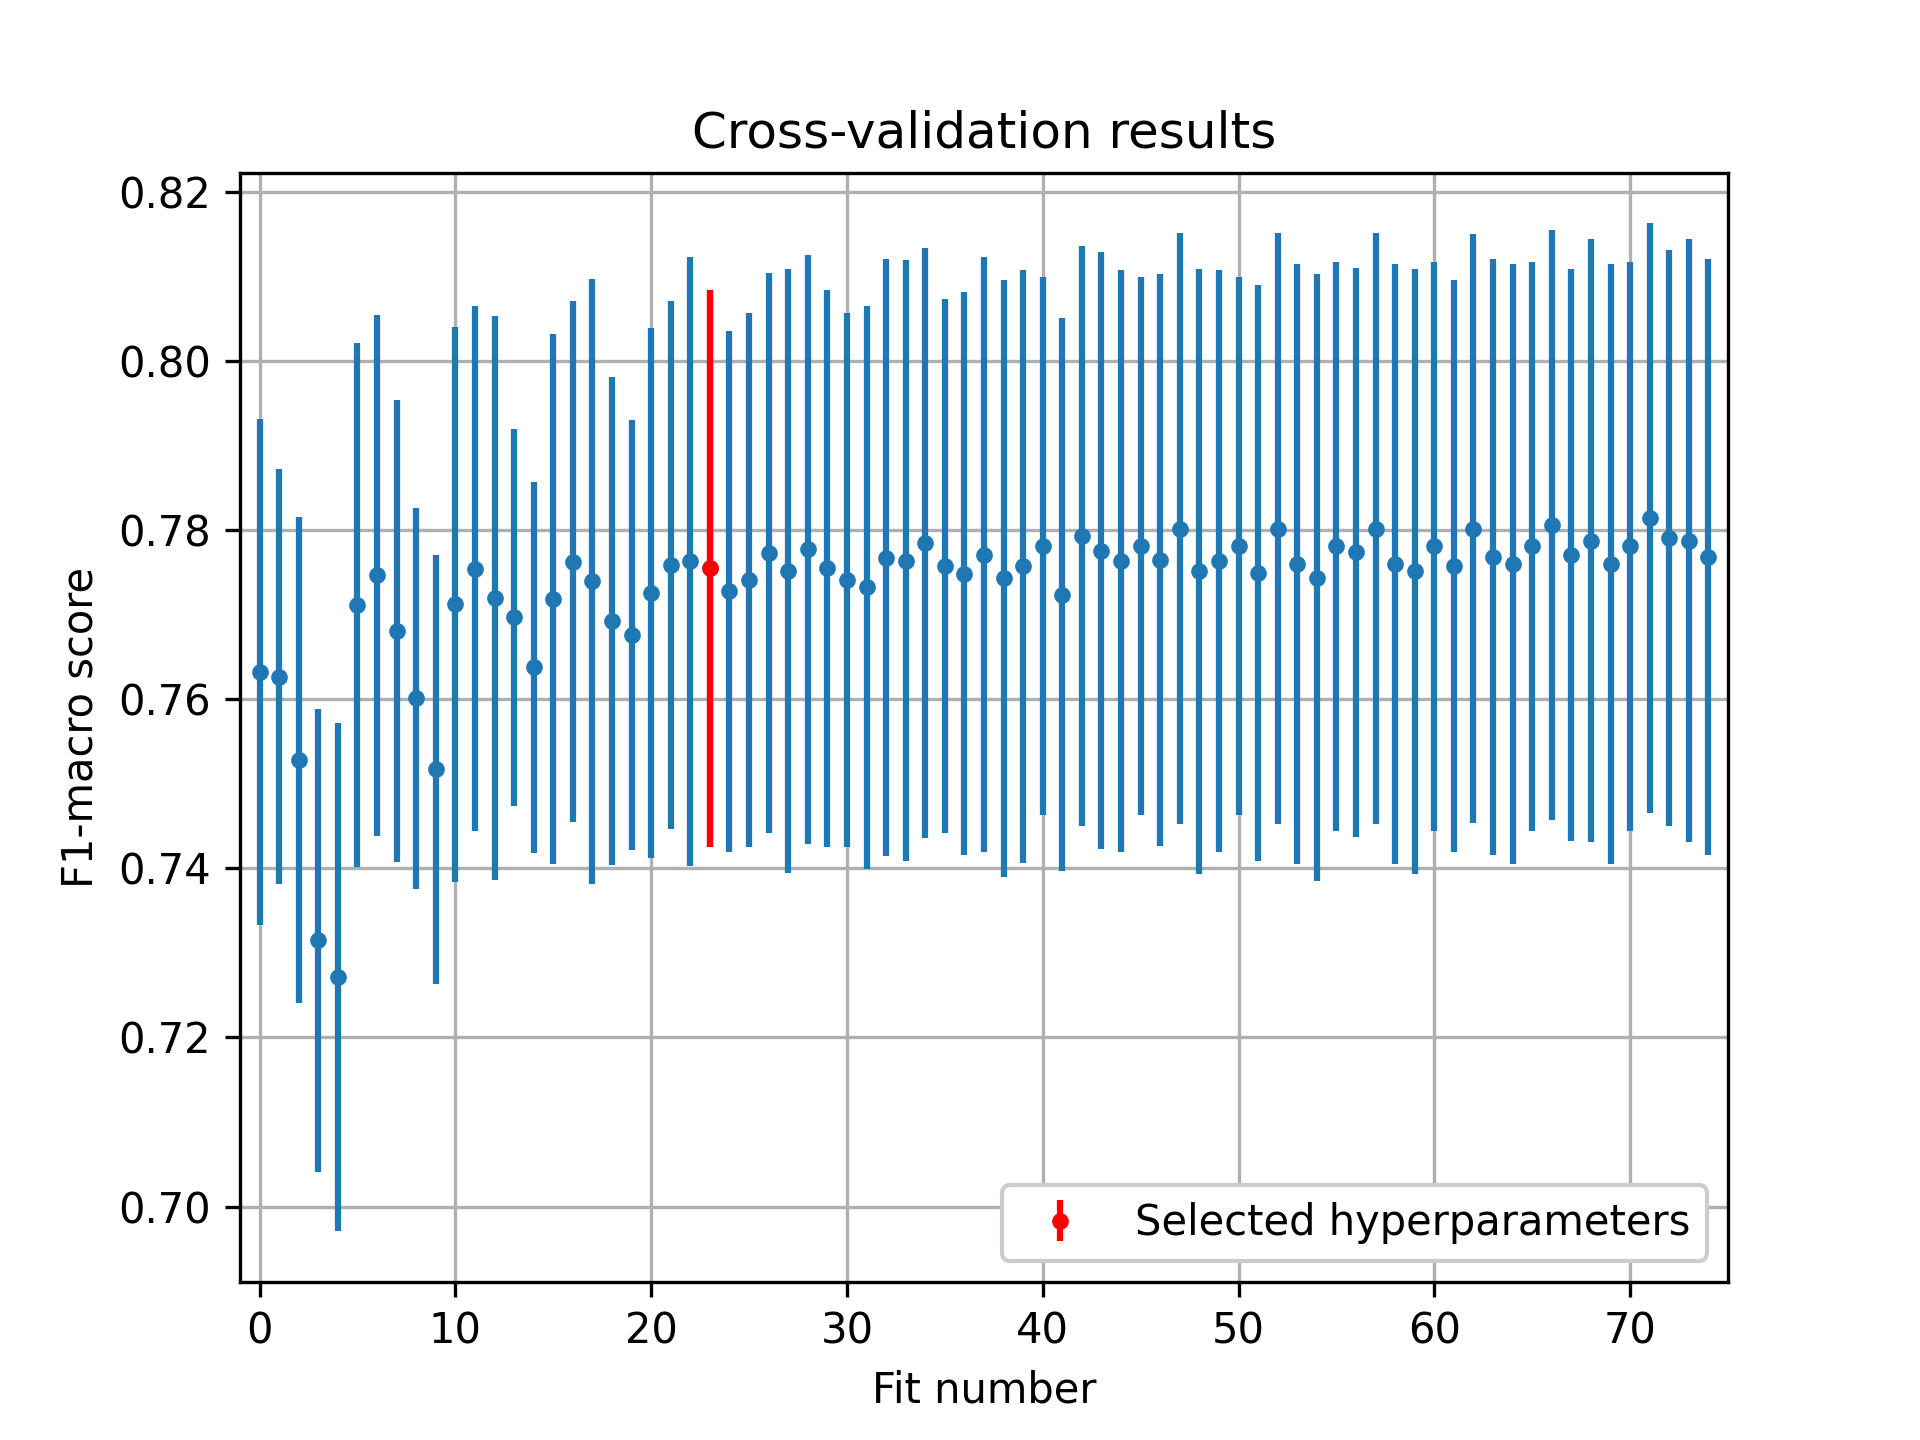
\includegraphics[width=0.8\linewidth]{cross_validation.png}
    \caption[Cross-validation scores per fit]{\(F_1\)-macro scores for each fit during cross-validation. Error bars indicate 95\% confidence intervals. Because of the overlapping confidence intervals, the choices of hyperparameters were not deemed to be statistically different.}
    \label{fig:cross-validation}
\end{figure}

Additionally, a linear regression Elastic Net model was trained to benchmark against, using the same algorithm seen in DNAmPACKYRS and mCigarette (see Equation \ref{eqn:lin_elastic_net}). This model used the same choice of hyperparameters as the logistic regression model, and used self-reported pack-years as a training label. The implementation of this model was provided by scikit-learn, via the \verb|linear_model.ElasticNet| class.

\section{Results} \label{sec:results}

\subsection{Site reduction from feature selection and regularisation}
As discussed in the method (\ref{sec:feature-selection}), the Kruskal-Wallis test was used to select CpG sites as a feature selection step. The test was run independently on the \num{485577} CpG sites common to the 450k and EPIC arrays, using the observations (DNAm values) from cohort 1. After controlling for FDR, \num{3122} CpG sites remained with a \(q\text{-value} < 0.05\).

From the \num{3122} sites identified by the Kruskal-Wallis test, the Elastic Net logistic regression model selected \num{2381} different sites used in predicting smoking status. These \num{2381} sites consisted of three sets of CpG sites, where each set contained the sites used to predict the probabilities for never-, ex- and current-smokers, respectively.
The intersections of these sets can be seen in Figure \ref{fig:cpg-intersection-internal}. While \num{2381} total sites were used for the entire model, only \num{520} were common to predicting all 3 classes of smoking status. While each class-specific predictor regularised to a similar number of CpG sites (\num{1653} for never, \num{1627} for ex and \num{1514} for current), there were \num{1373} sites used in the prediction of exactly two of the three classes, and \num{488} sites used in the prediction of exactly one class. The limited overlap between the features used in each class-specific predictor was unsurprising, as the \(L_1\)-norm is applied per class (see Equation \ref{eqn:mc_log_elastic_net}) rather than across all parameters used in the model. However, this property is not desirable, as it led to a larger number of CpG sites used in the entire model.

\begin{figure}[h]
    \centering
    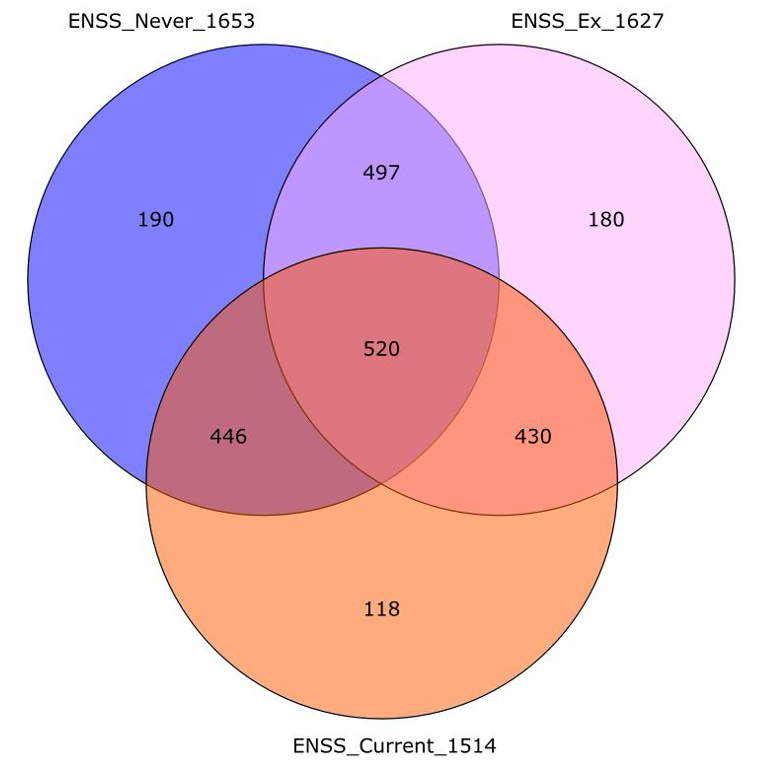
\includegraphics[width=0.7\linewidth]{venn_diagrams/predictor_intersect_placeholder.png}
    \caption[Model CpG site intersections]{Intersection of CpG sites used per class-specific predictor}
    \label{fig:cpg-intersection-internal}
\end{figure}

\subsection{Evaluation metrics}
The potential utility of a smoking model lies in its ability to differentiate pairs of classes (i.e. never- vs current-, ex- vs current- and never- vs ex-). Moreover, the multi-class model can be thought of as an ensemble of three classifiers that each predict the probability of a different class (see \ref{sec:algorithm}). Therefore, the model's ability to separate classes was evaluated using receiver operating characteristic (ROC) curves, using a one vs one (OvO) strategy to compare pairs of classes \cite{scikit-learn-roc-example}. Two types of ROC curves were evaluated. First, ROC curves of the probabilities for each of the class-specific predictors were evaluated. These show a single set of coefficients ability to separate two classes. Subsequently, macro-averaging \cite{scikit-learn-roc-example} was used to aggregate the outputs of both relevant class-specific predictors, which generated a single ROC curve used for evaluating OvO class separation of the entire model.
The red points on ROC curves indicate the optimal threshold for separation, calculated using Youden's index \cite{youden1950index}. Area under the curve (AUC) was used as an aggregated score for how well the model separated the two classes, reflecting both sensitivity (true positive rate) and specificity (true negative rate). The rubric used throughout this work for evaluating AUCs can be seen in Table \ref{table:auc-eval}.

\begin{table}[tb]
    \caption{AUC evaluation rubric} \label{table:auc-eval}
    \begin{tabularx}{\textwidth}{l l X}
        \toprule
        \textbf{AUC range} & \textbf{Discrimination ability} & \textbf{Usefulness}                                                              \\
        \midrule
        0.9 to 1.0         & Excellent                       & Near perfect separation of the two groups, with 1.0 being perfect discrimination \\[1em]
        \addlinespace
        0.8 to 0.9         & Good                            & Generally useful at separating the two groups, but there is room for improvement \\[1em]
        \addlinespace
        0.7 to 0.8         & Acceptable/Modest               & Has some value, but ability to separate the two groups is limited                \\[1em]
        \addlinespace
        0.6 to 0.7         & Poor                            & Limited value in separating the two groups                                       \\[1em]
        \addlinespace
        0.5                & No discrimination               & No better performance than random guessing                                       \\
        \bottomrule
    \end{tabularx}
\end{table}

% AUC of 0.9 or higher: Indicates excellent discrimination ability, suggesting the test is very effective at distinguishing between those with and without the condition.
% AUC of 0.8 to 0.9: Represents good discrimination, meaning the test is generally useful in distinguishing between the two groups, but there might be room for improvement.
% AUC of 0.7 to 0.8: Indicates acceptable discrimination, meaning the test may have some value, but its ability to distinguish between the two groups is limited.
% AUC of 0.6 to 0.7: Indicates poor discrimination, suggesting the test is of limited value in distinguishing between the two groups.
% AUC of 0.5: Indicates no discrimination, meaning the test is no better than random.

\subsection{Test set model performance (Cohort 1)} \label{sec:cohort1-performance}

\begin{figure}[p]
    \centering
    \begin{subfigure}{0.49\linewidth}
        \centering
        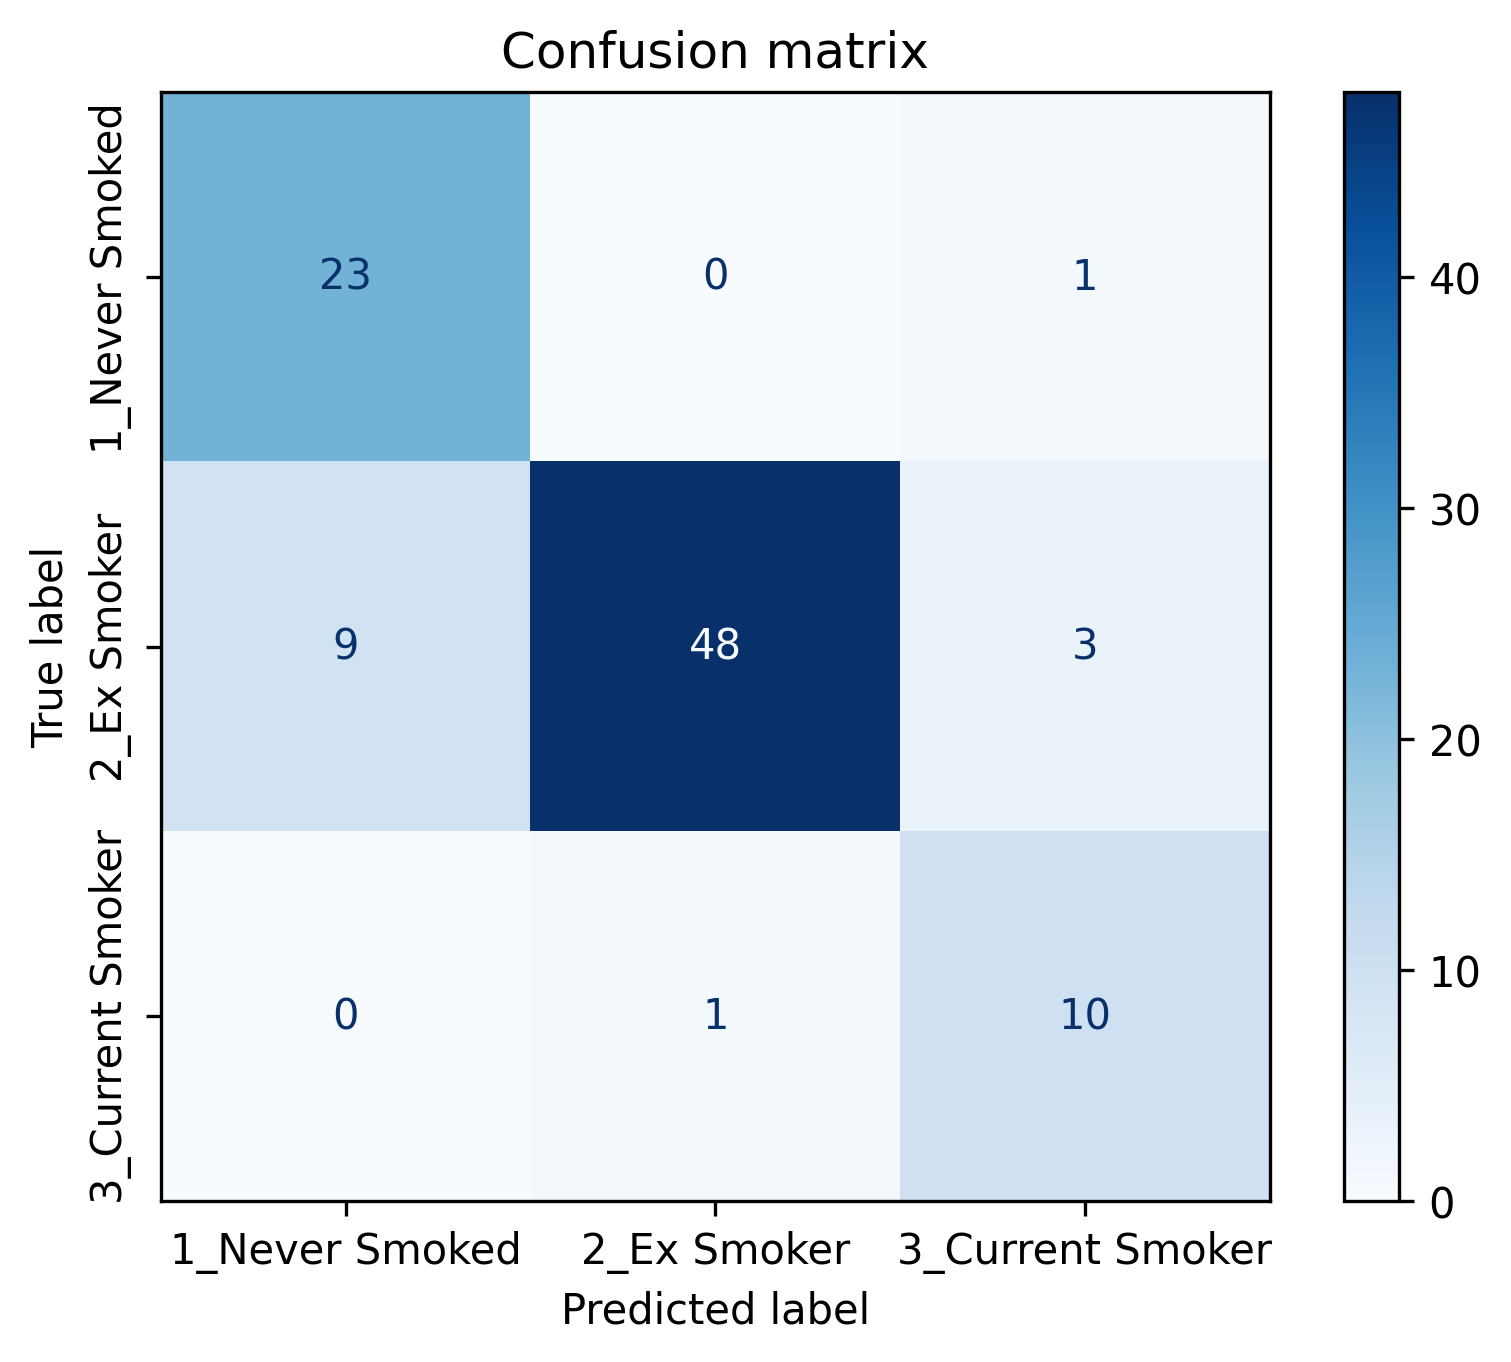
\includegraphics[width=\linewidth]{cohort1/test_confusion_matrix.png}
        \caption{Counts}
    \end{subfigure}
    \hfill
    \begin{subfigure}{0.49\linewidth}
        \centering
        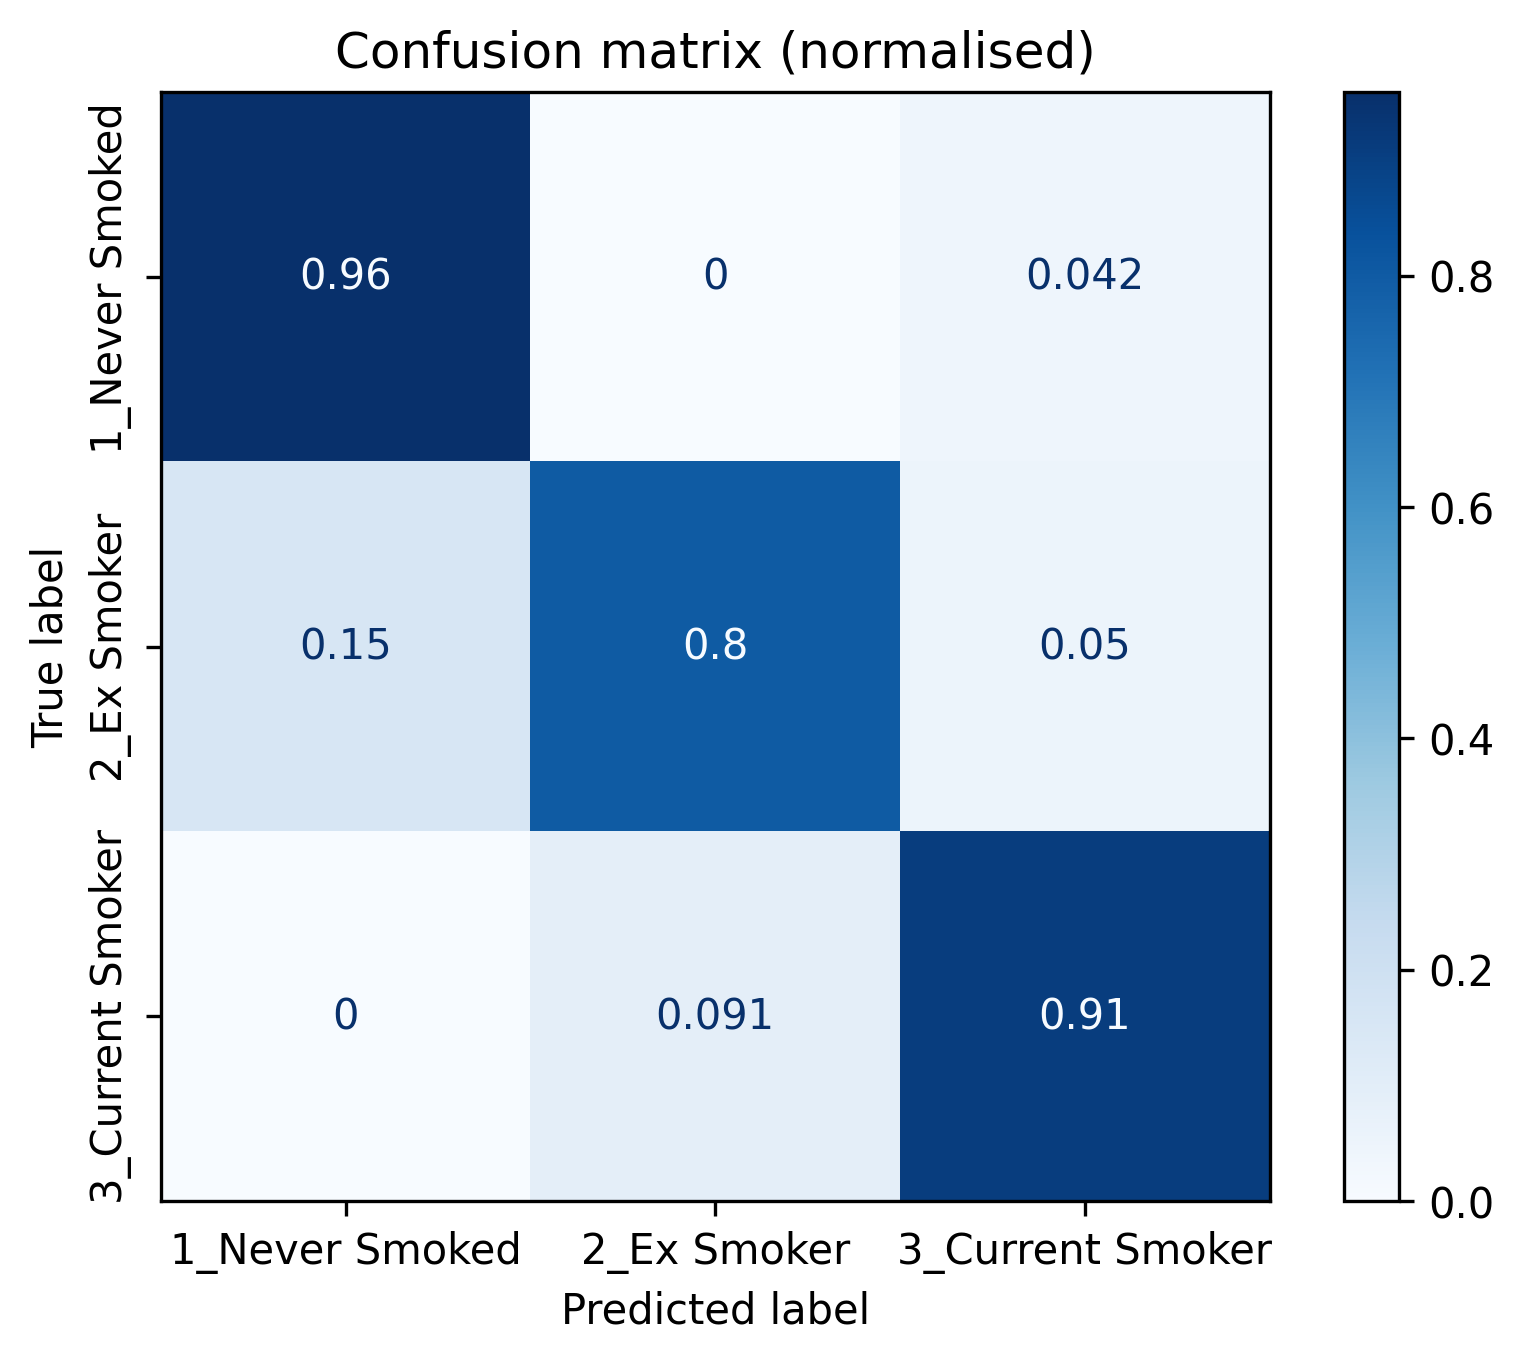
\includegraphics[width=\linewidth]{cohort1/test_confusion_matrix_normalised.png}
        \caption{Percentages}
    \end{subfigure}
    \caption[Confusion matrices (Cohort 1 - Test)]{Confusion matrices (Cohort 1 - Test). The first confusion matrix displays classification and misclassification counts, while the second confusion matrix normalises these into percentages. The model correctly classified each class with high accuracy in this cohort.}
    \label{fig:cohort1-confusion-matrix}
\end{figure}

\begin{figure}[p]
    \centering
    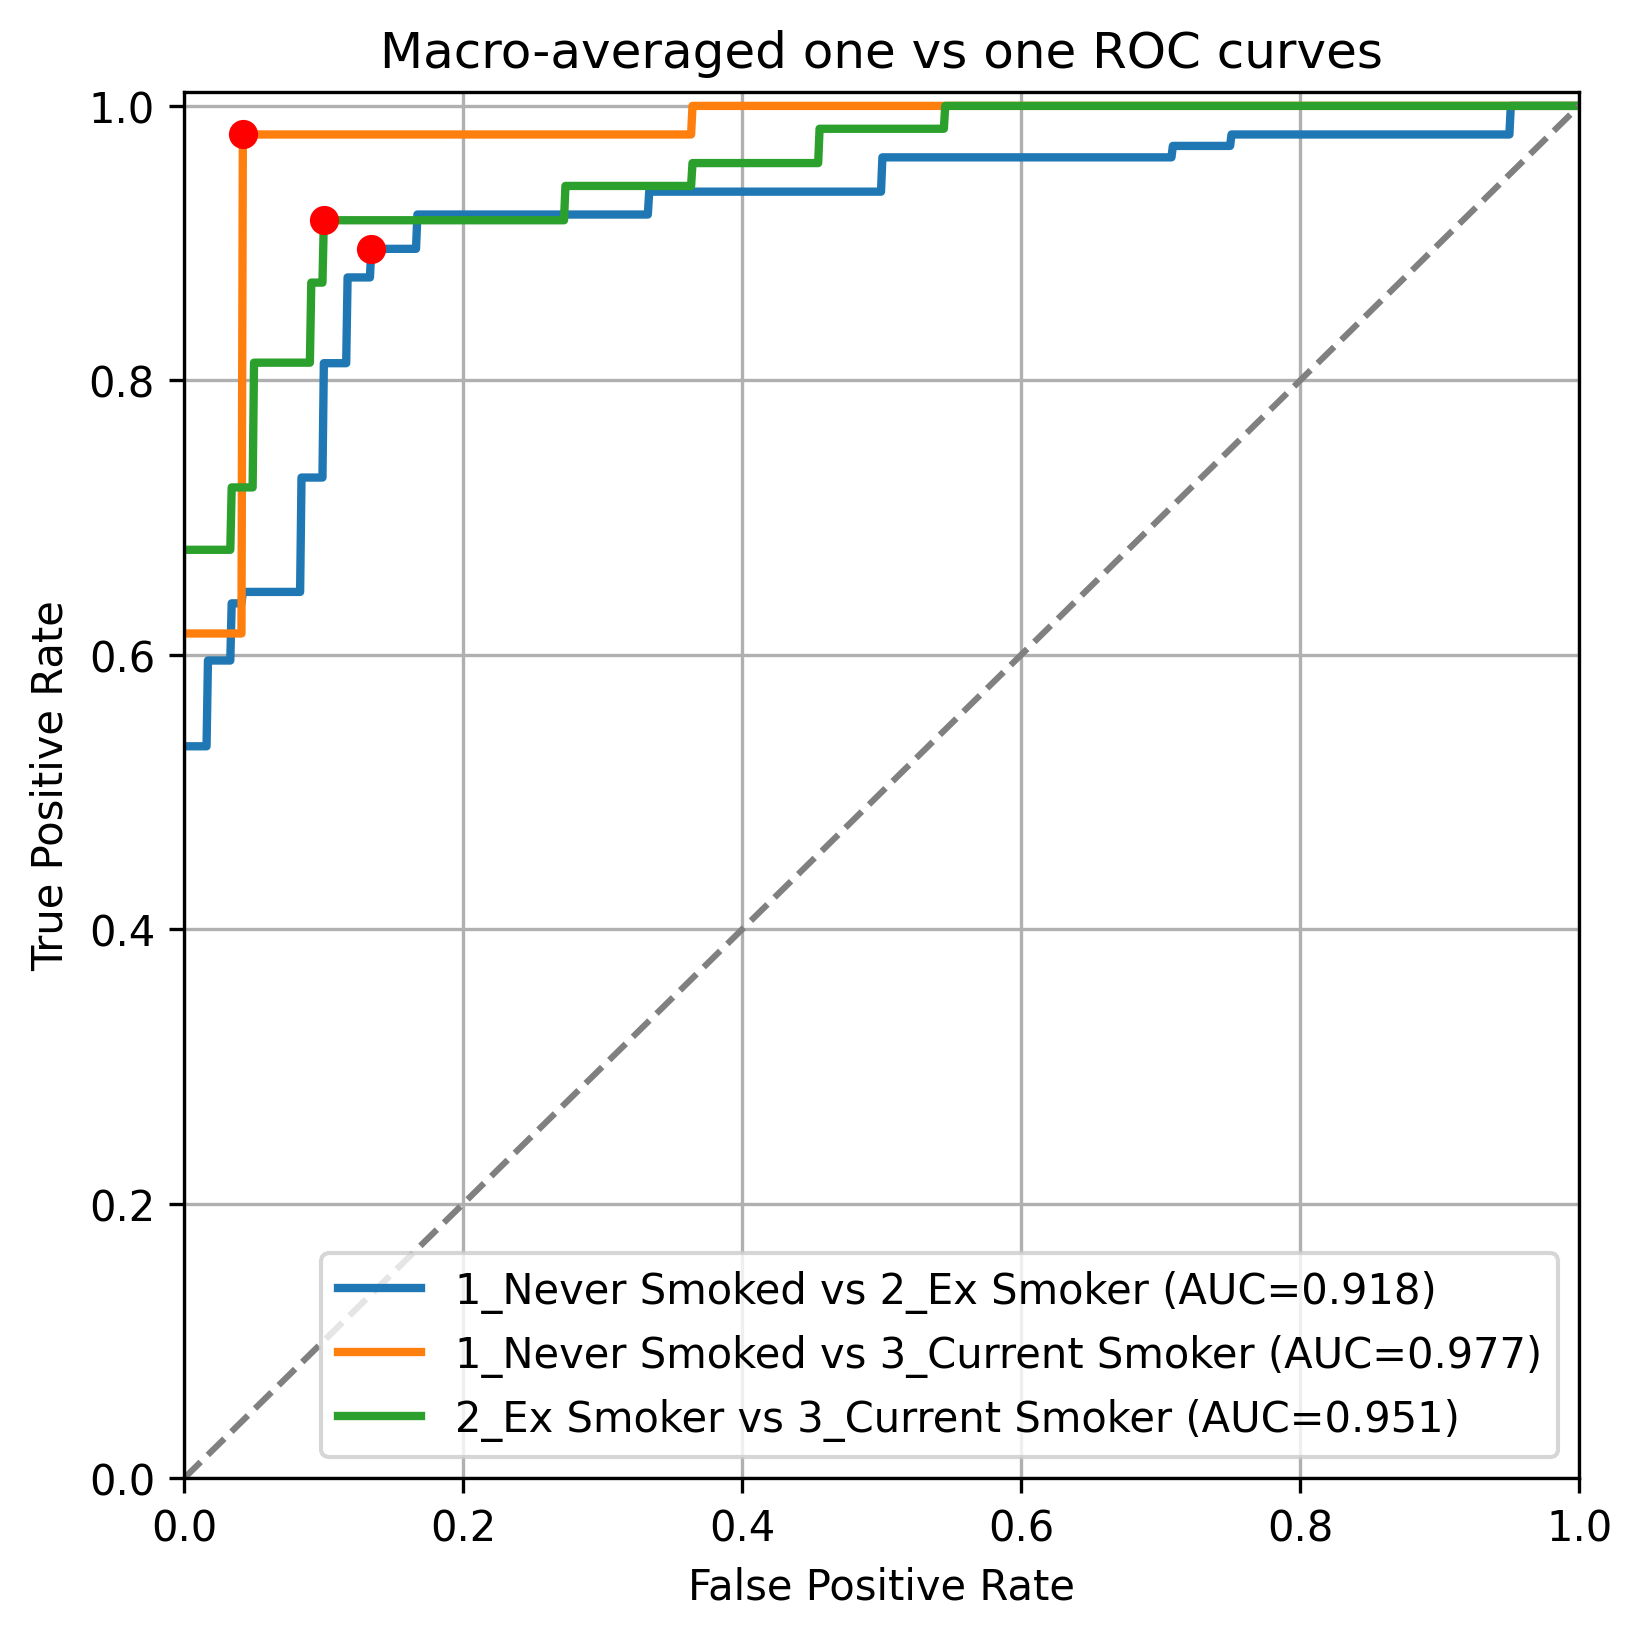
\includegraphics[width=0.7\linewidth]{cohort1/test_macro_ovo_roc.png}
    \caption[Macro-averaged ROC curves (Cohort 1 - Test)]{Macro-averaged ROC curves (Cohort 1 - Test). Each curve aggregates the two relevant class-specific predictors into a single ROC curve, giving a single curve which evaluates the entire model's performance separating two classes. The model's separation of all three classes was excellent in this cohort.}
    \label{fig:cohort1-macro-rocs}
\end{figure}

\begin{figure}[p]
    \centering
    \begin{subfigure}{0.46\linewidth}
        \centering
        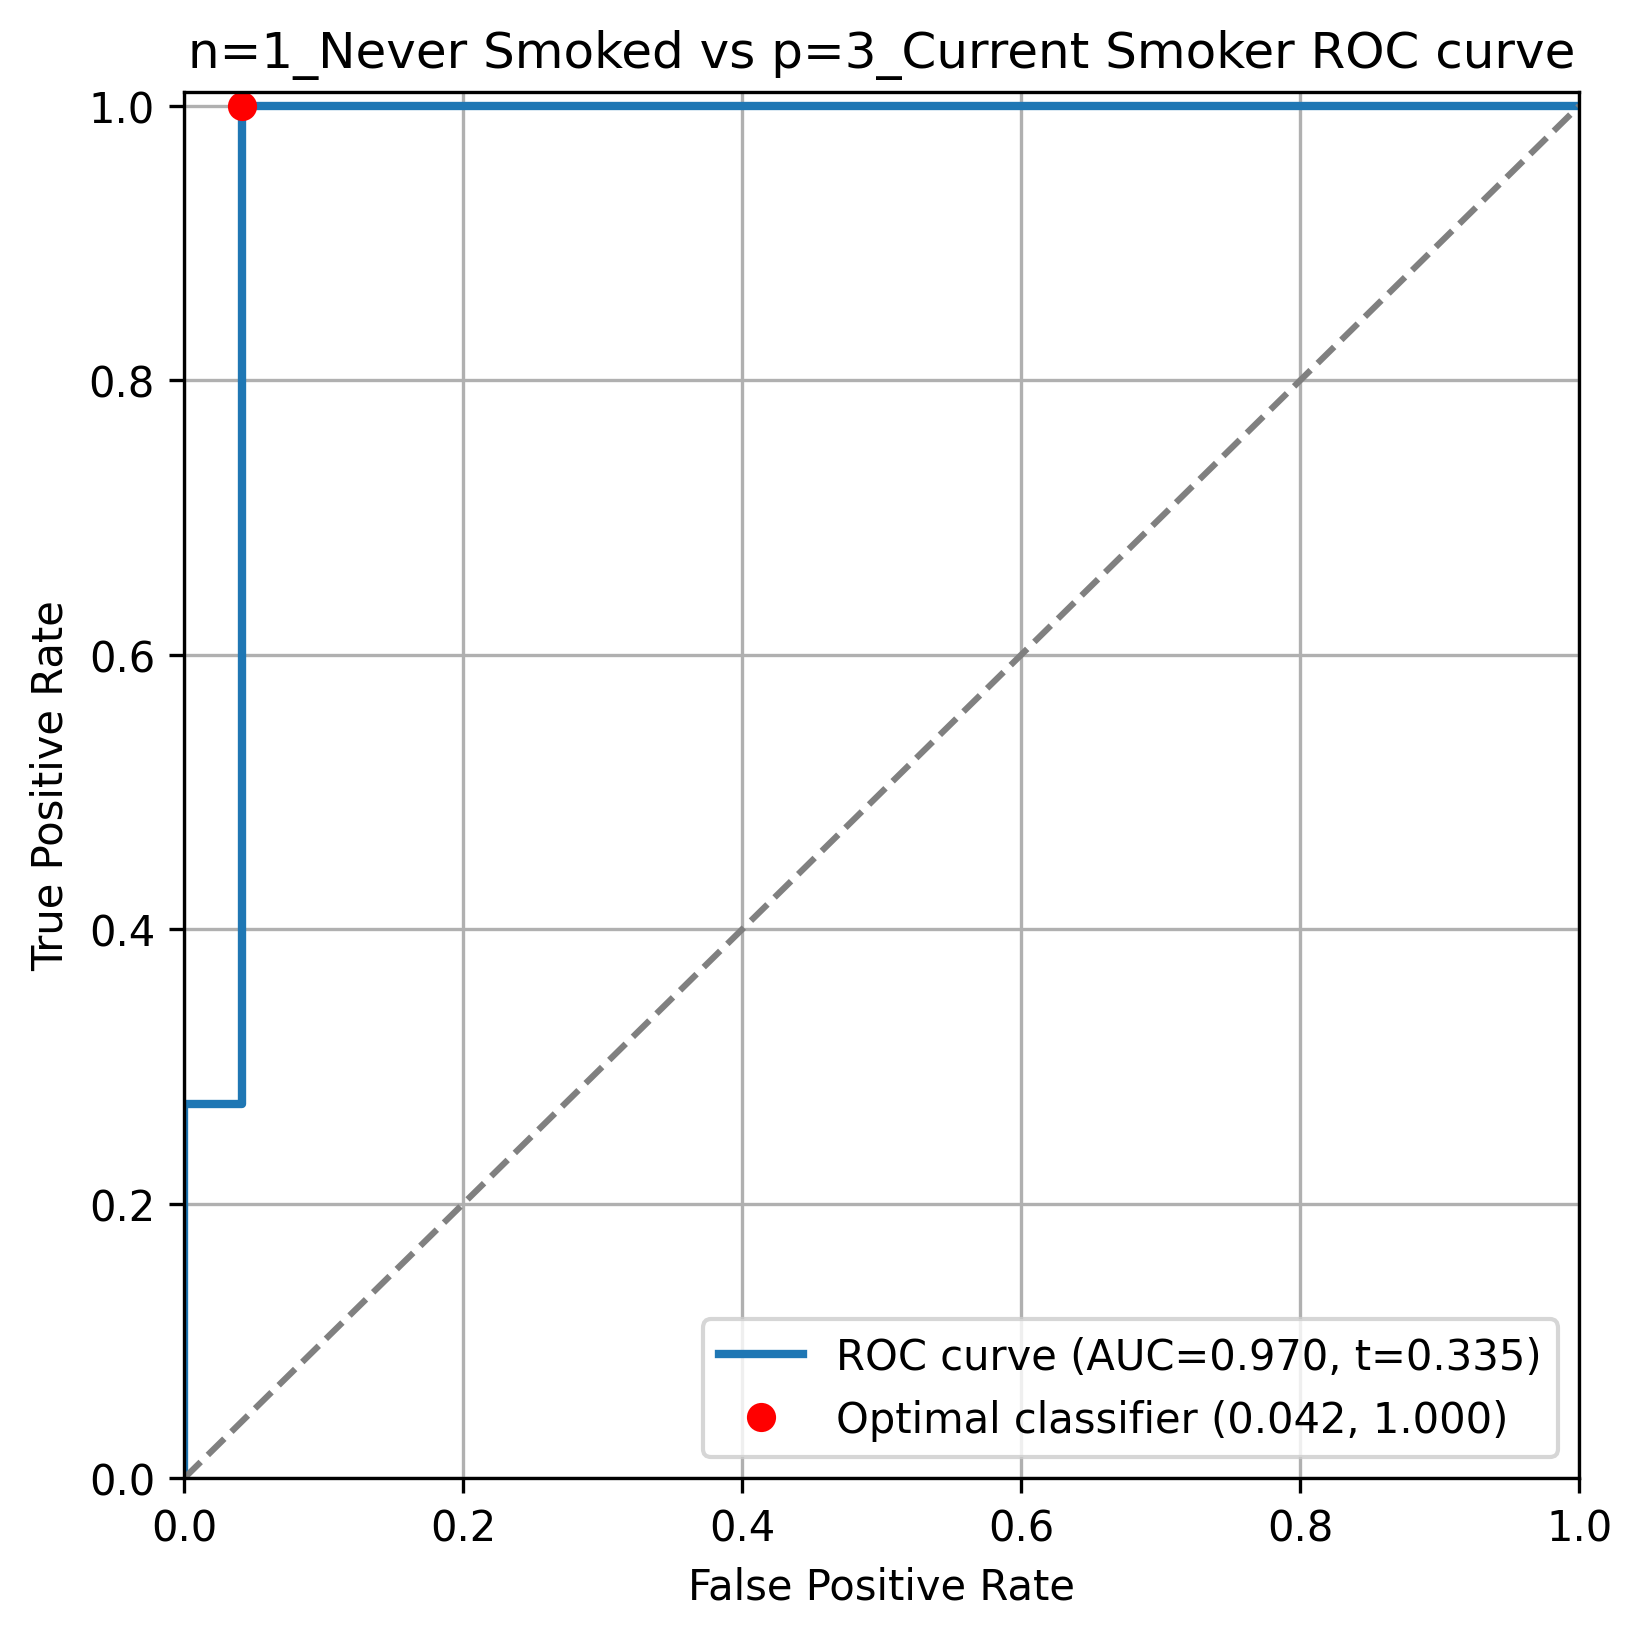
\includegraphics[width=\linewidth]{cohort1/test_1v3_roc.png}
    \end{subfigure}
    \hspace{4mm}
    \begin{subfigure}{0.46\linewidth}
        \centering
        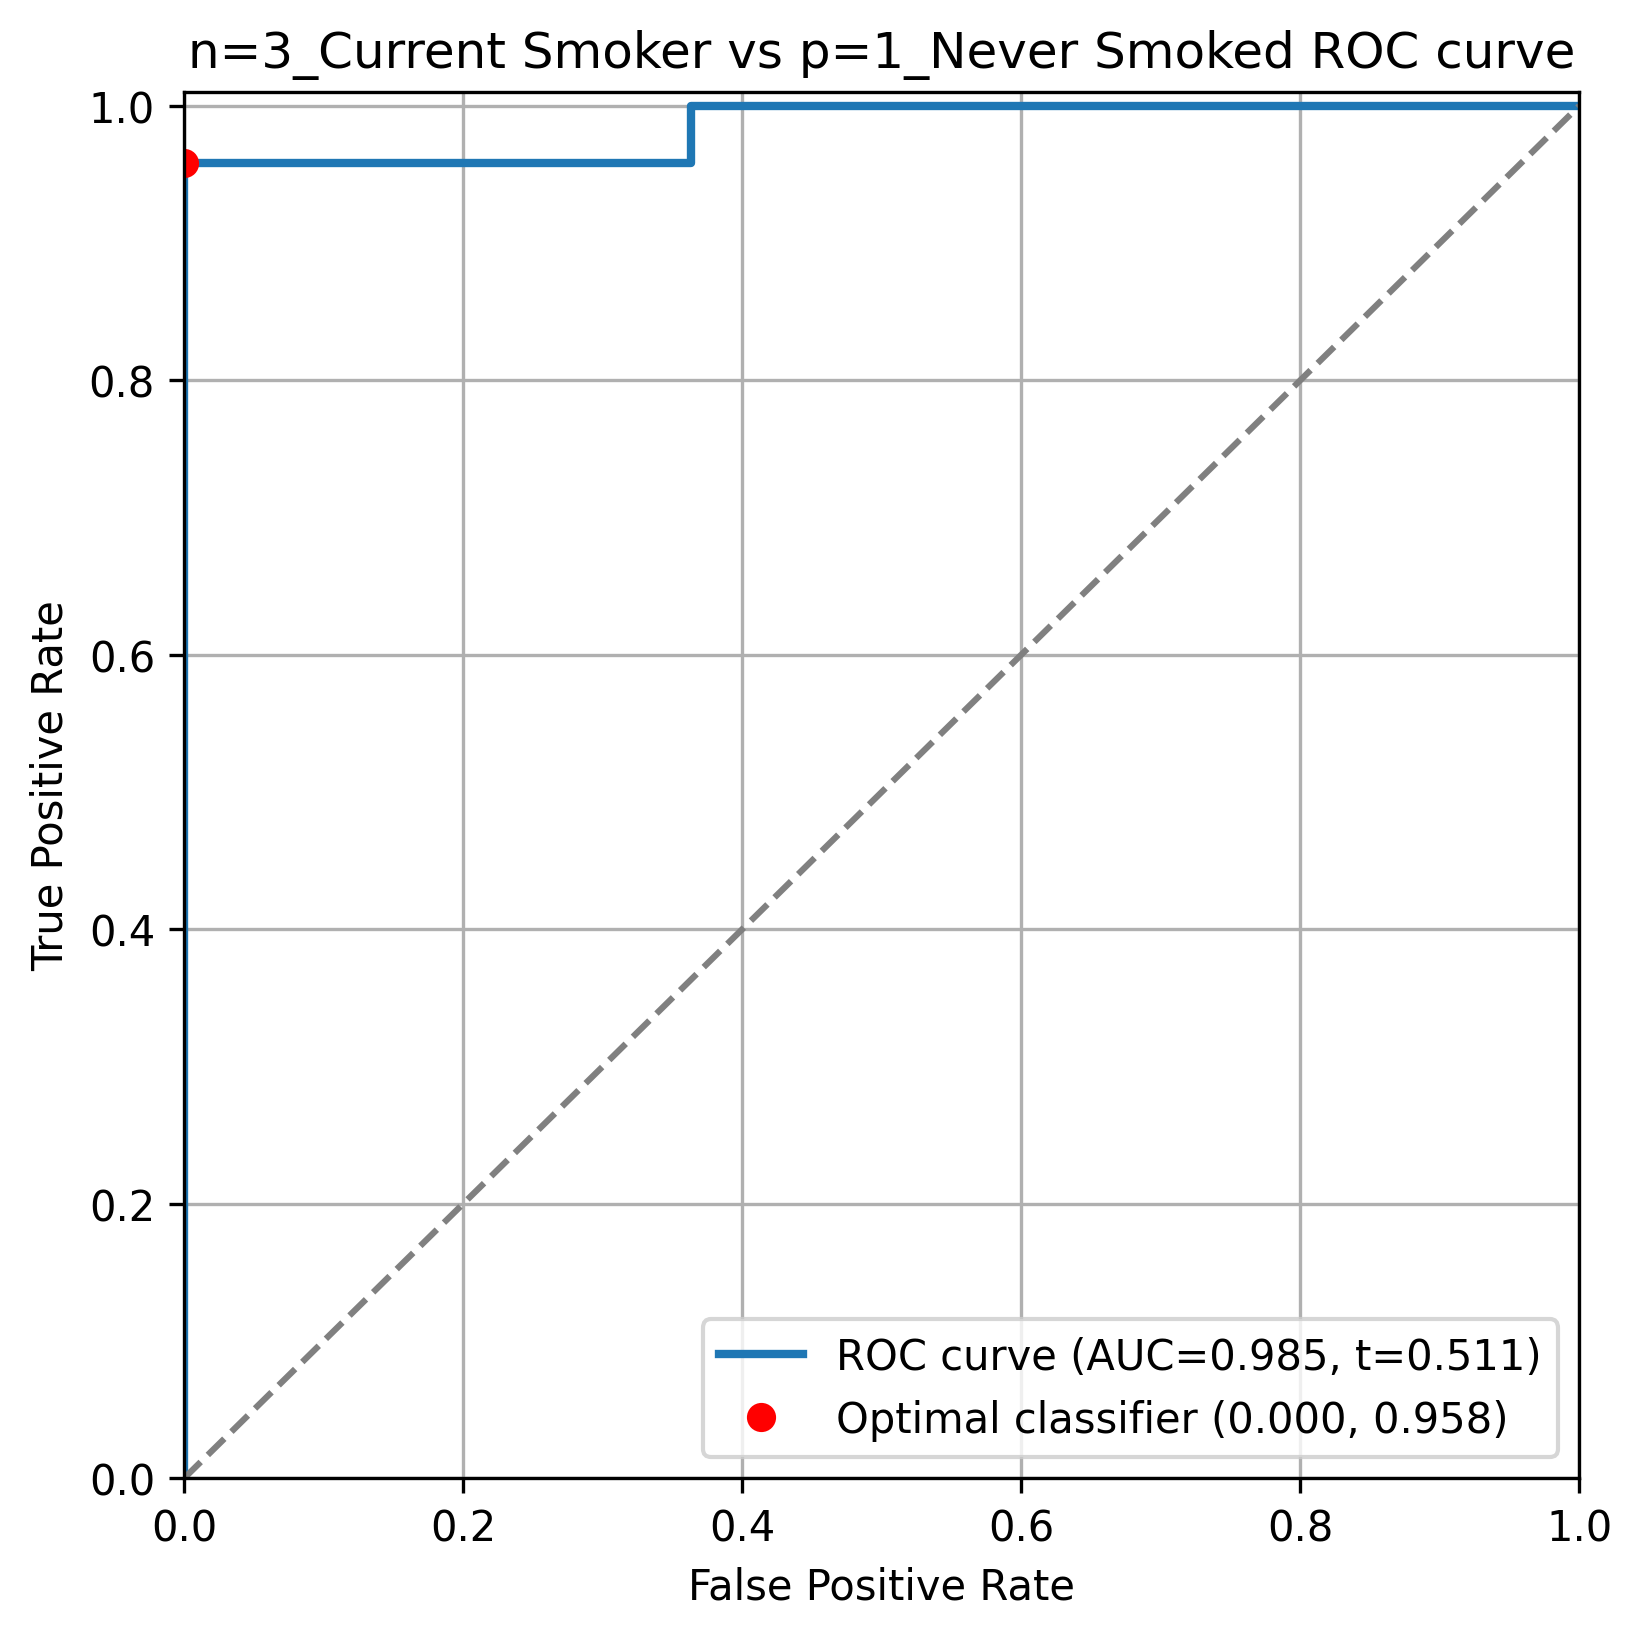
\includegraphics[width=\linewidth]{cohort1/test_3v1_roc.png}
    \end{subfigure}

    \begin{subfigure}{0.46\linewidth}
        \centering
        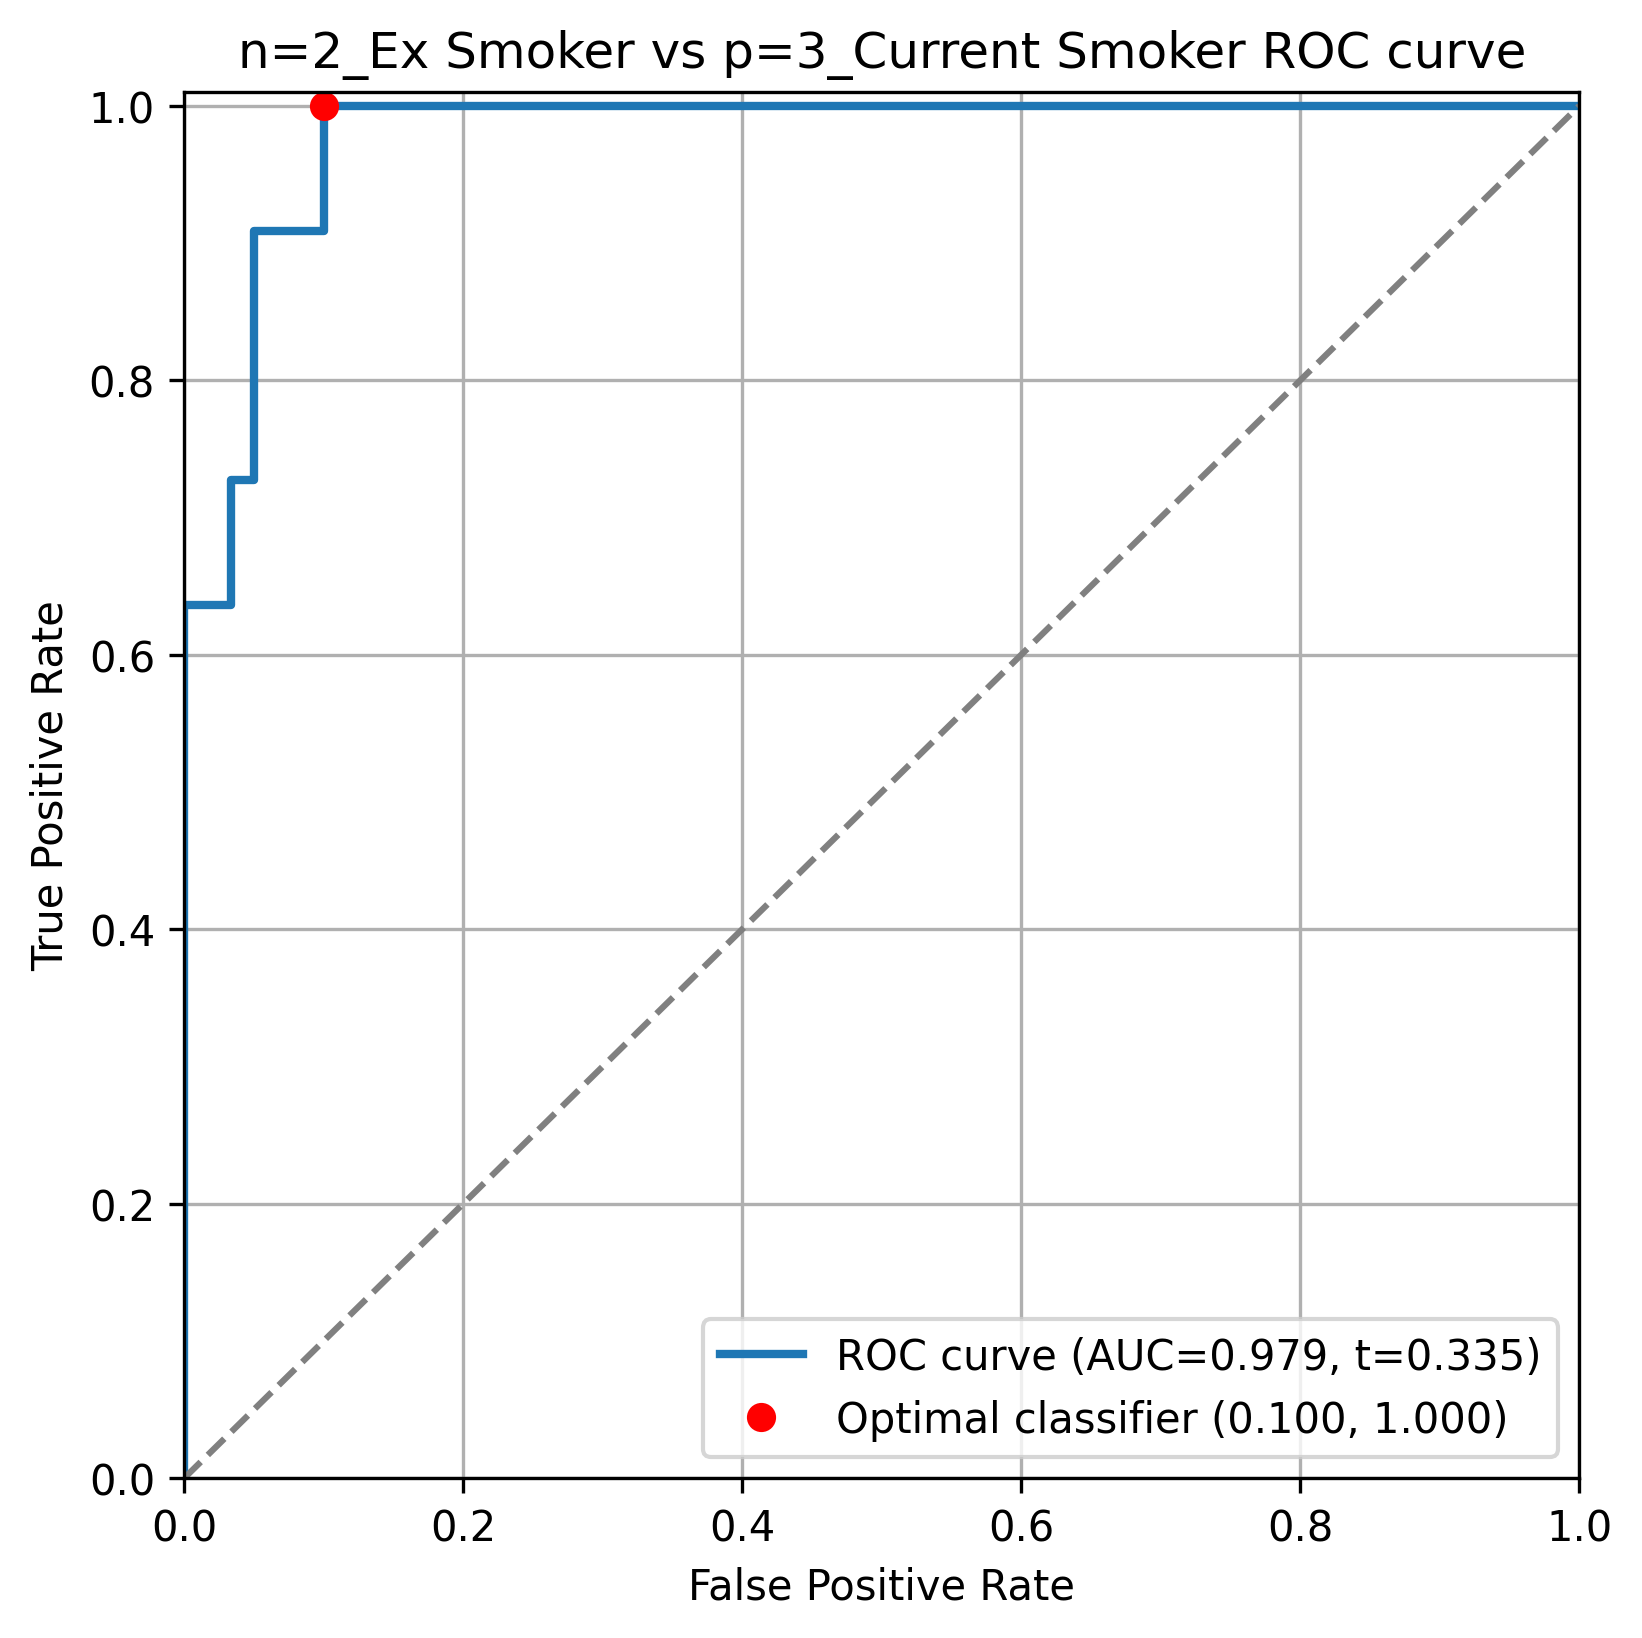
\includegraphics[width=\linewidth]{cohort1/test_2v3_roc.png}
    \end{subfigure}
    \hspace{4mm}
    \begin{subfigure}{0.46\linewidth}
        \centering
        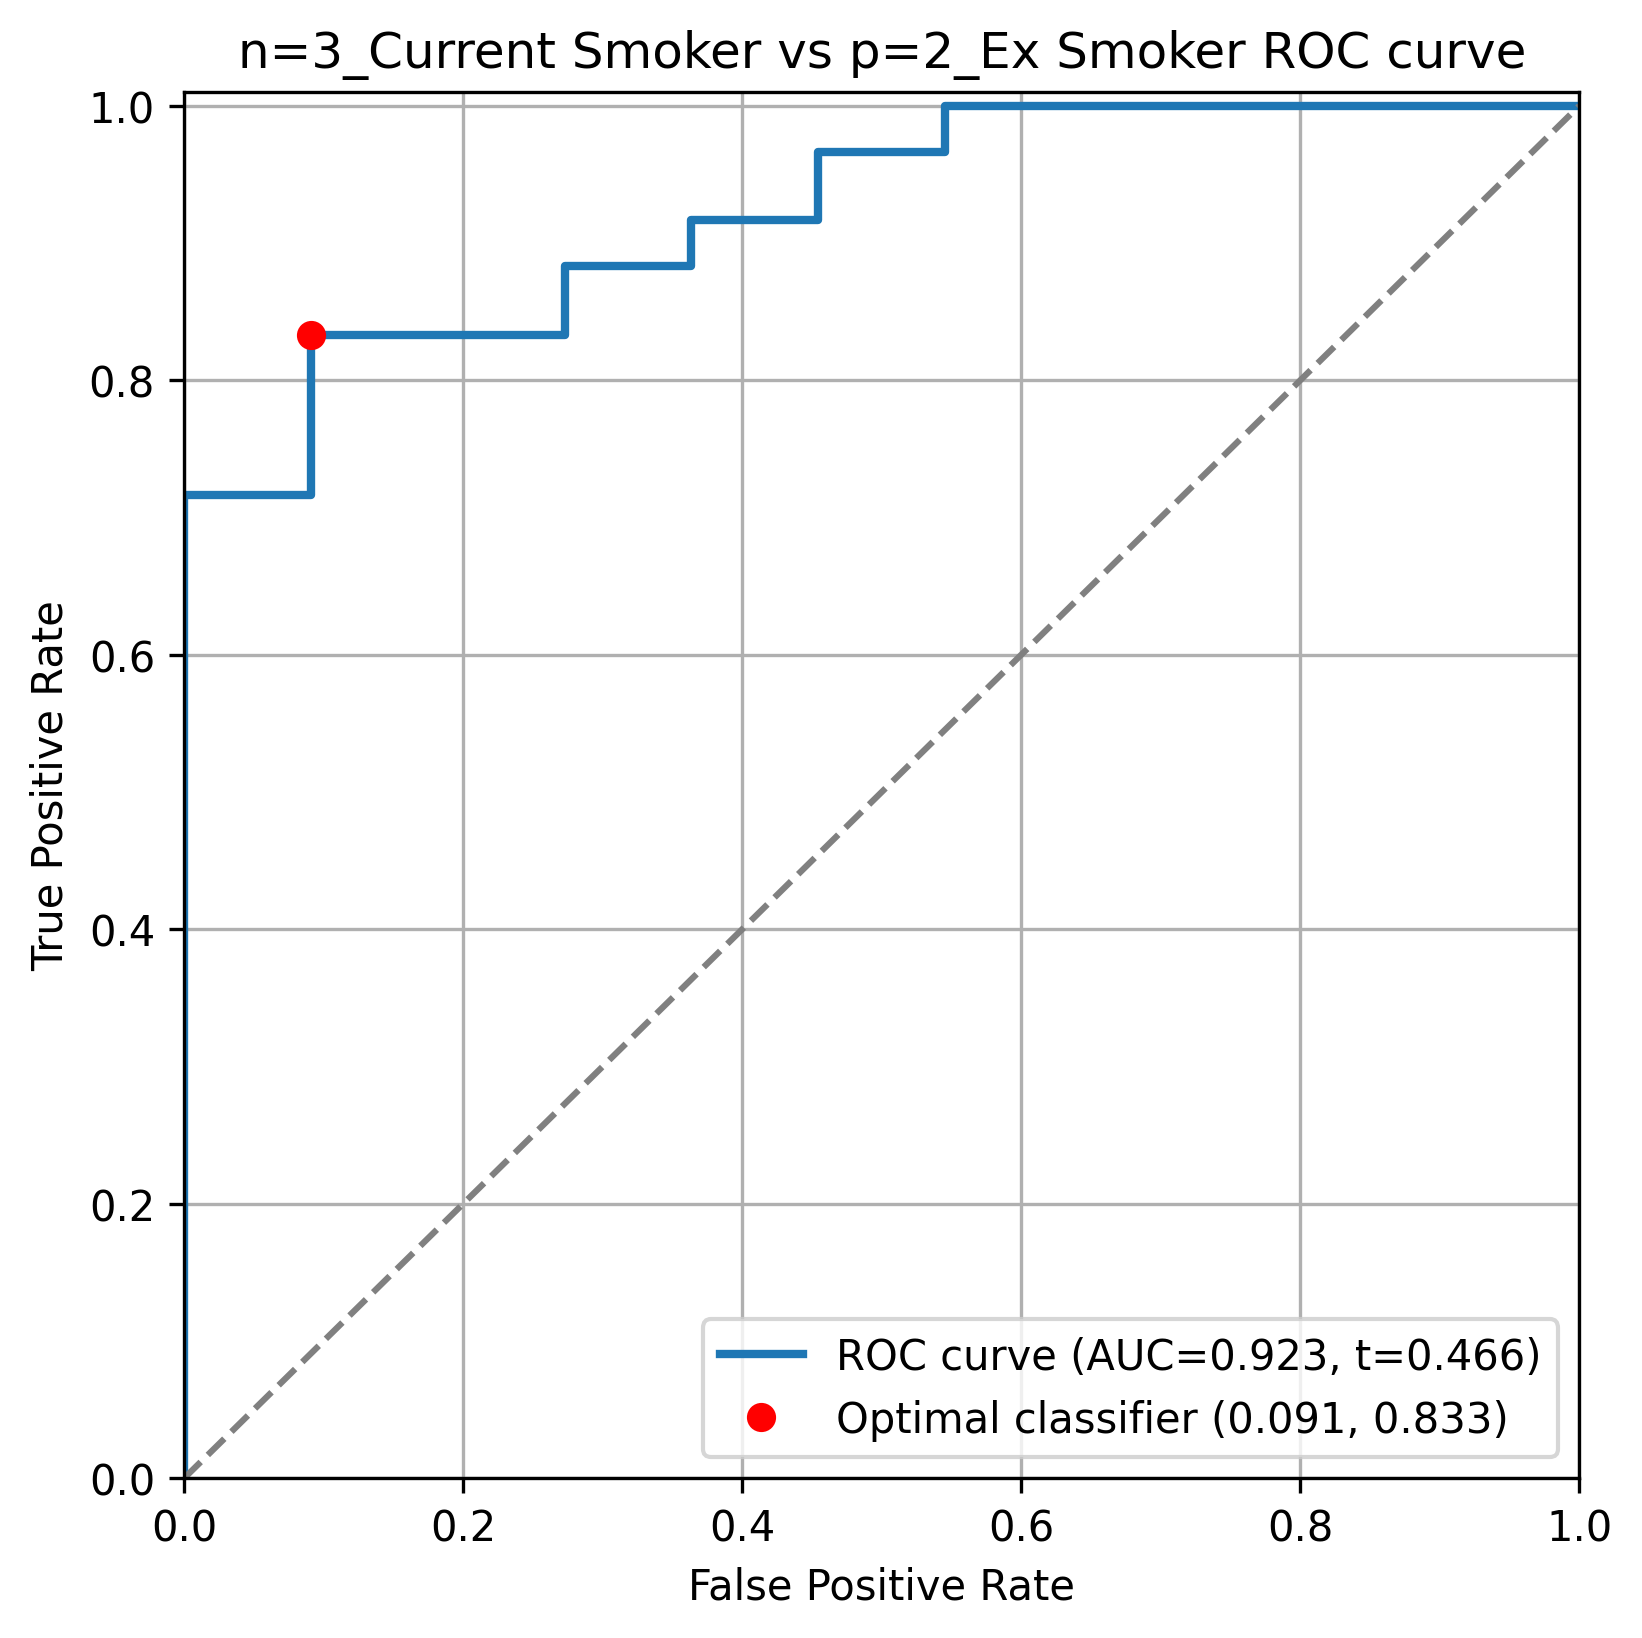
\includegraphics[width=\linewidth]{cohort1/test_3v2_roc.png}
    \end{subfigure}

    \begin{subfigure}{0.46\linewidth}
        \centering
        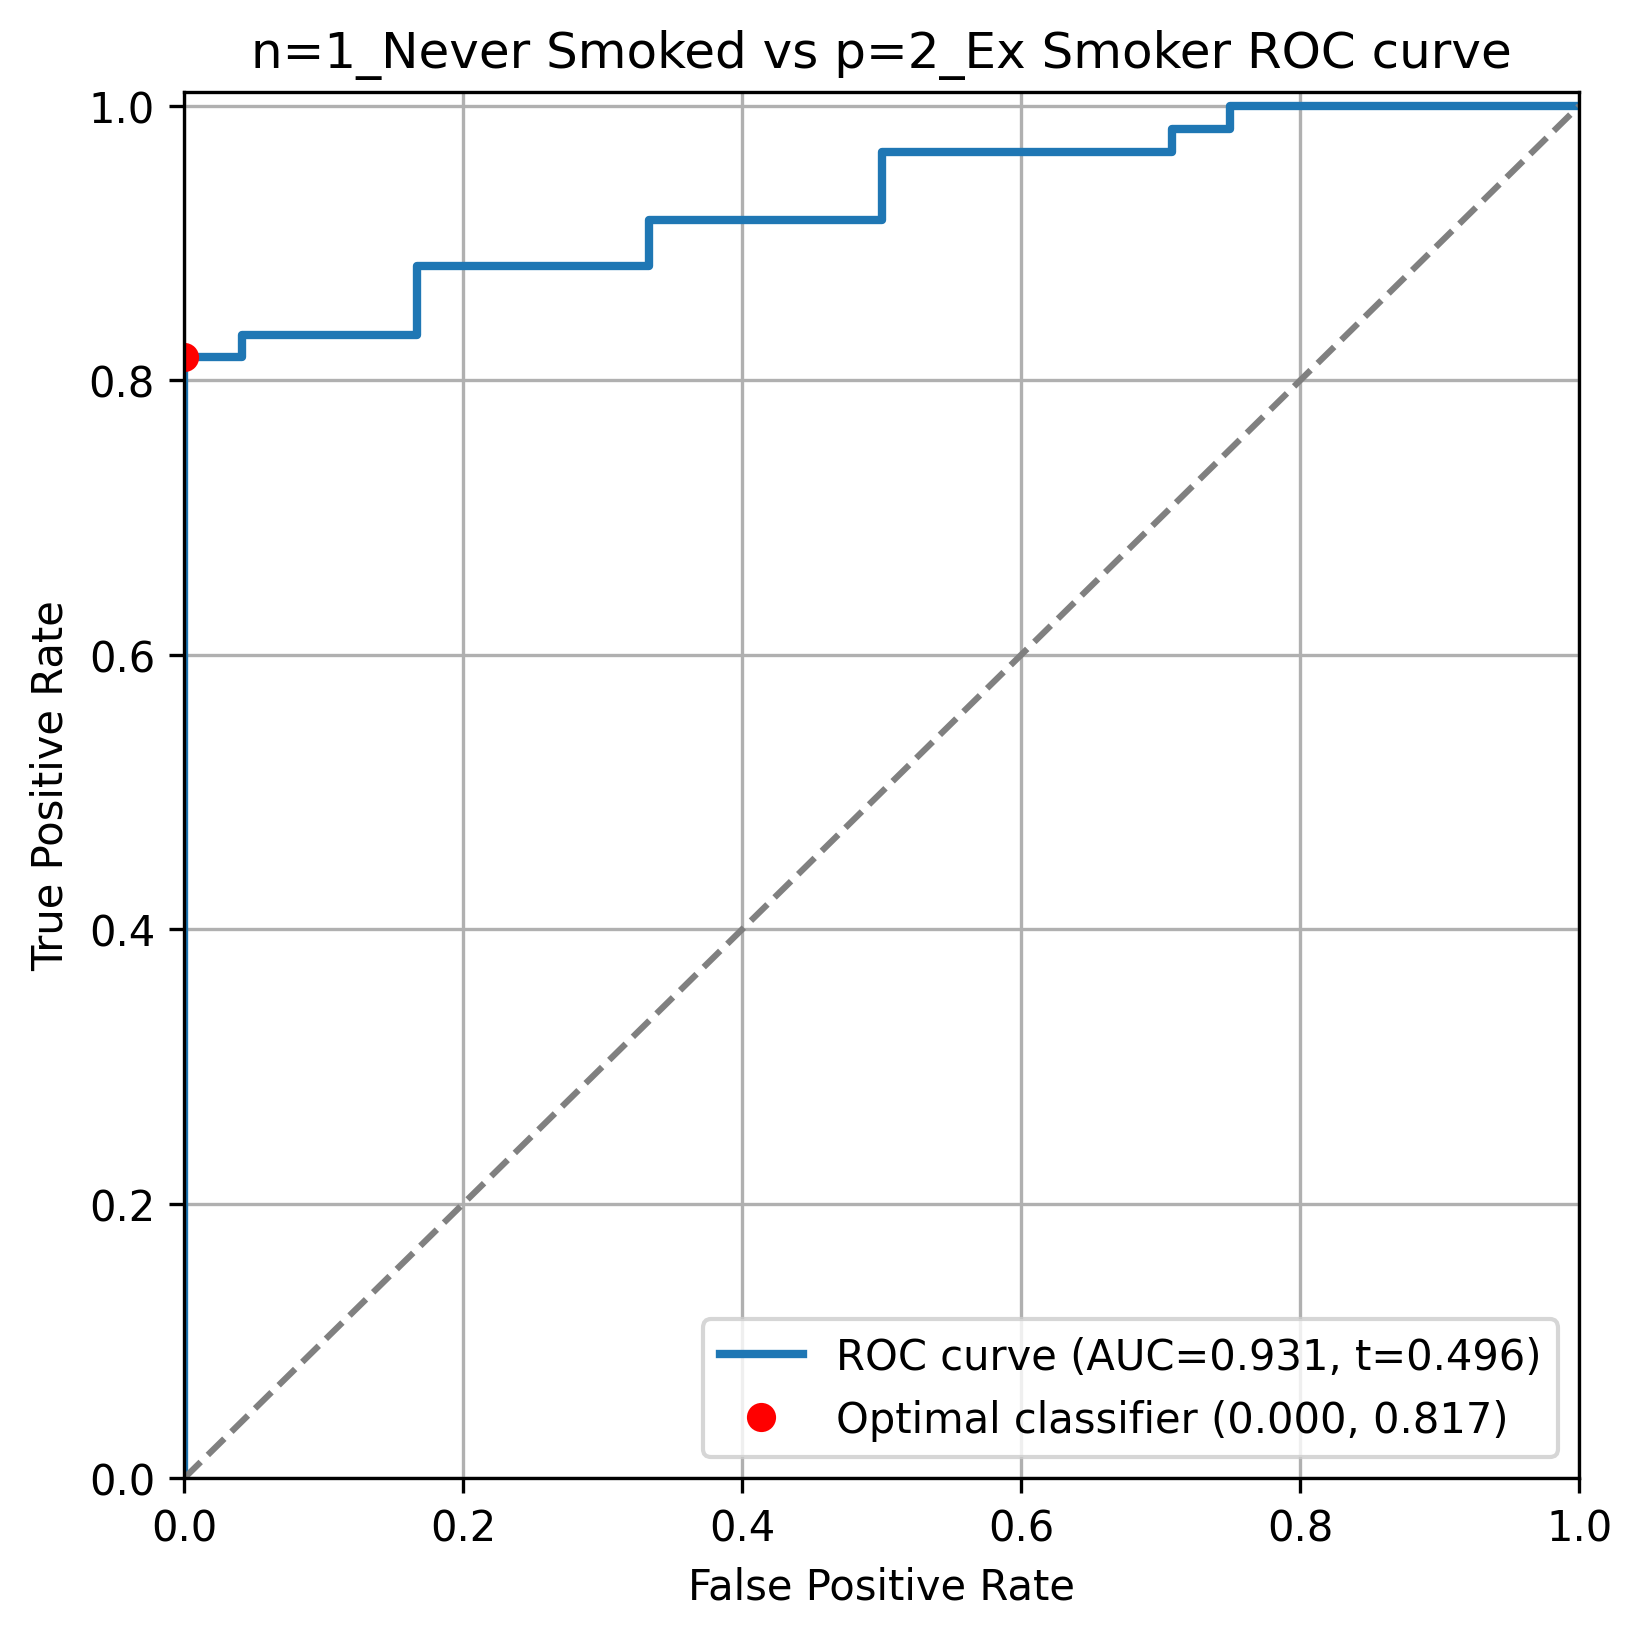
\includegraphics[width=\linewidth]{cohort1/test_1v2_roc.png}
    \end{subfigure}
    \hspace{4mm}
    \begin{subfigure}{0.46\linewidth}
        \centering
        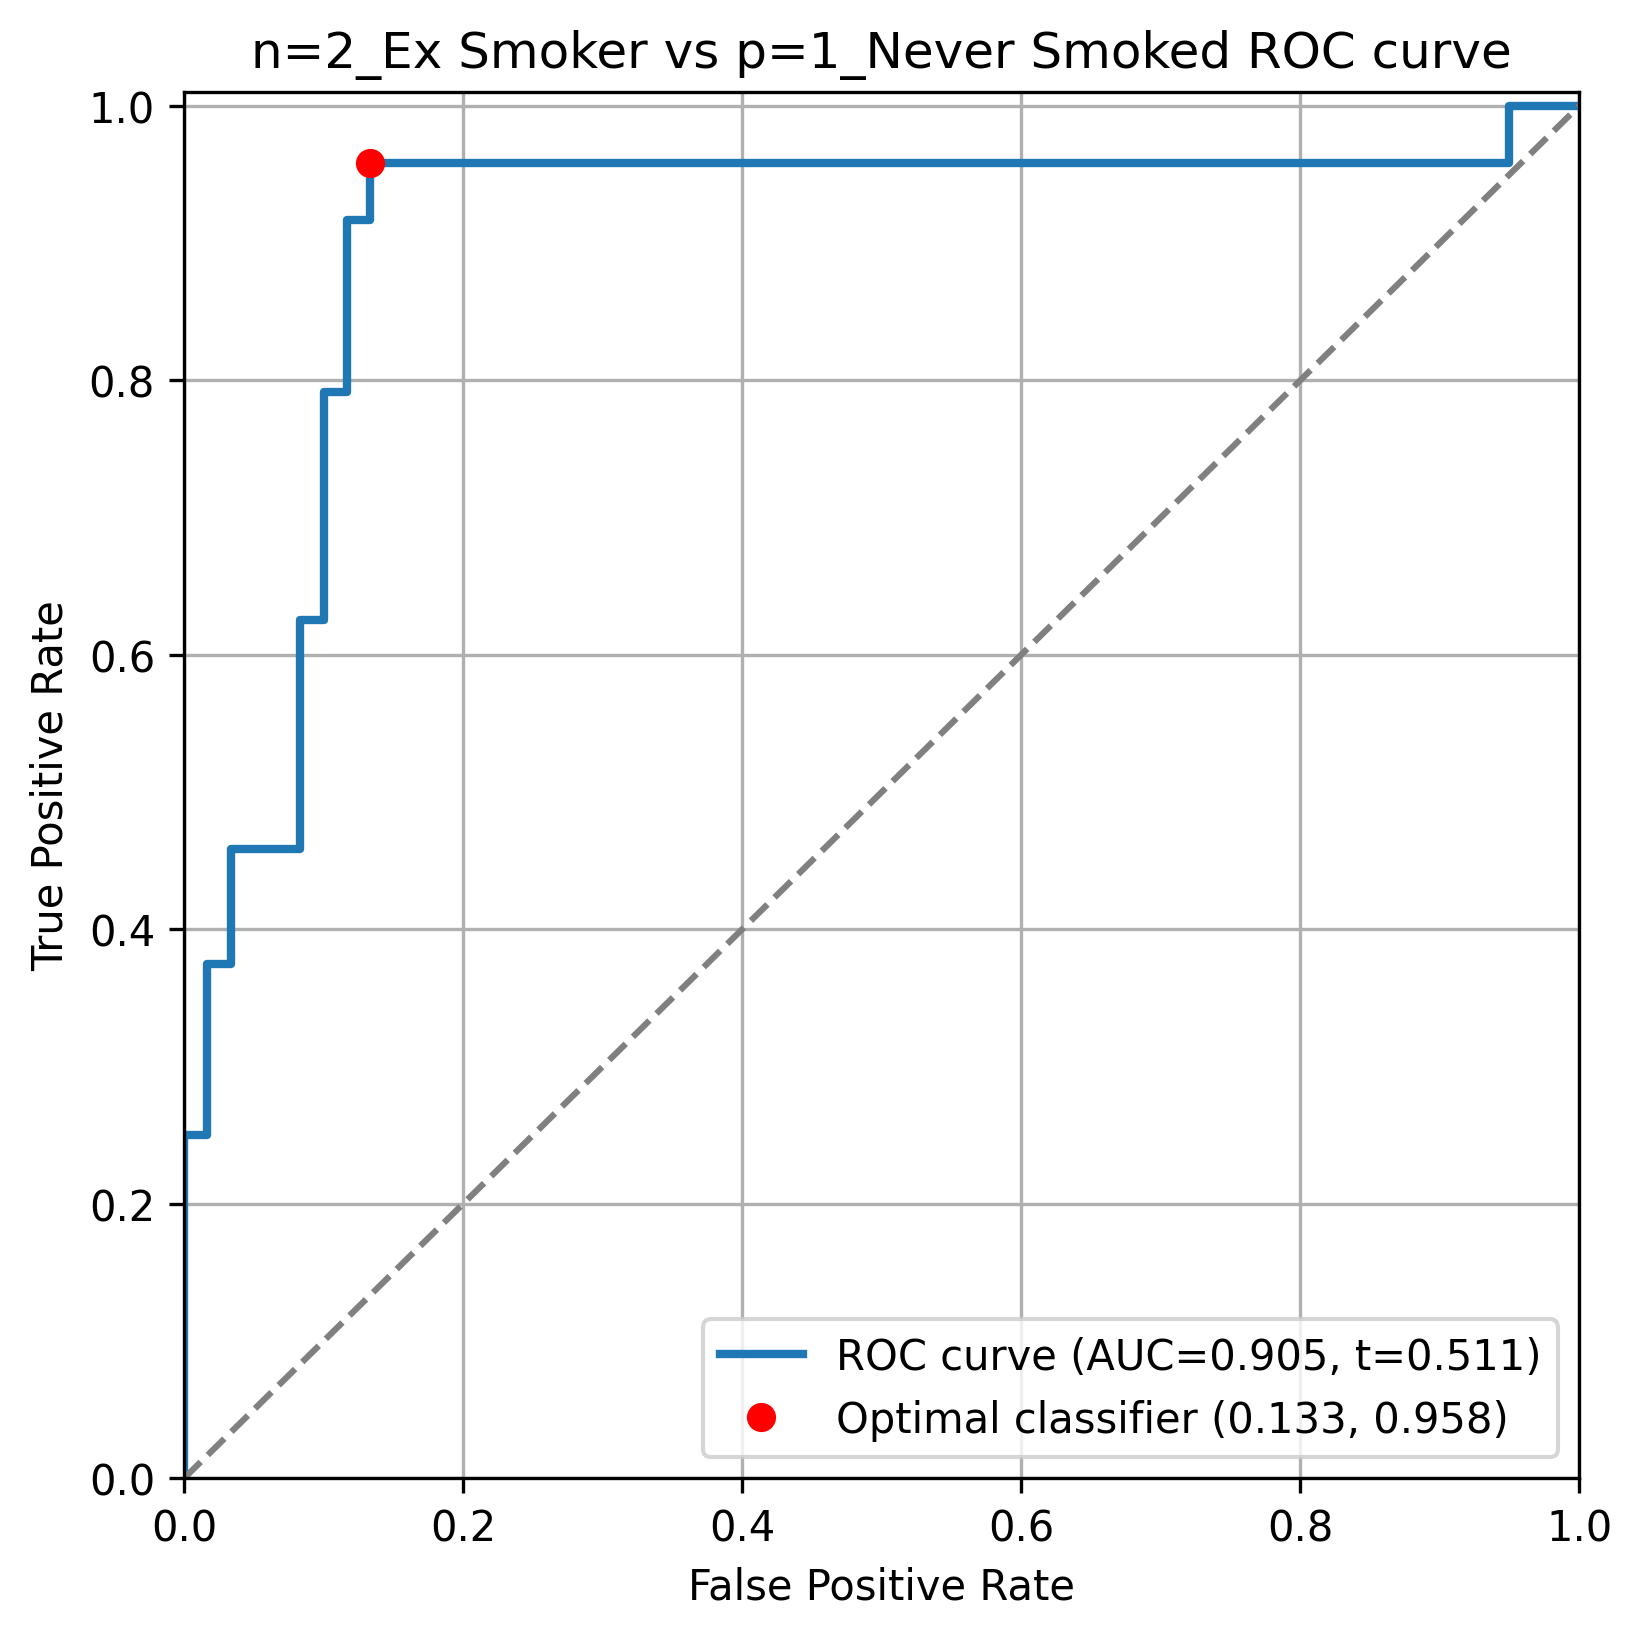
\includegraphics[width=\linewidth]{cohort1/test_2v1_roc.png}
    \end{subfigure}
    \caption[Class-specific predictor ROC curves (Cohort 1 - Test)]{OvO class-specific predictor ROC curves (Cohort 1). Each curve shows a single class-specific predictor's ability to separate two classes, using the probability outputs for the given predictor. The predictor used for each curve corresponds to the positive class. Each class-specific predictor achieved excellent performance separating each pair of classes in this cohort.}
    \label{fig:cohort1-initial-rocs}
\end{figure}

ENSS achieved excellent predictive performance on the Cohort 1 hold-out test set. The classification performance on this dataset can be seen in Figure \ref{fig:cohort1-confusion-matrix}. Out of the 95 individuals in this dataset, only 15 were misclassified by the model. Per class, \SI{92}{\percent} of never-smokers were correctly classified, while \SI{82}{\percent} of both ex-smokers and current-smokers were correctly classified.

The model's ability to separate classes was also evaluated. Macro-averaged OvO ROC curves for the entire model can be seen in Figure \ref{fig:cohort1-macro-rocs}. These were generated by aggregating OvO ROC curves of the class-specific predictors, seen in Figure \ref{fig:cohort1-initial-rocs}. The model achieved macro-averaged OvO ROC-AUCs of: 0.977 for separating never-smokers from current-smokers, 0.941 for separating ex-smokers from current-smokers, and 0.909 for separating never-smokers from ex-smokers. Overall, we can see the model achieved excellent performance separating each of the pairs of classes.

\begin{figure}[p]
    \centering
    \begin{subfigure}{0.48\linewidth}
        \centering
        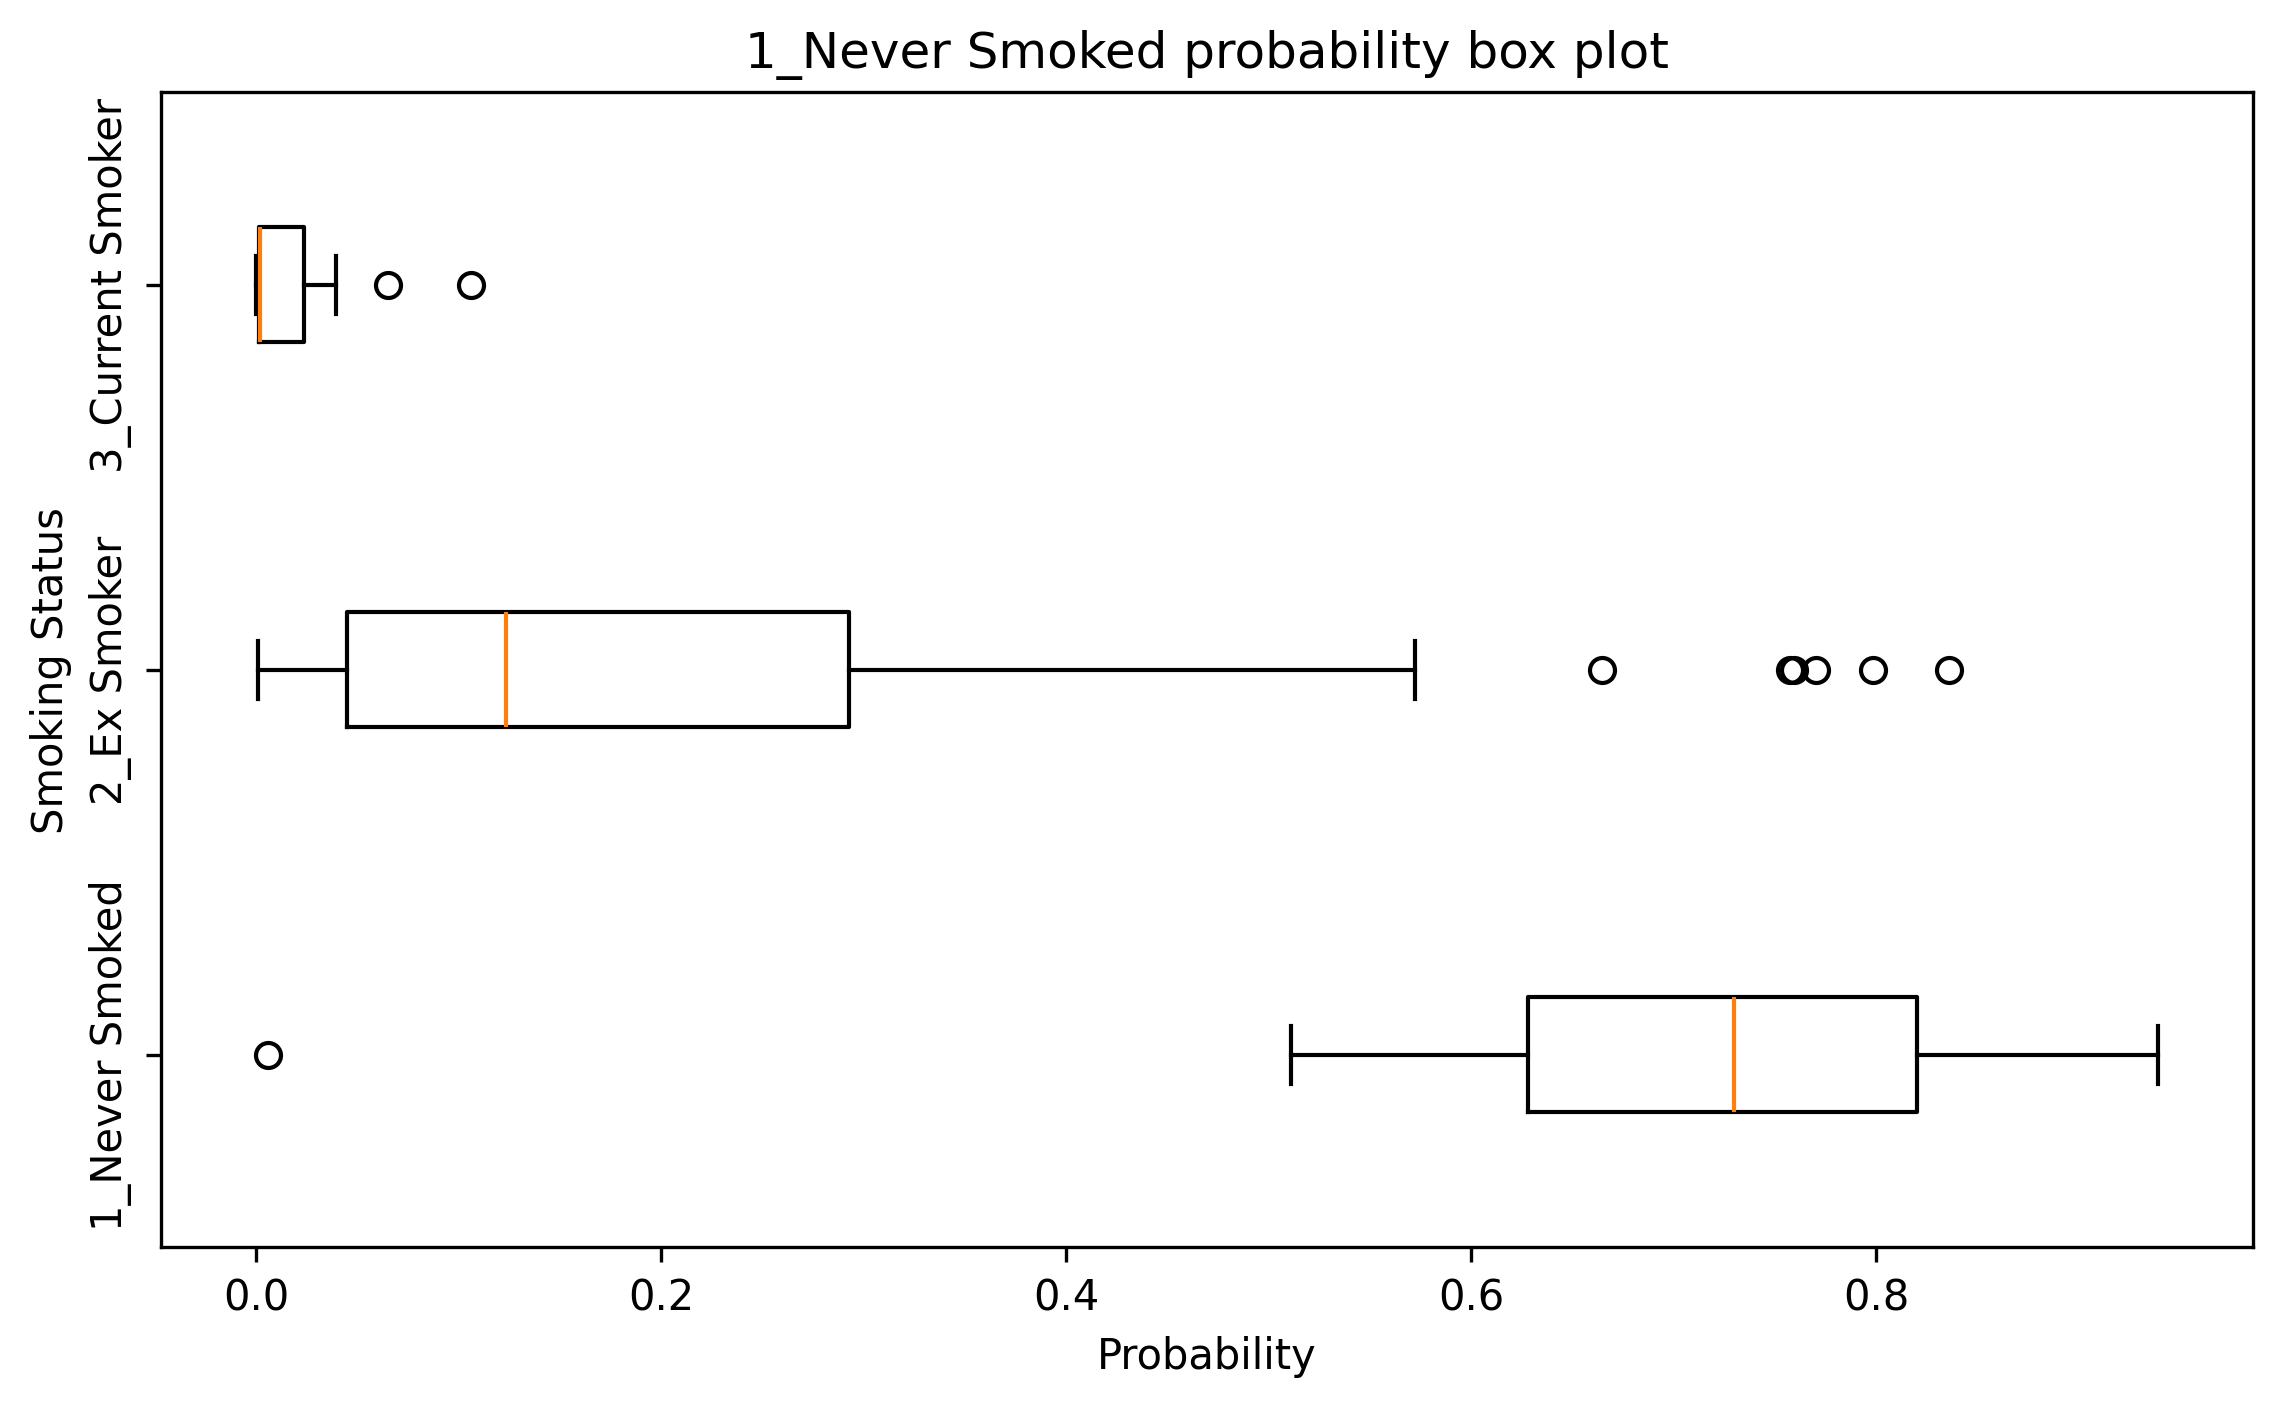
\includegraphics[width=\linewidth]{cohort1/test_boxplot_1.png}
    \end{subfigure}
    \hfill
    \begin{subfigure}{0.48\linewidth}
        \centering
        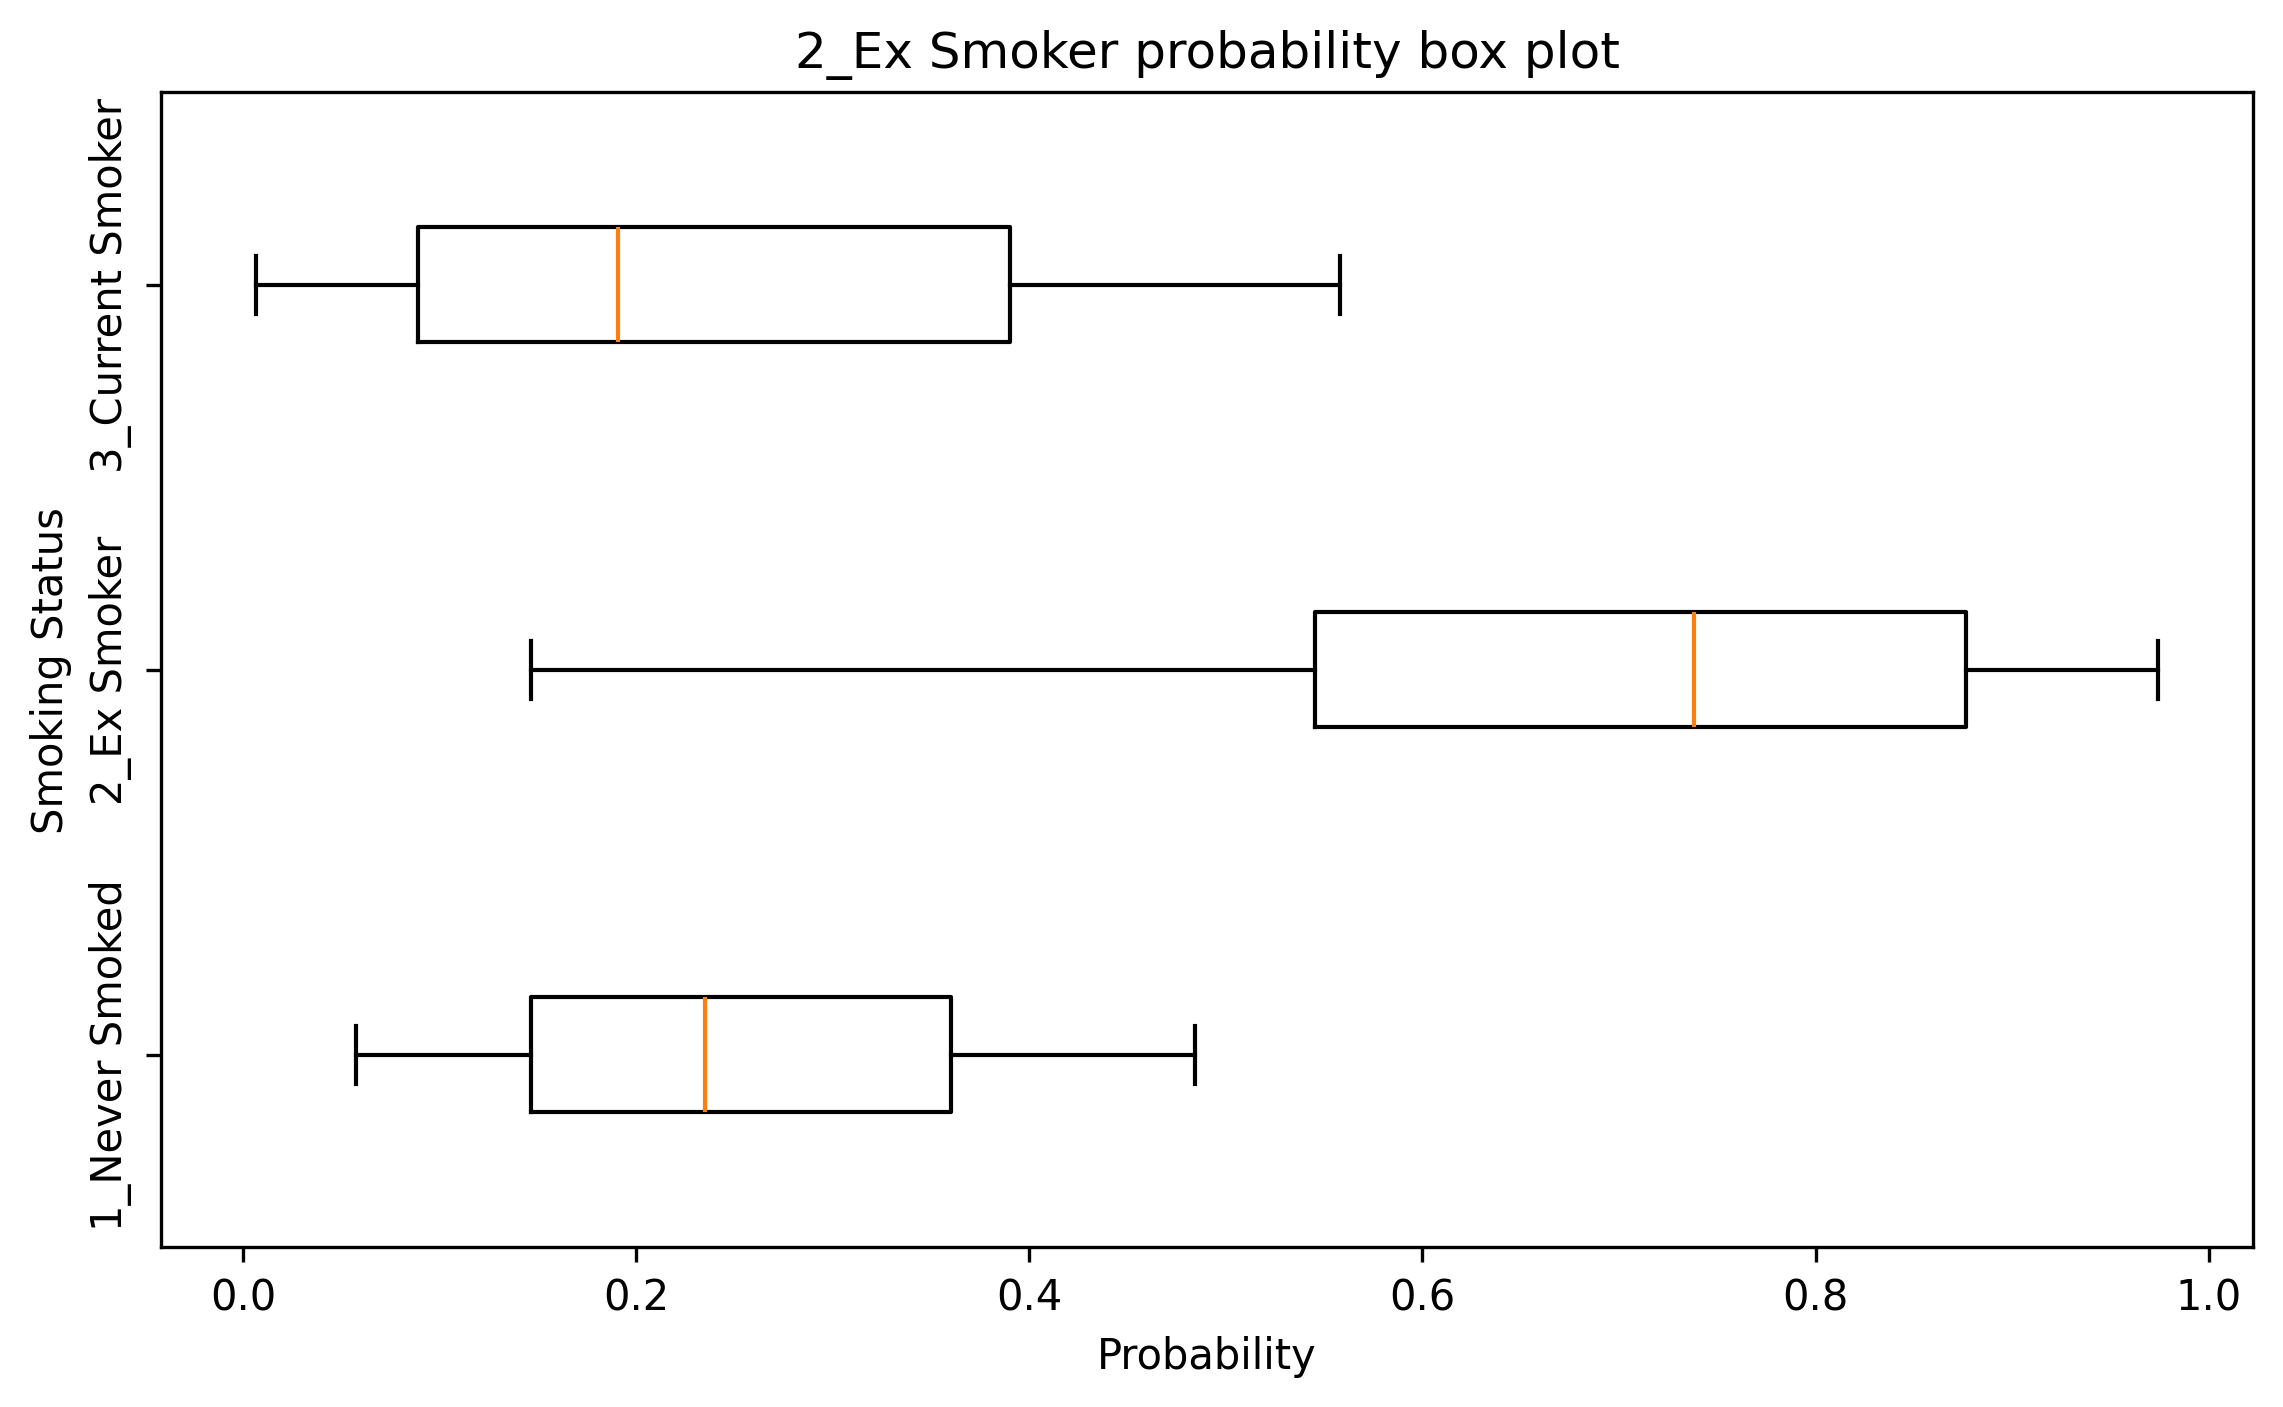
\includegraphics[width=\linewidth]{cohort1/test_boxplot_2.png}
    \end{subfigure}
    \begin{subfigure}{0.48\linewidth}
        \centering
        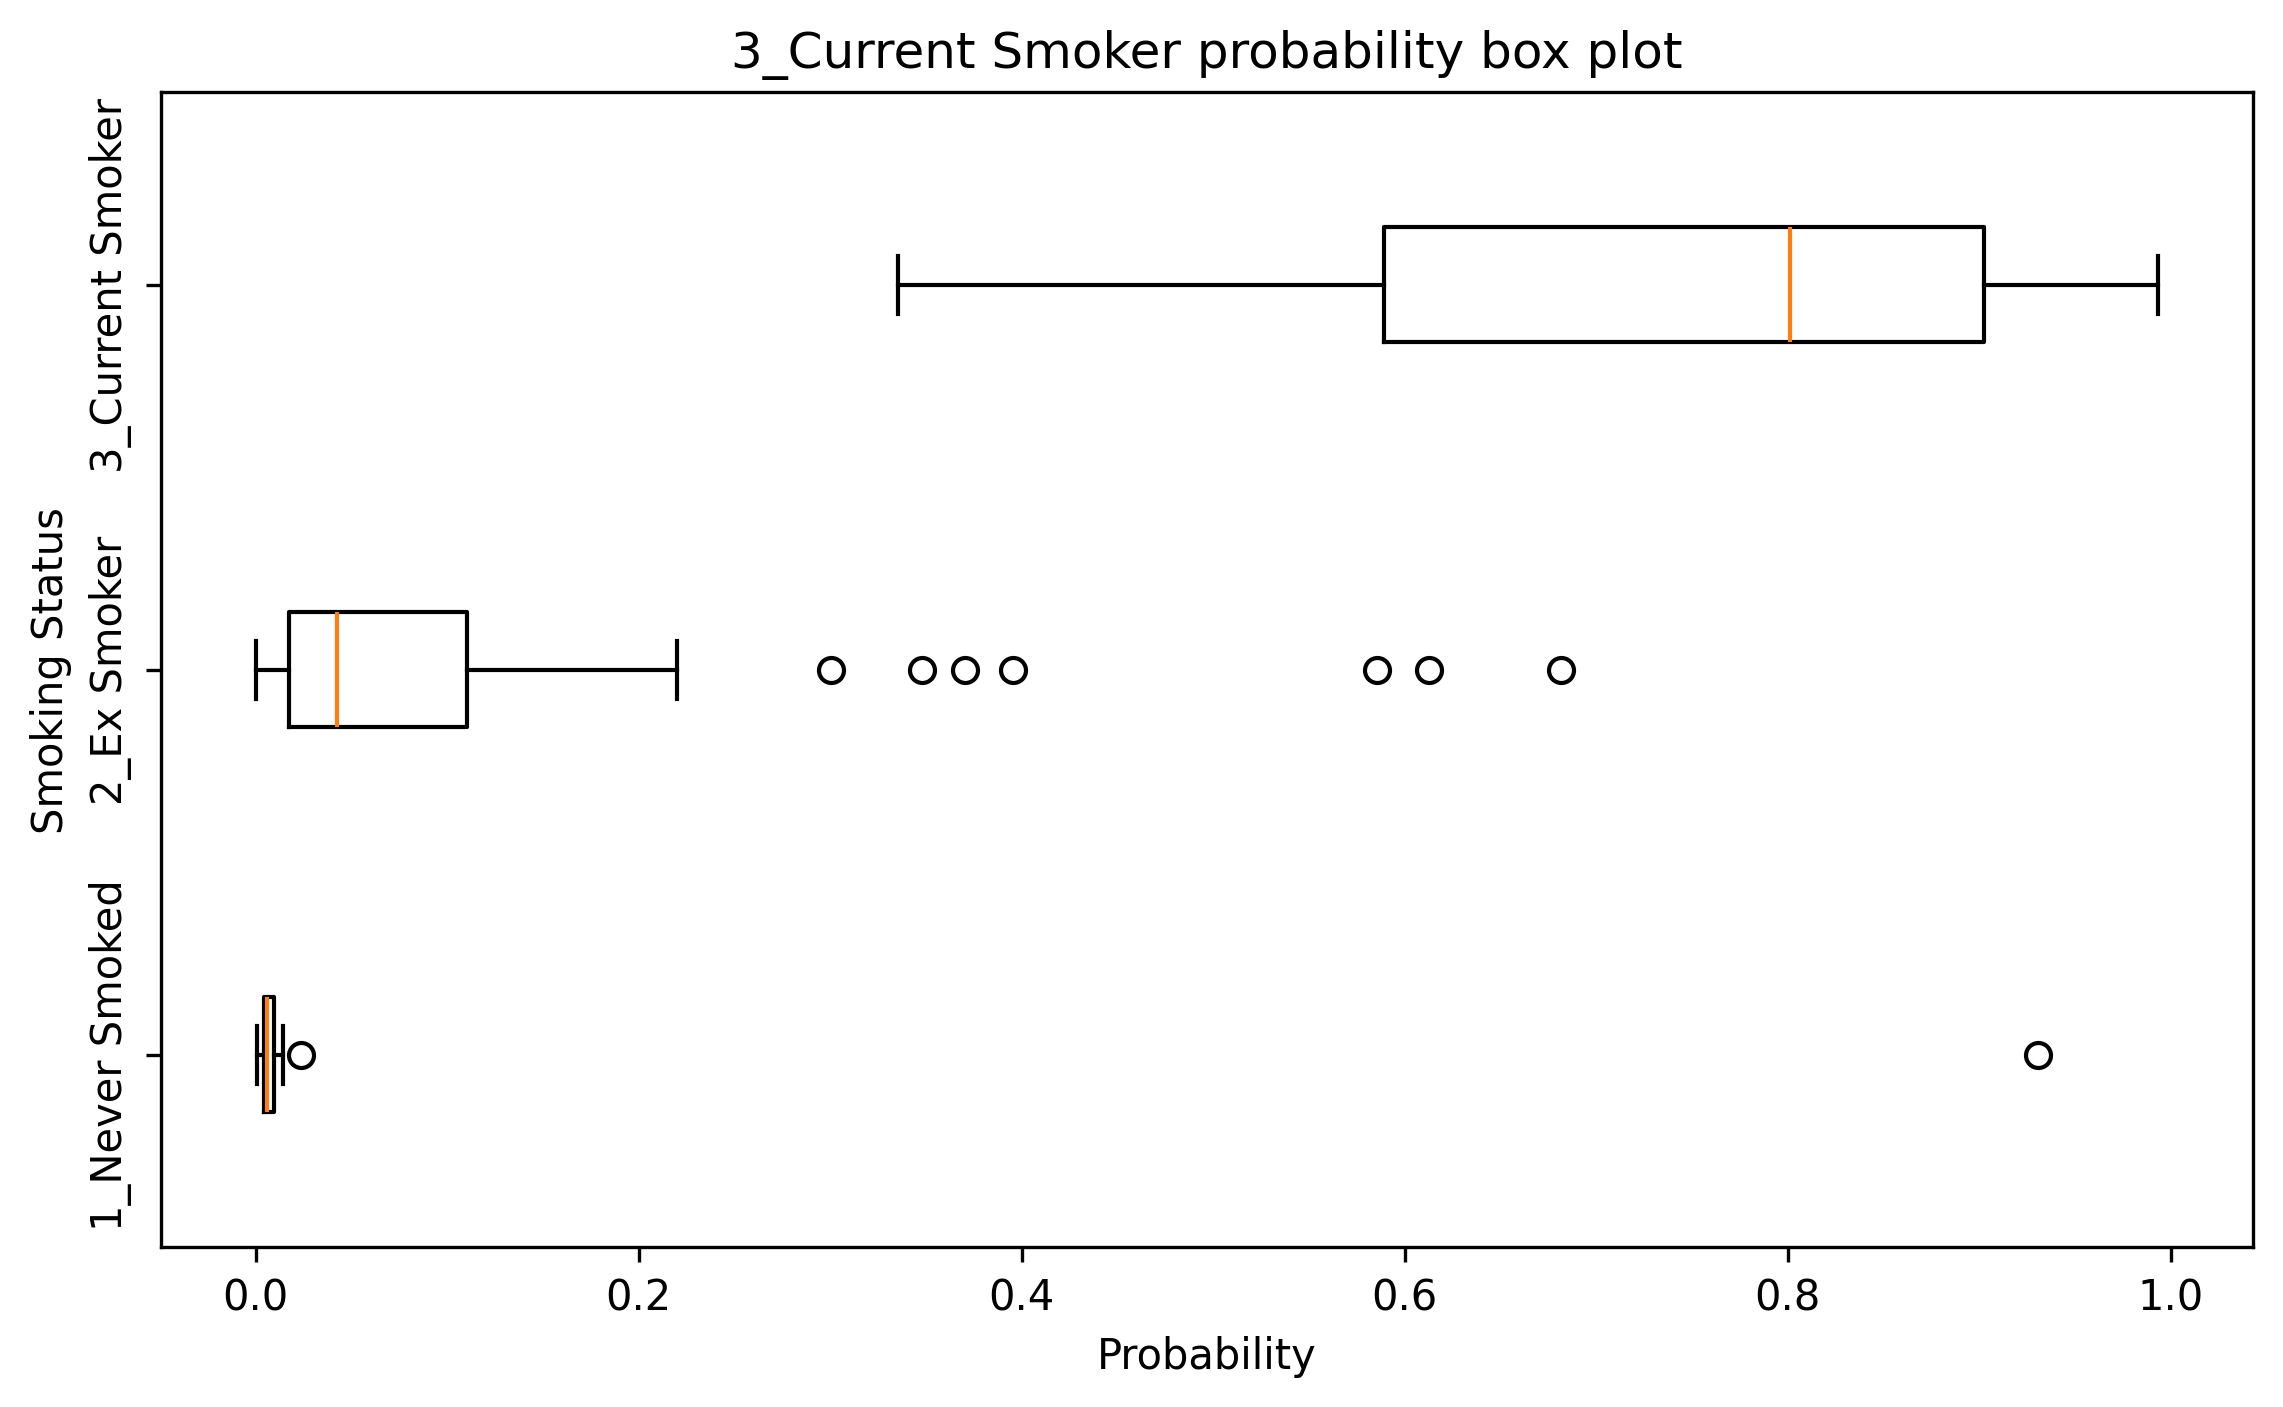
\includegraphics[width=\linewidth]{cohort1/test_boxplot_3.png}
    \end{subfigure}
    \caption[Class-specific probability box plots (Cohort 1 - Test)]{Class-specific probability box plots (Cohort 1 - Test). Each box plot shows the range of probability outputs for a given class-specific predictor, separated by class. In this cohort, each class-specific predictor assigned high probabilities to its positive class, and low probabilities to the other classes.}
    \label{fig:cohort1-boxplots}
\end{figure}

Finally, distributions of probabilities per class, per class-specific predictor, can be seen in Figure \ref{fig:cohort1-boxplots}. Here we can see each class-specific predictor generally predicted its positive class with high probability, and the two negative classes with low probability. This separation was distinct for the predictor of current-smokers and never-smokers, with little to no overlap between box plots. However, separation is less distinct for ex-smokers, as there is some overlap between the box plots of ex-smokers and the box plots of the other classes. This is perhaps unsurprising, given that ex-smokers are the intermediate class, and a biological state between current- and never-smokers.

% \textbf{Discussion points for this section:}
% \begin{itemize}
%     \item worst performance in ex-Smokers
%     \item solution: break ex smokers into two groups based on length of cessation
%     \item improve training as two different thing aren't training to be the same
%     \item this observation emphasises the need to better classifies ex smokers (biologically, they're known to not be the same (in terms of health outcomes))
% \end{itemize}

% \begin{enumerate}
%     \item Performance on Cohort 1 test set
%           \begin{itemize}
%               \item Confusion matrices
%               \item ROC diagrams
%               \item Have tabulated data with ROC diagrams
%               \item Boxplots
%           \end{itemize}
% \end{enumerate}

\newpage
\subsection{Independent cohort model performance (Cohort 2)} \label{sec:cohort2-performance}
ENSS achieved modest predictive performance on the Cohort 2 independent test dataset. The classification performance on this dataset can be seen in Figure \ref{fig:cohort2-confusion-matrix}. Out of the 984 individuals in this dataset, 271 were misclassified by the model. Per class, \SI{73}{\percent} of current-smokers and \SI{78}{\percent} of ex-smokers were correctly classified, while only \SI{0.36}{\percent} of never-smokers were correctly classified, with \SI{0.62}{\percent} of never-smokers being confused for ex-smokers. Compared to the performance in Cohort 1, there was a clear decrease in predictive accuracy in Cohort 2.

The model's ability to separate classes was also evaluated. Macro-averaged OvO ROC curves for the entire model can be seen in Figure \ref{fig:cohort2-macro-rocs}. These were generated by aggregating OvO ROC curves of the class-specific predictors, seen in Figure \ref{fig:cohort2-initial-rocs}. The model achieved macro-averaged OvO ROC-AUCs of: 0.971 for separating never-smokers from current-smokers, 0.859 for separating ex-smokers from current-smokers, and 0.686 for separating never-smokers from ex-smokers. Comparing the performance in Cohort 1 to Cohort 2, we can see the model maintained the ability to discriminate never-smokers from current-smokers, but the ability to separate ex-smokers from current-smokers was only good, and the ability to separate never-smokers from ex-smokers was poor.

Finally, distributions of probabilities per class, per class-specific predictor, can be seen in Figure \ref{fig:cohort2-boxplots}. As seen in the ROC curves, the model was able to separate current-smokers from the other two classes, predicting high probabilities in the current-smoker class-specific predictor, and low probabilities in the other two predictors. However, we can see between the never-smoker and ex-smoker class-specific predictor box plots there was significant overlap, leading to misclassification and confusion between these two classes.

\begin{figure}[p]
    \centering
    \begin{subfigure}{0.49\linewidth}
        \centering
        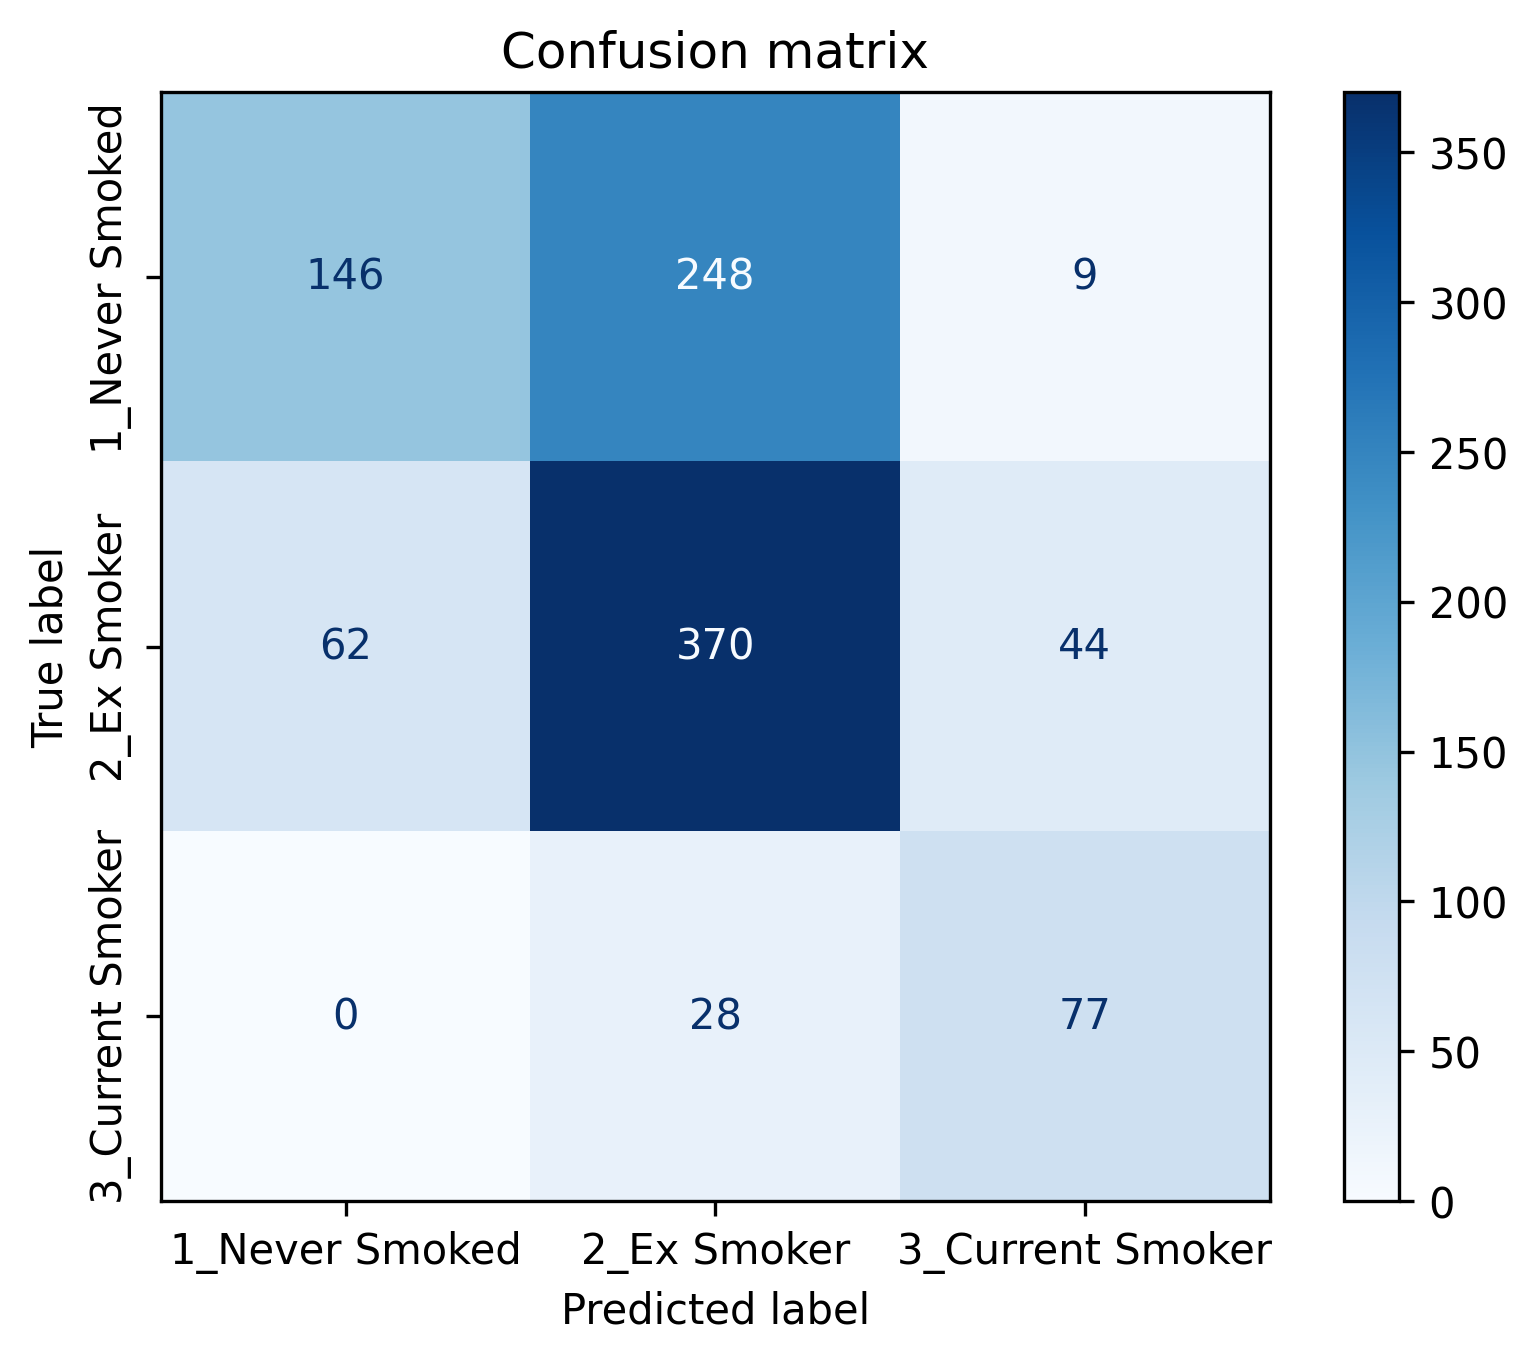
\includegraphics[width=\linewidth]{cohort2/test_confusion_matrix.png}
        \caption{Counts}
    \end{subfigure}
    \hfill
    \begin{subfigure}{0.49\linewidth}
        \centering
        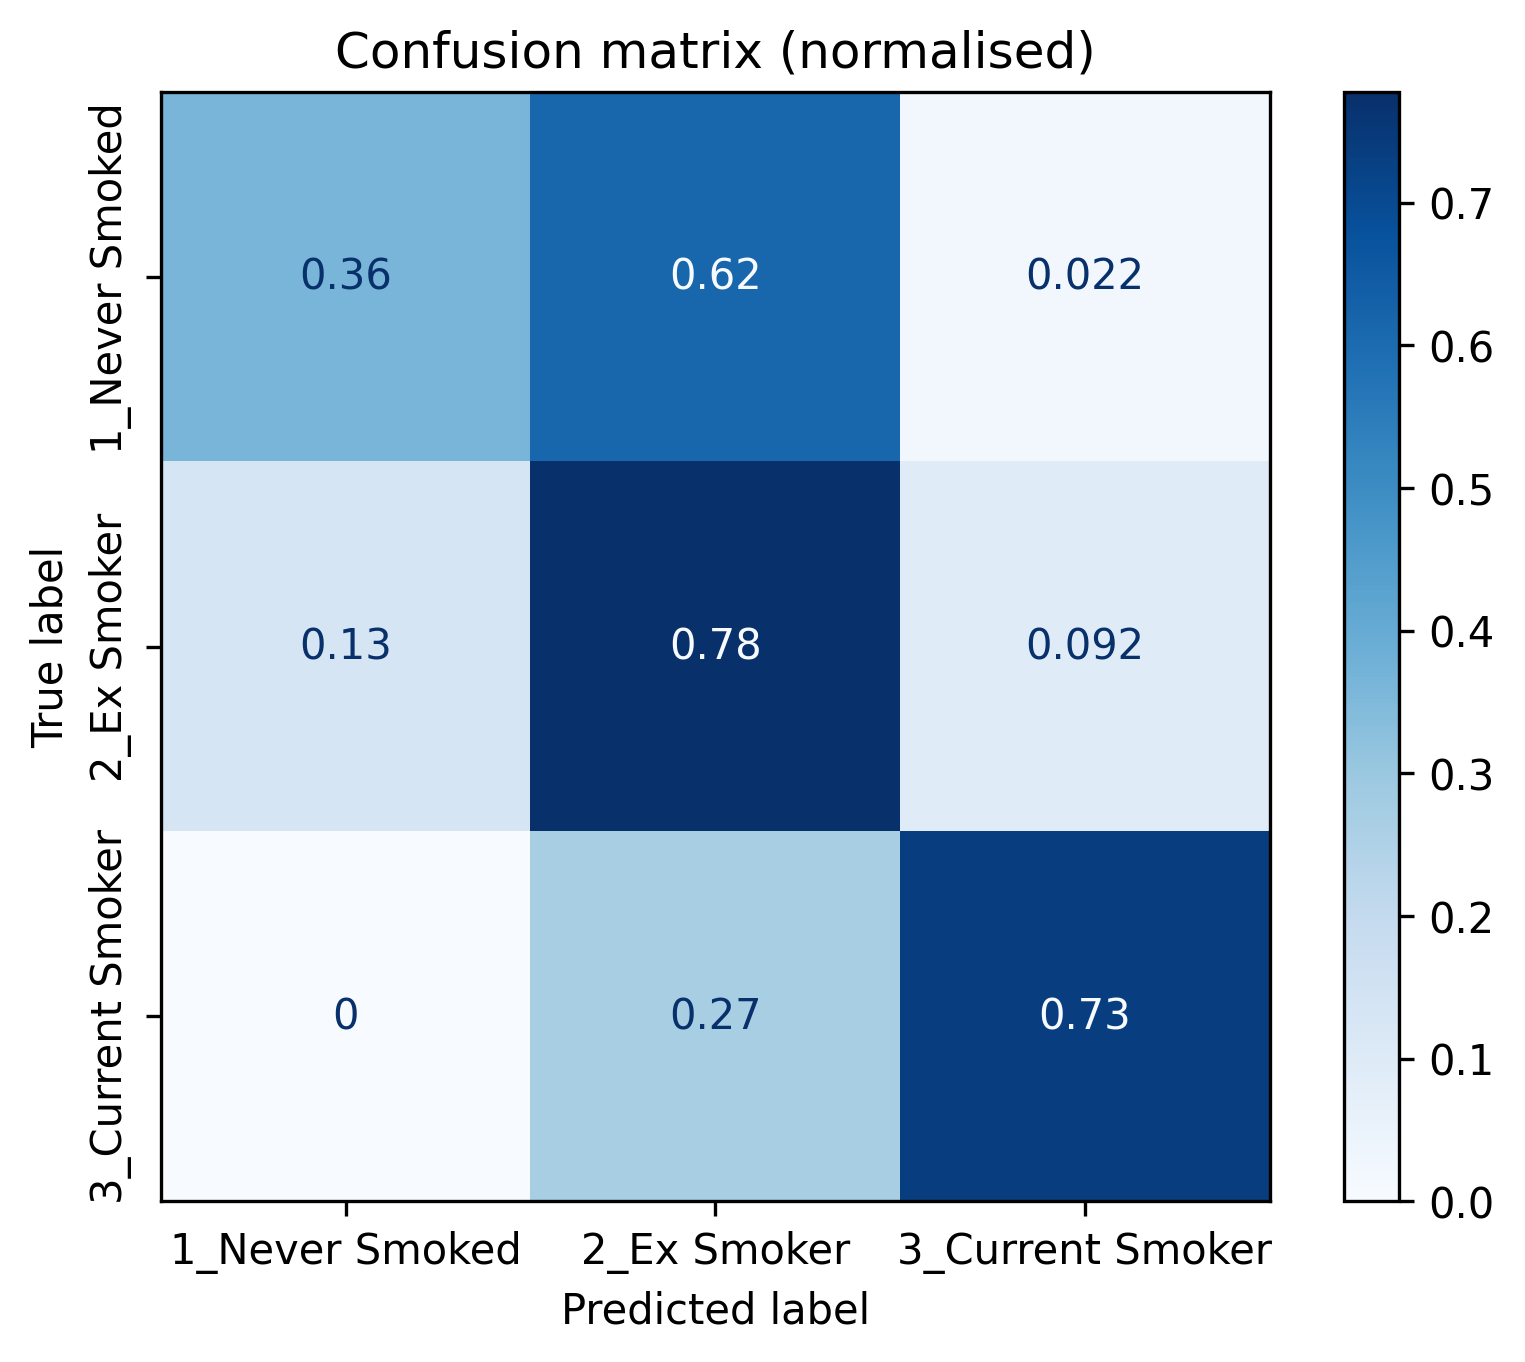
\includegraphics[width=\linewidth]{cohort2/test_confusion_matrix_normalised.png}
        \caption{Percentages}
    \end{subfigure}
    \caption[Confusion matrices (Cohort 2)]{Confusion matrices (Cohort 2). The model classified ex- and never-smokers with moderate accuracy in this cohort, but misclassified most never-smokers as ex-smokers.}
    \label{fig:cohort2-confusion-matrix}
\end{figure}

\begin{figure}[p]
    \centering
    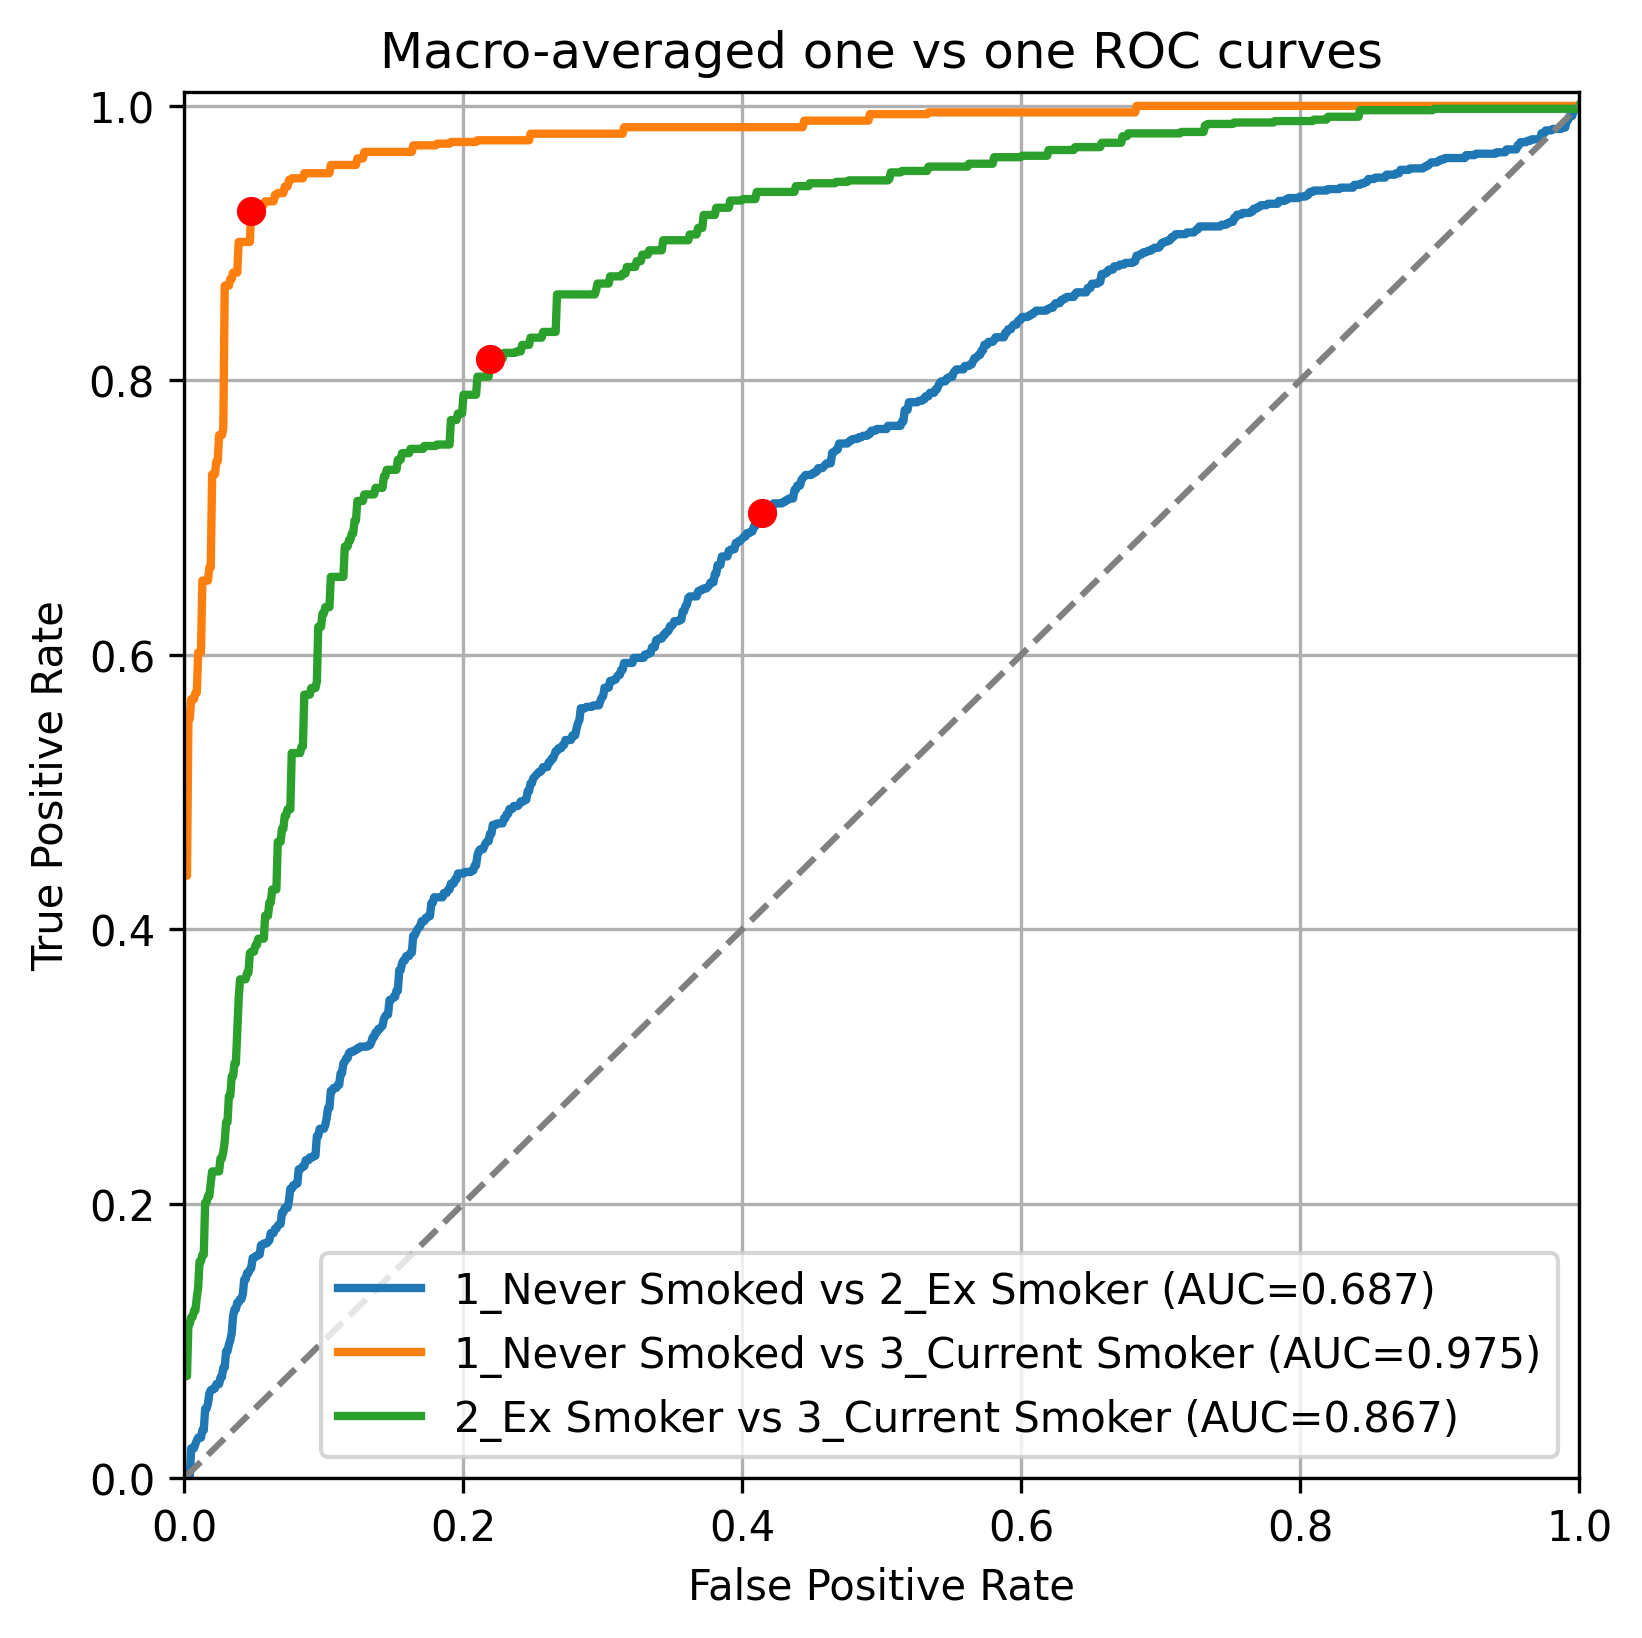
\includegraphics[width=0.7\linewidth]{cohort2/test_macro_ovo_roc.png}
    \caption[Macro-averaged ROC curves (Cohort 2)]{Macro-averaged ROC curves (Cohort 2). Each curve aggregates the two relevant class-specific predictors into a single ROC curve, giving a single curve which evaluates the entire model's performance separating two classes. The model's separation of never- and current-smokers was excellent in this cohort, while separation of ex- and current-smokers was good, and separation of never- and ex-smokers was poor.}
    \label{fig:cohort2-macro-rocs}
\end{figure}

\begin{figure}[p]
    \centering
    \begin{subfigure}{0.46\linewidth}
        \centering
        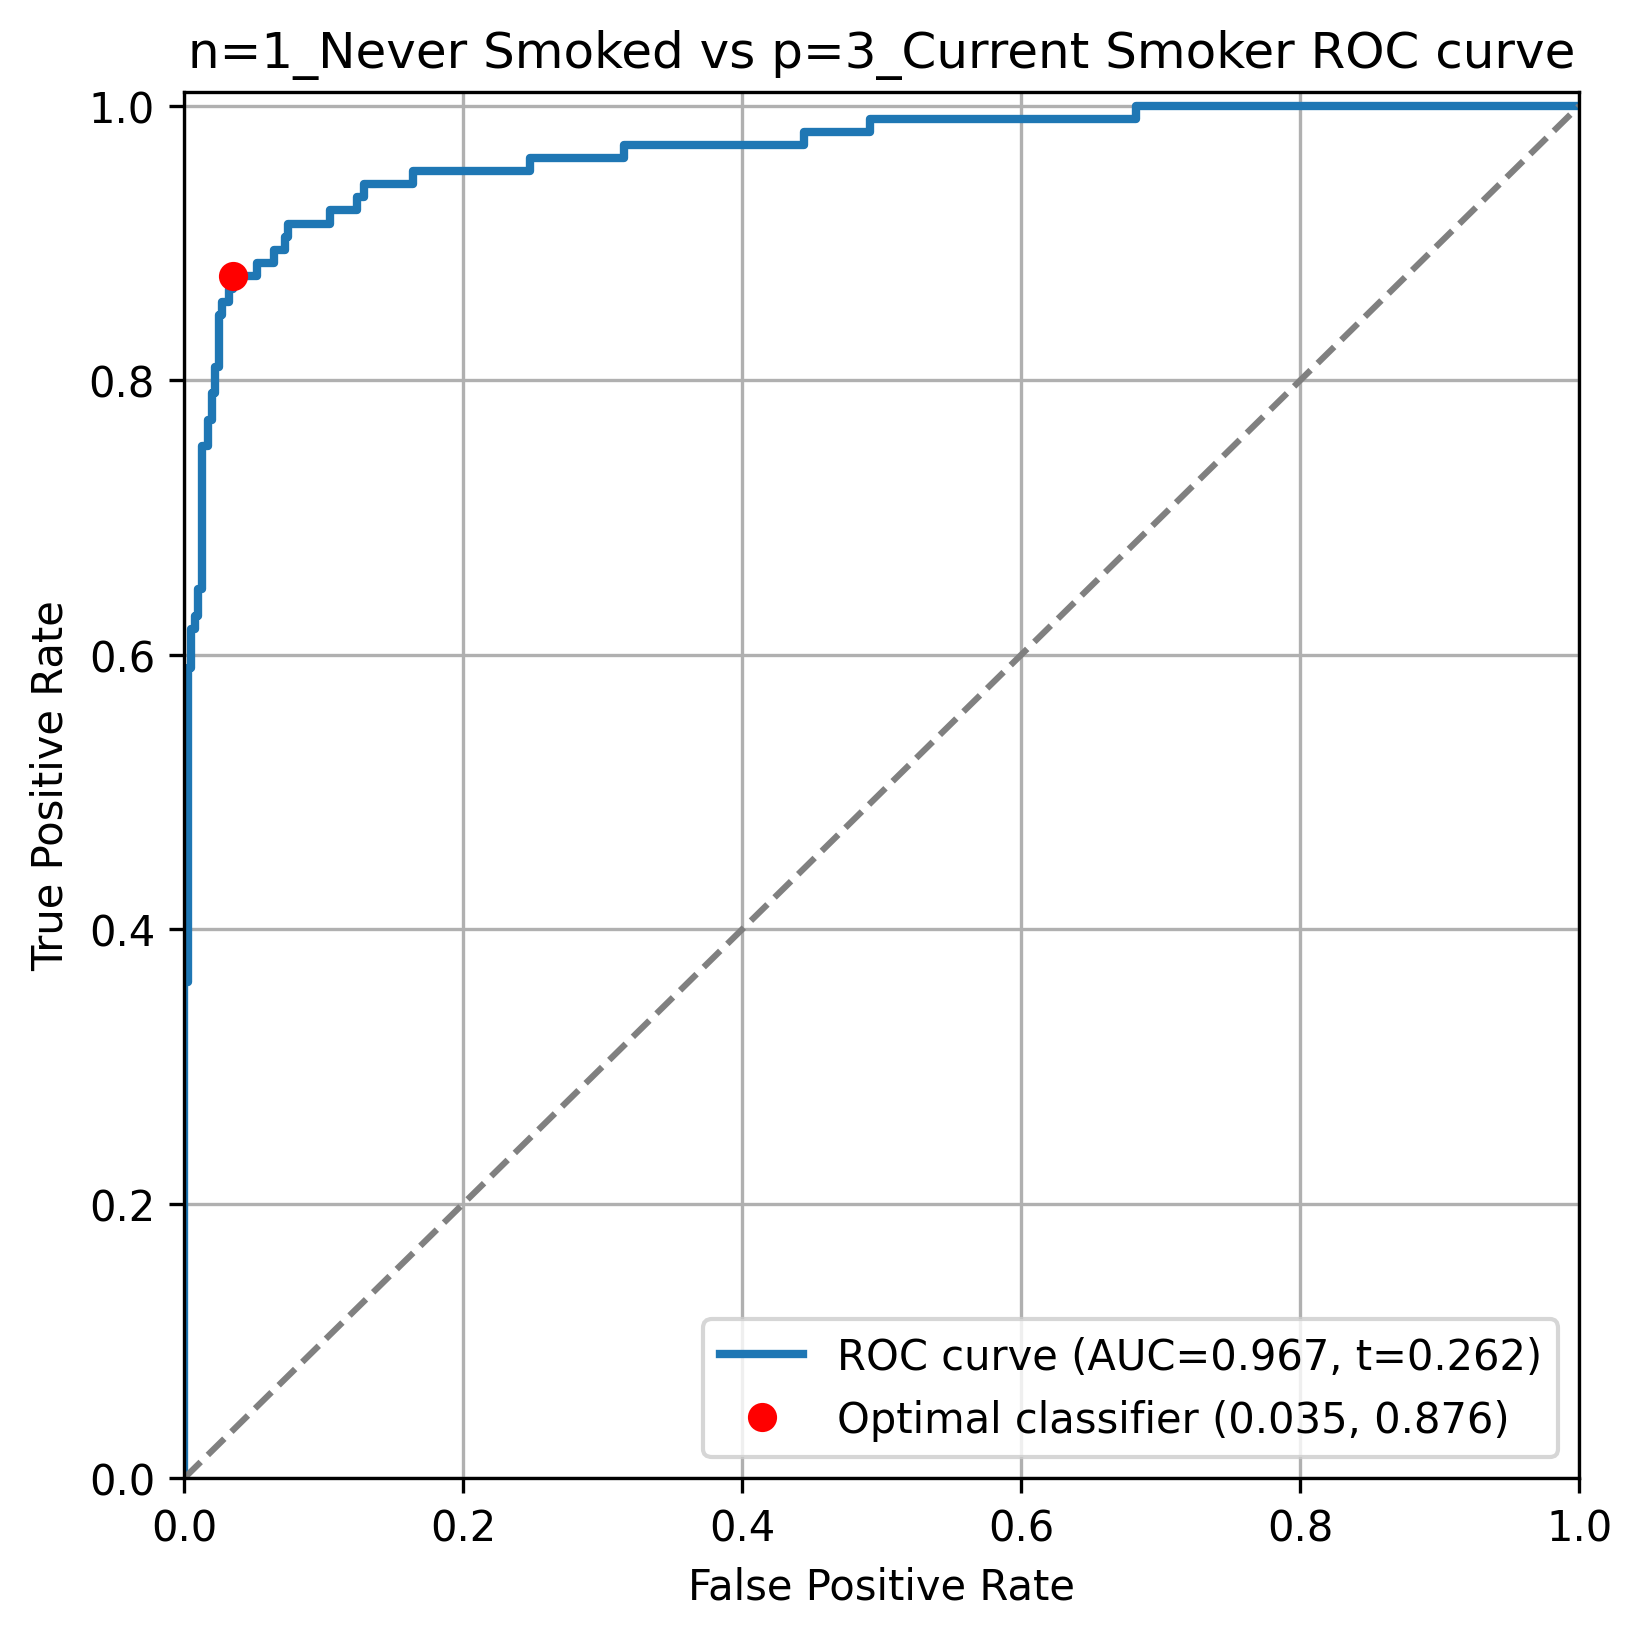
\includegraphics[width=\linewidth]{cohort2/test_1v3_roc.png}
    \end{subfigure}
    \hspace{4mm}
    \begin{subfigure}{0.46\linewidth}
        \centering
        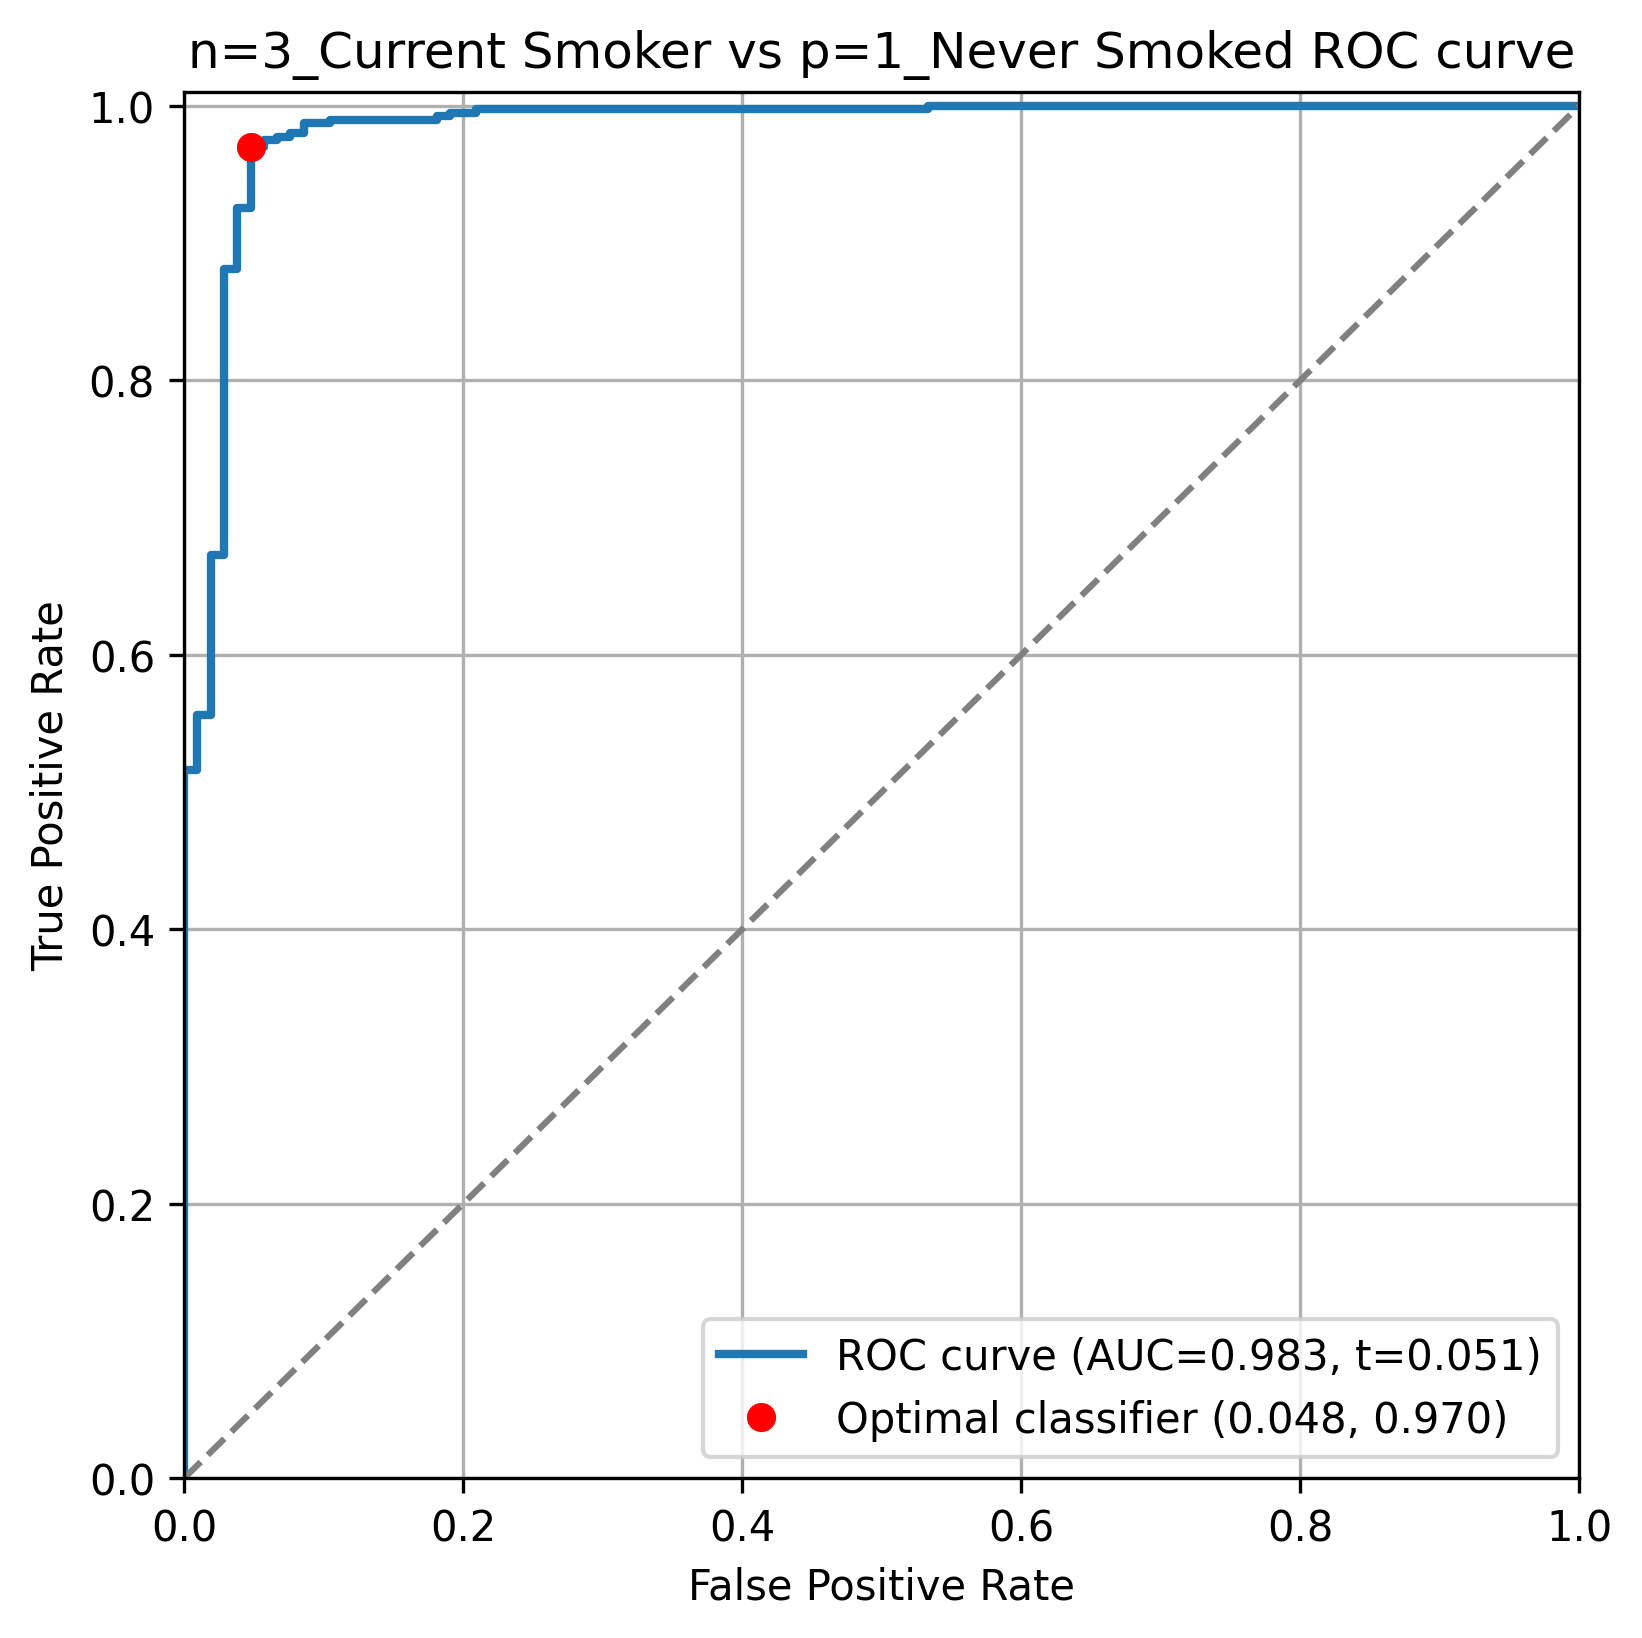
\includegraphics[width=\linewidth]{cohort2/test_3v1_roc.png}
    \end{subfigure}

    \begin{subfigure}{0.46\linewidth}
        \centering
        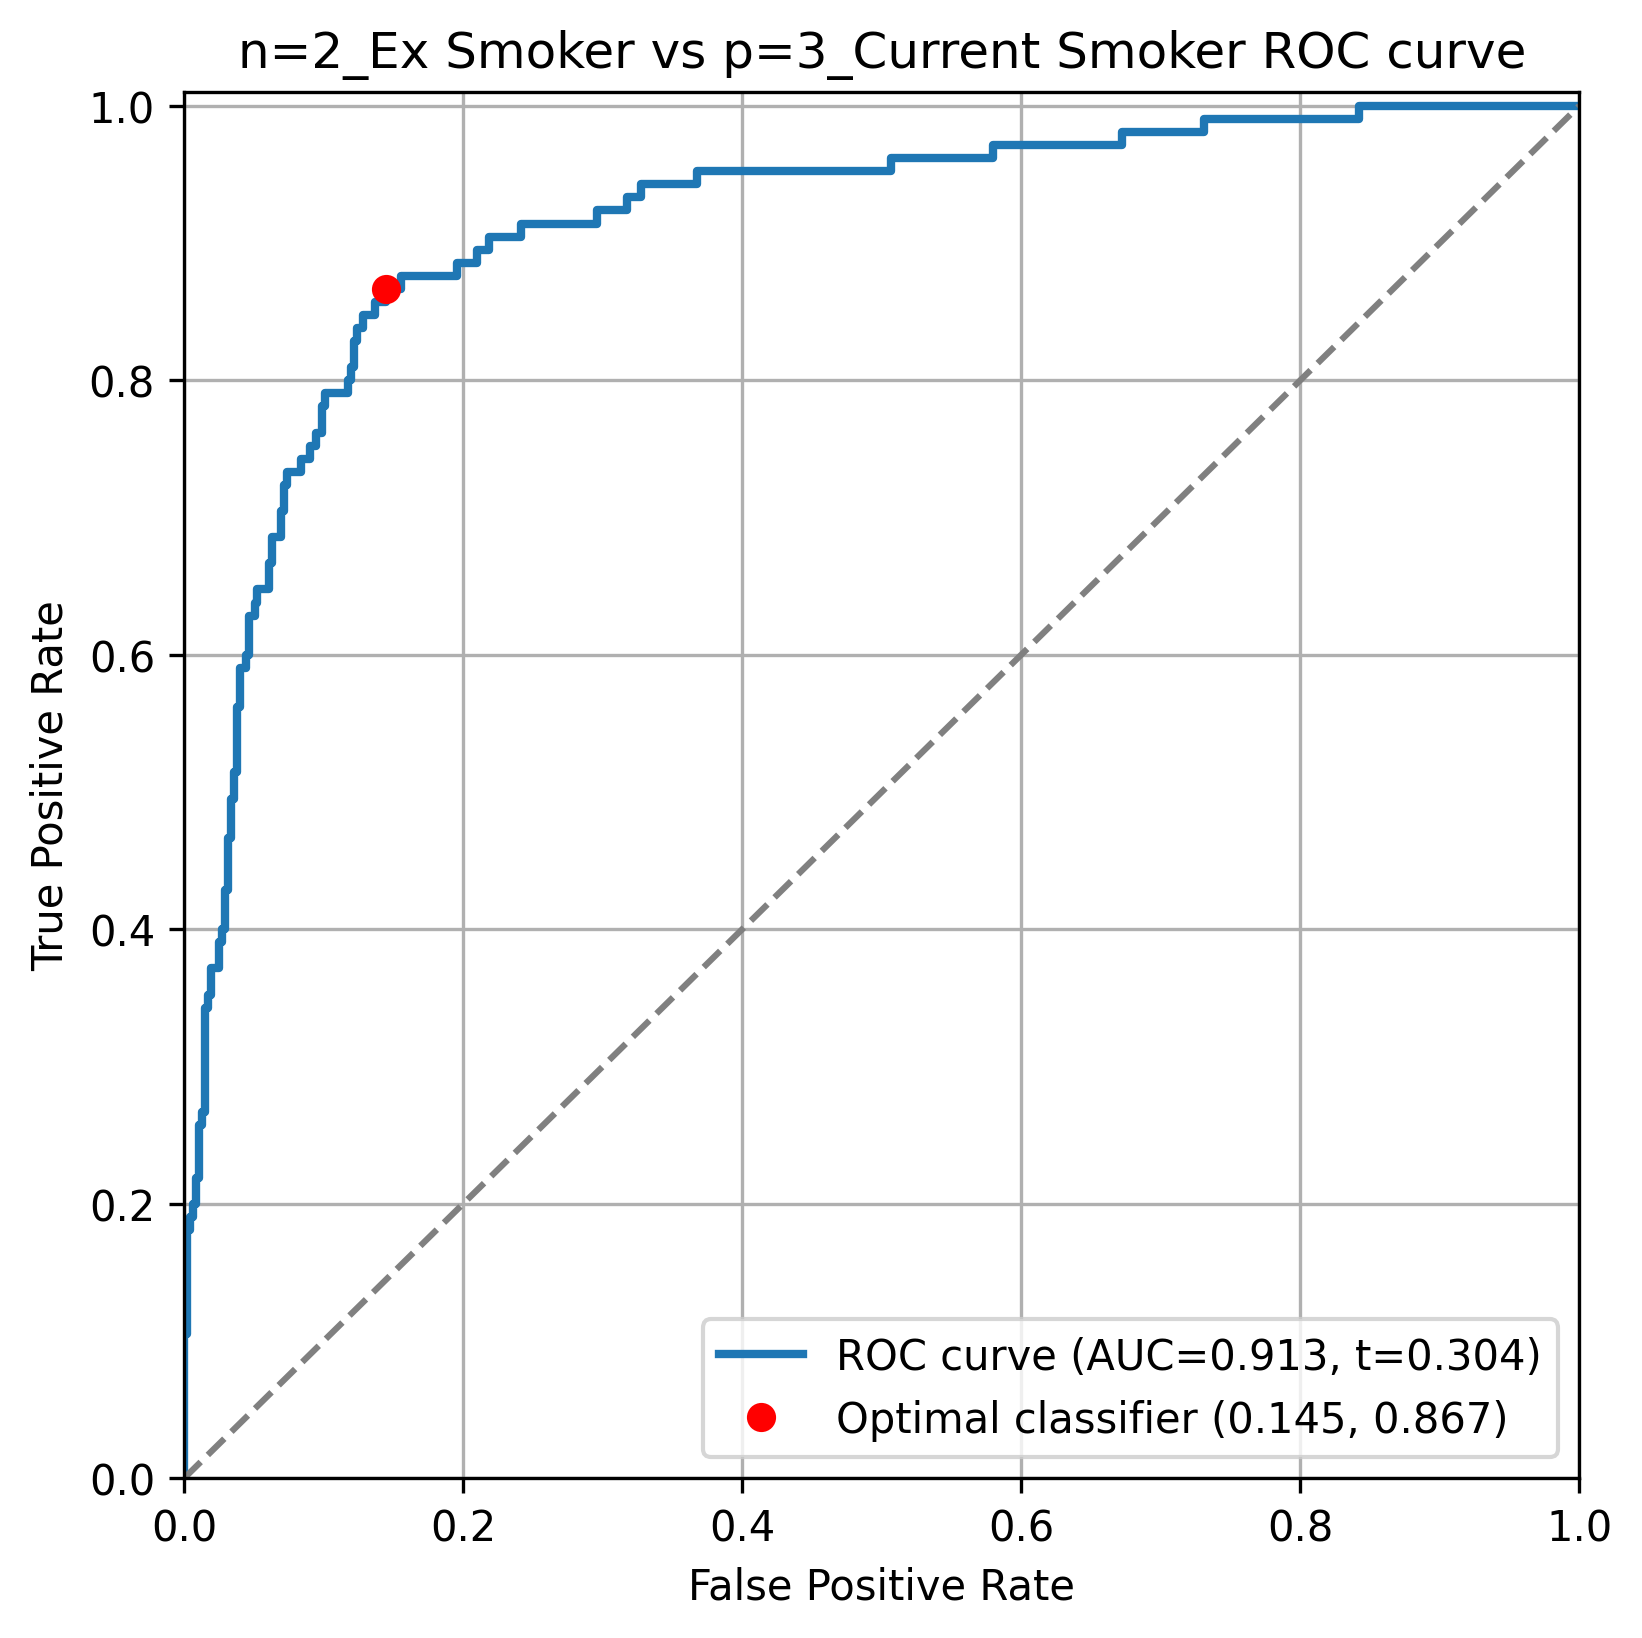
\includegraphics[width=\linewidth]{cohort2/test_2v3_roc.png}
    \end{subfigure}
    \hspace{4mm}
    \begin{subfigure}{0.46\linewidth}
        \centering
        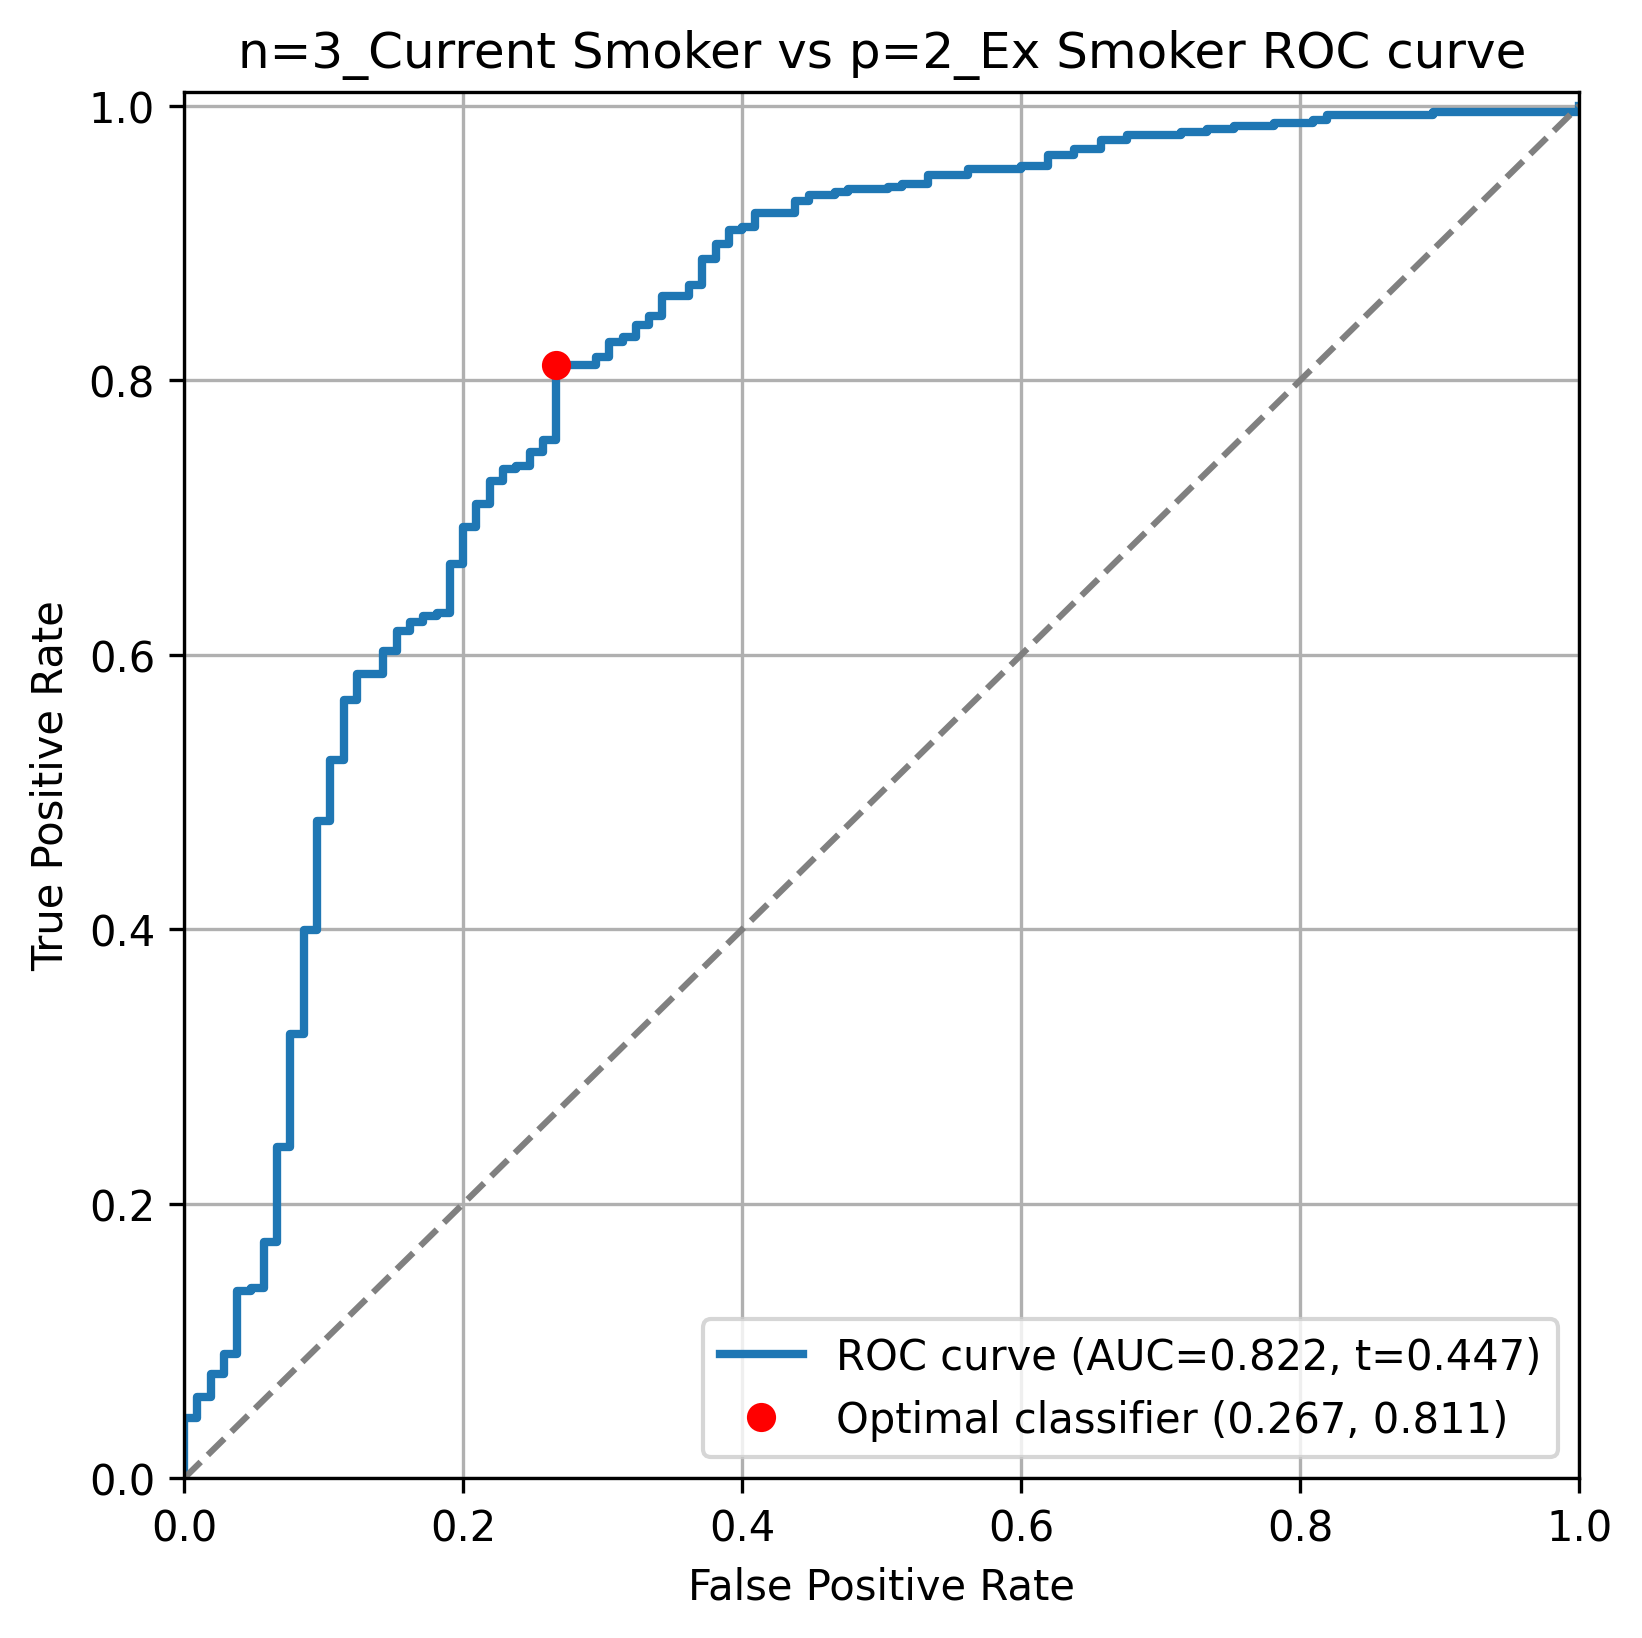
\includegraphics[width=\linewidth]{cohort2/test_3v2_roc.png}
    \end{subfigure}

    \begin{subfigure}{0.46\linewidth}
        \centering
        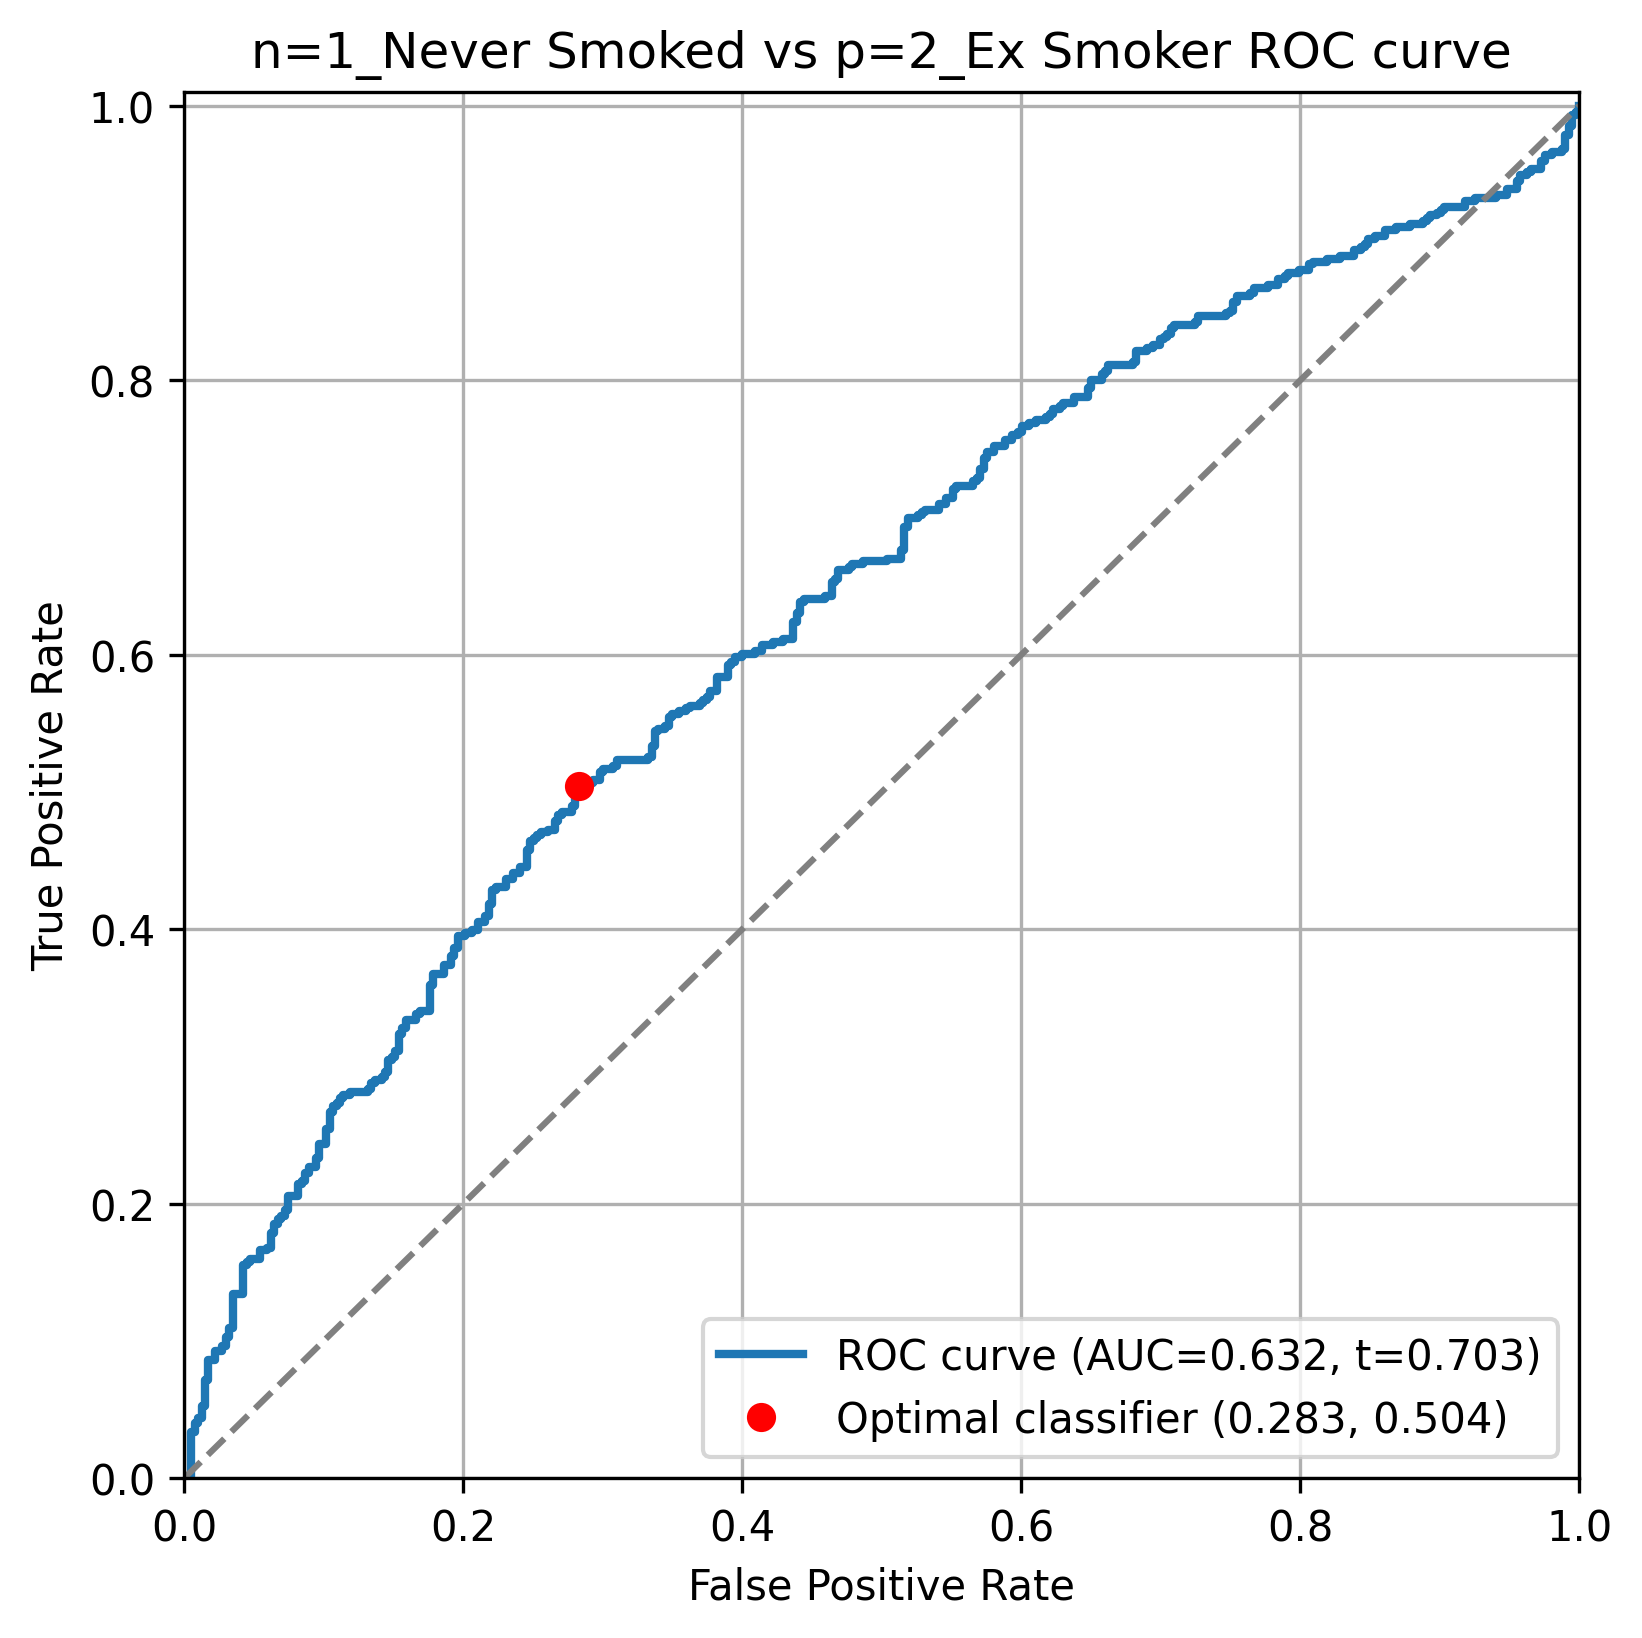
\includegraphics[width=\linewidth]{cohort2/test_1v2_roc.png}
    \end{subfigure}
    \hspace{4mm}
    \begin{subfigure}{0.46\linewidth}
        \centering
        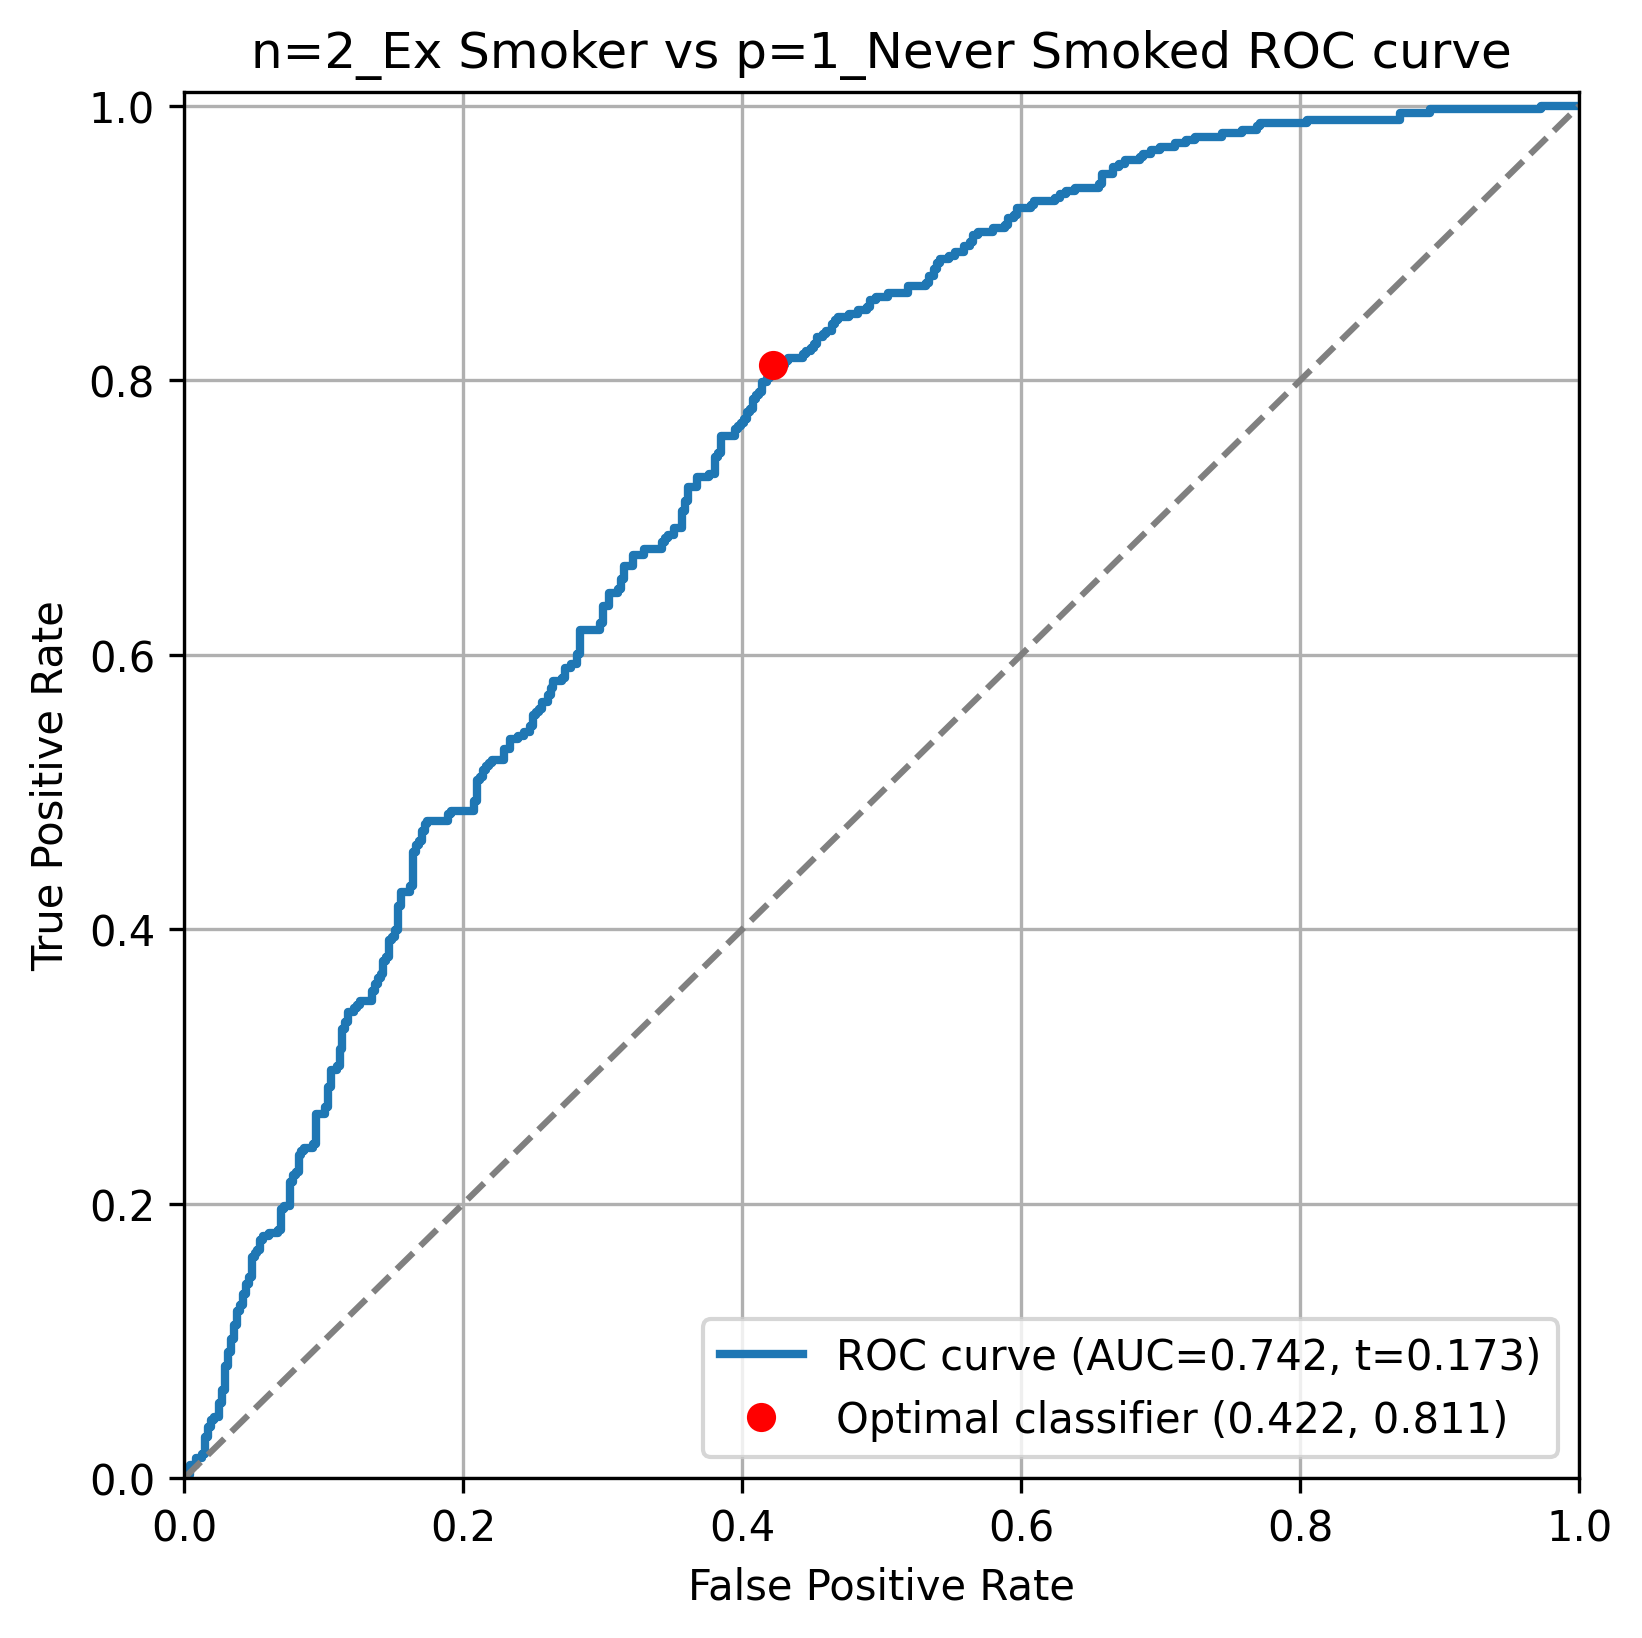
\includegraphics[width=\linewidth]{cohort2/test_2v1_roc.png}
    \end{subfigure}
    \caption[Class-specific predictor ROC curves (Cohort 2)]{OvO class-specific predictor ROC curves (Cohort 2). Each curve shows a single class-specific predictor's ability to separate two classes, using the probability outputs for the given predictor. The predictor used for each curve corresponds to the positive class. Separation of each pair of classes varied in this cohort, with class-specific predictors achieving excellent performance for never vs current, excellent to good performance for ex vs current, and poor to acceptable performance for never vs ex.}
    \label{fig:cohort2-initial-rocs}
\end{figure}

\begin{figure}[tb]
    \centering
    \begin{subfigure}{0.48\linewidth}
        \centering
        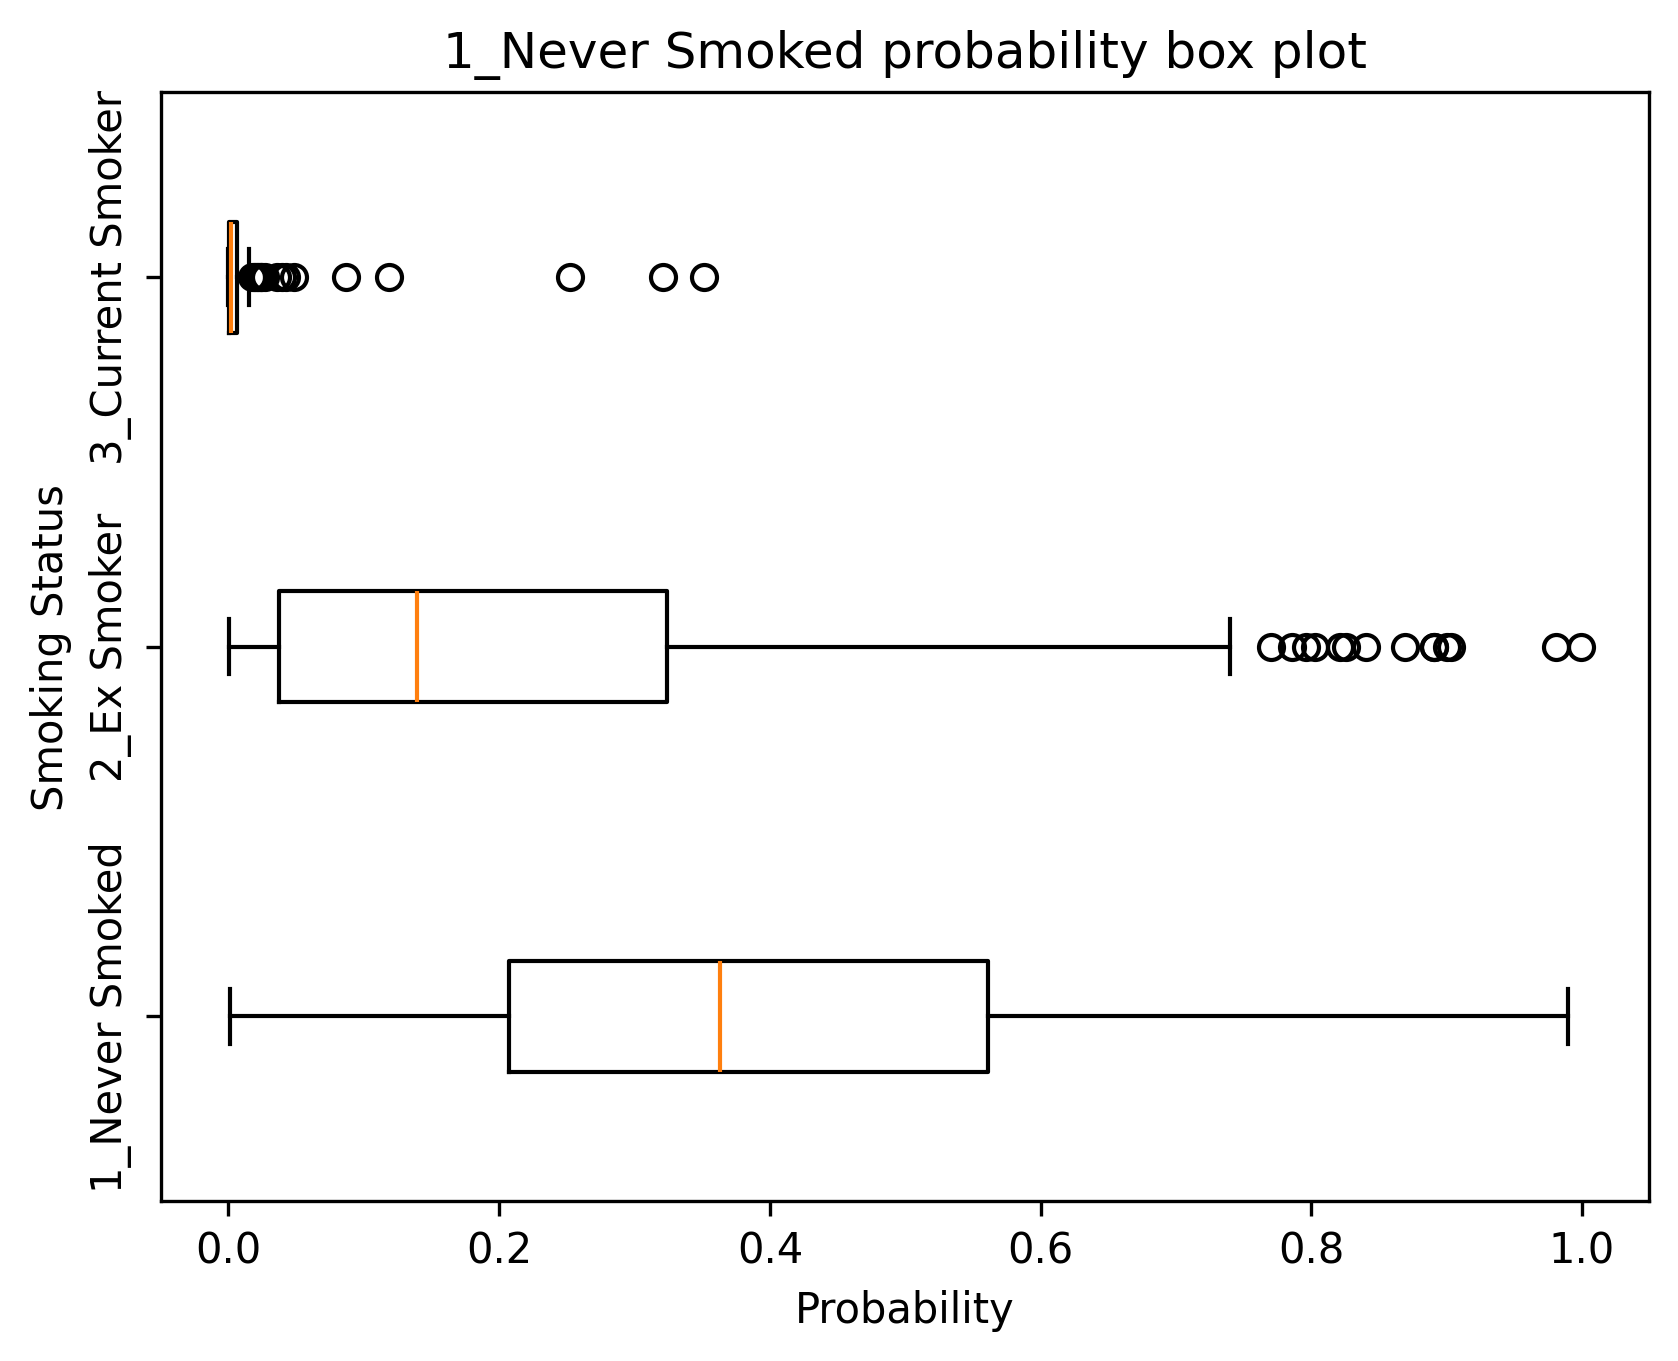
\includegraphics[width=\linewidth]{cohort2/test_boxplot_1.png}
    \end{subfigure}
    \hfill
    \begin{subfigure}{0.48\linewidth}
        \centering
        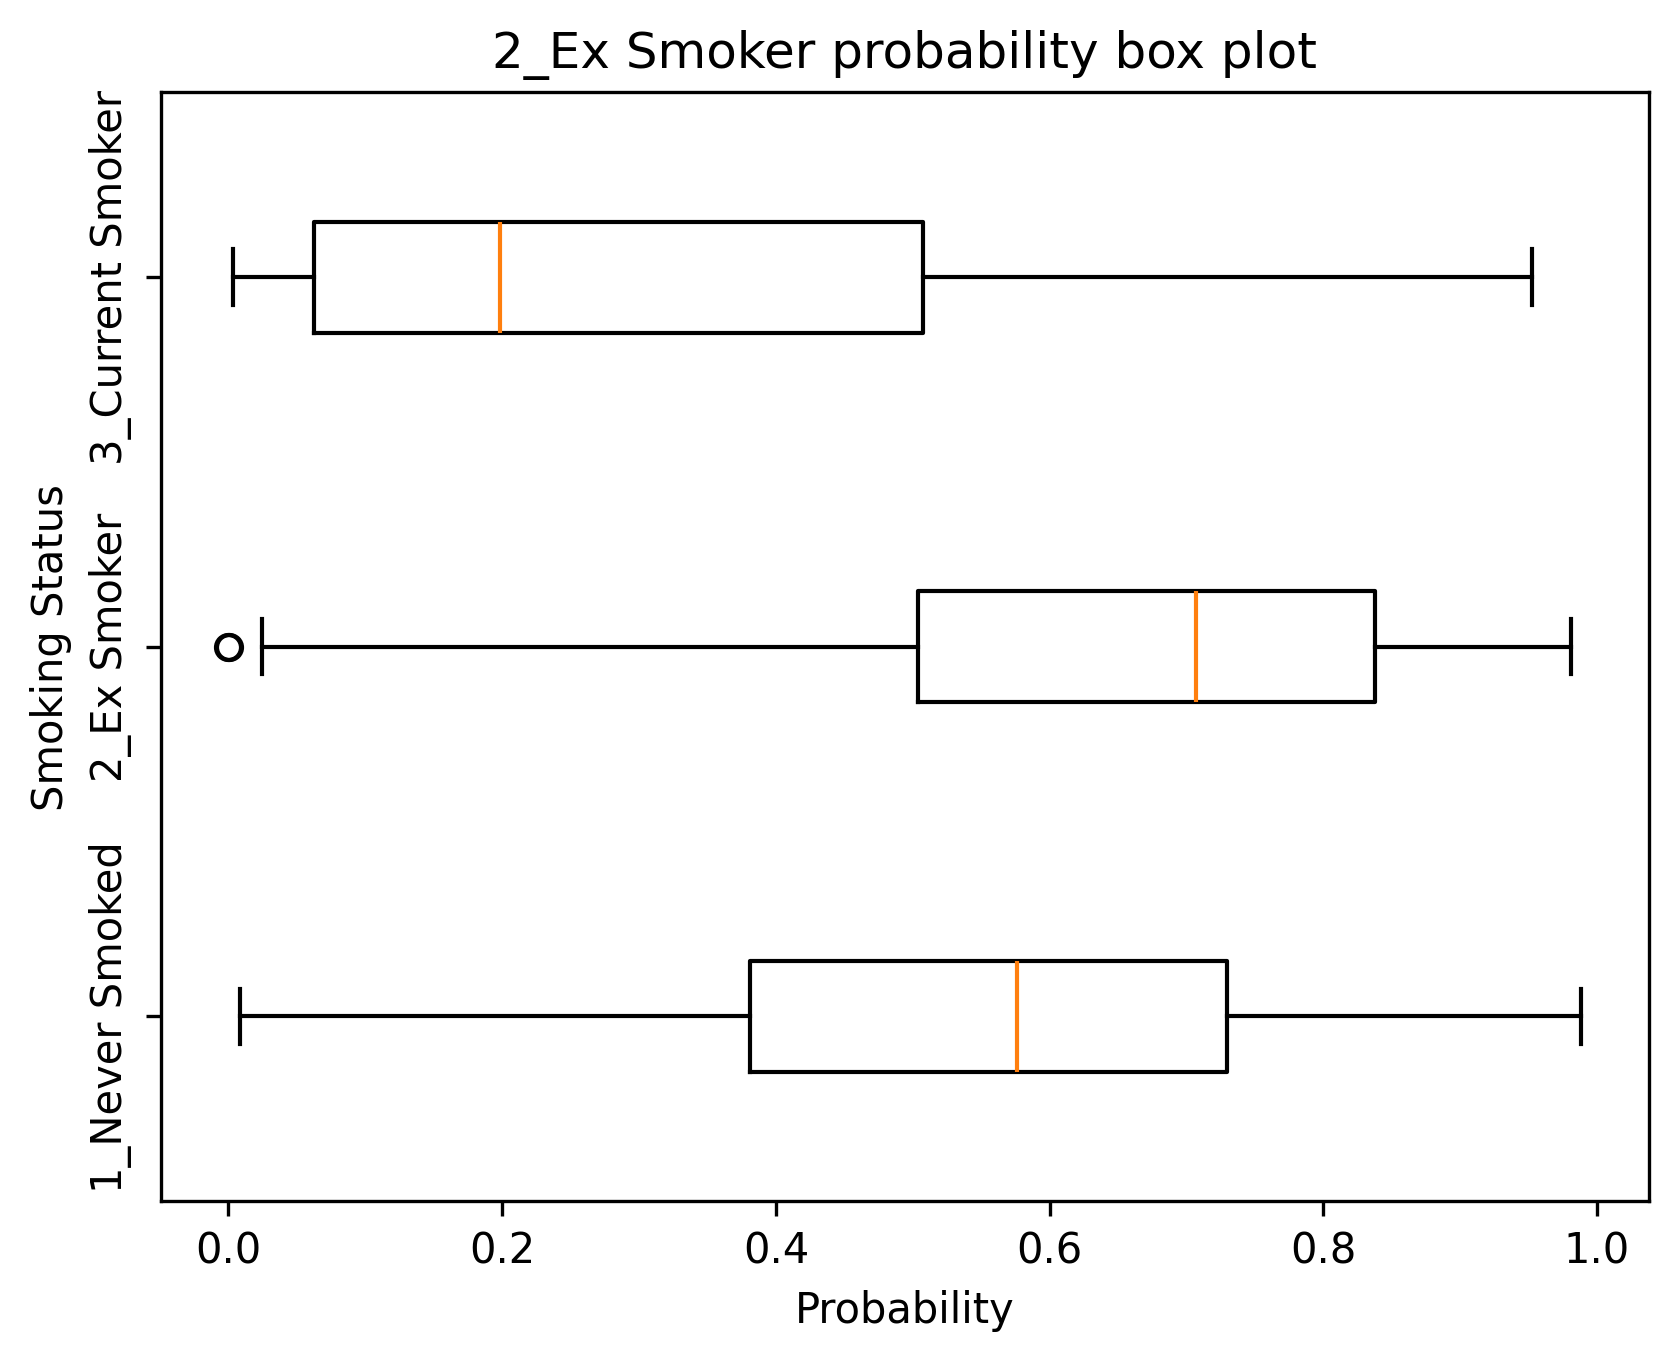
\includegraphics[width=\linewidth]{cohort2/test_boxplot_2.png}
    \end{subfigure}
    \begin{subfigure}{0.48\linewidth}
        \centering
        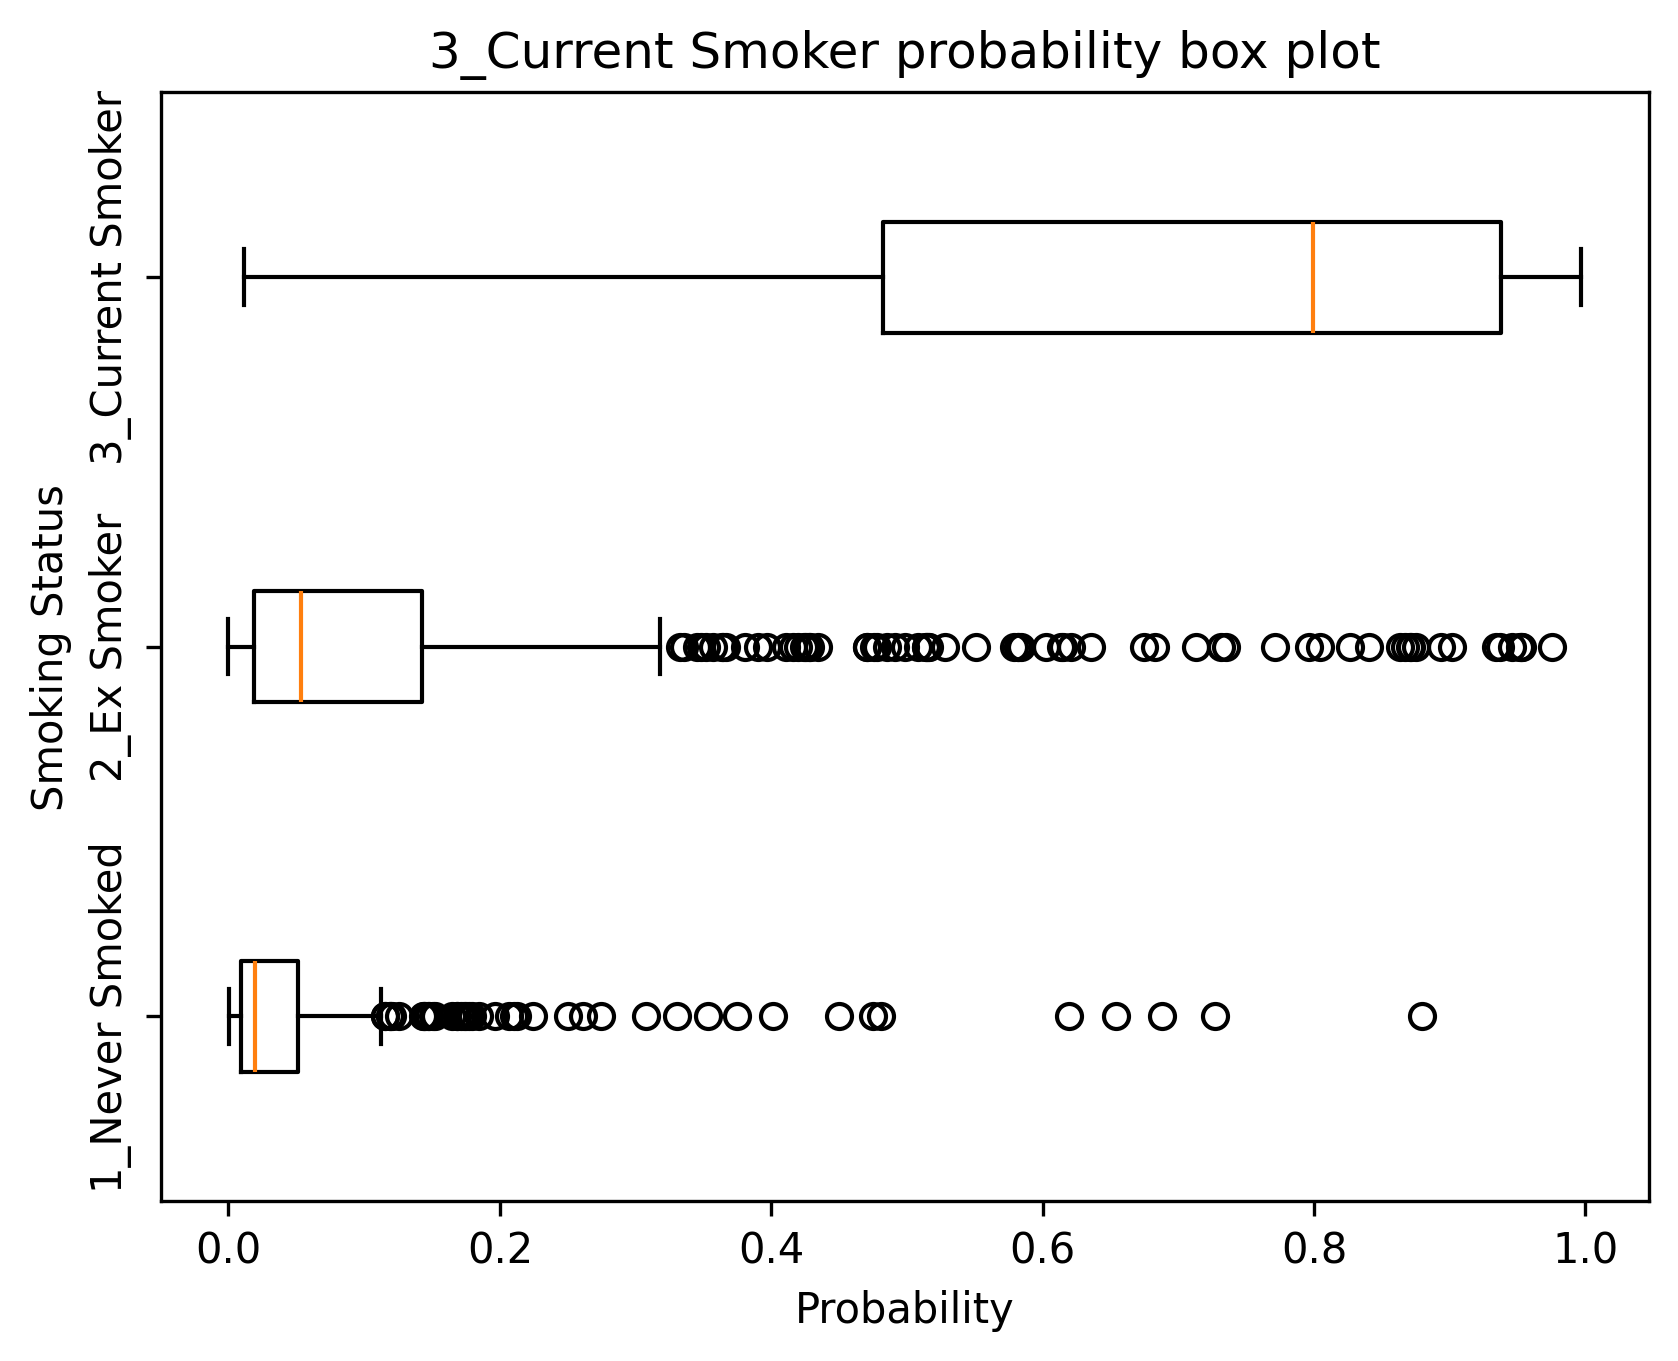
\includegraphics[width=\linewidth]{cohort2/test_boxplot_3.png}
    \end{subfigure}
    \caption[Class-specific probability box plots (Cohort 2)]{Class-specific probability box plots (Cohort 2). Each box plot shows the range of probability outputs for a given class-specific predictor, separated by class. In this cohort, probabilities were correctly assigned by the current-smoker class-specific predictor, but both the never- and ex-smoker class-specific predictors had significant overlap in the distributions of their probabilities.}
    \label{fig:cohort2-boxplots}
\end{figure}

\newpage

\subsubsection{Separating by sex}

\begin{figure}[p]
    \centering
    \begin{subfigure}{0.45\linewidth}
        \centering
        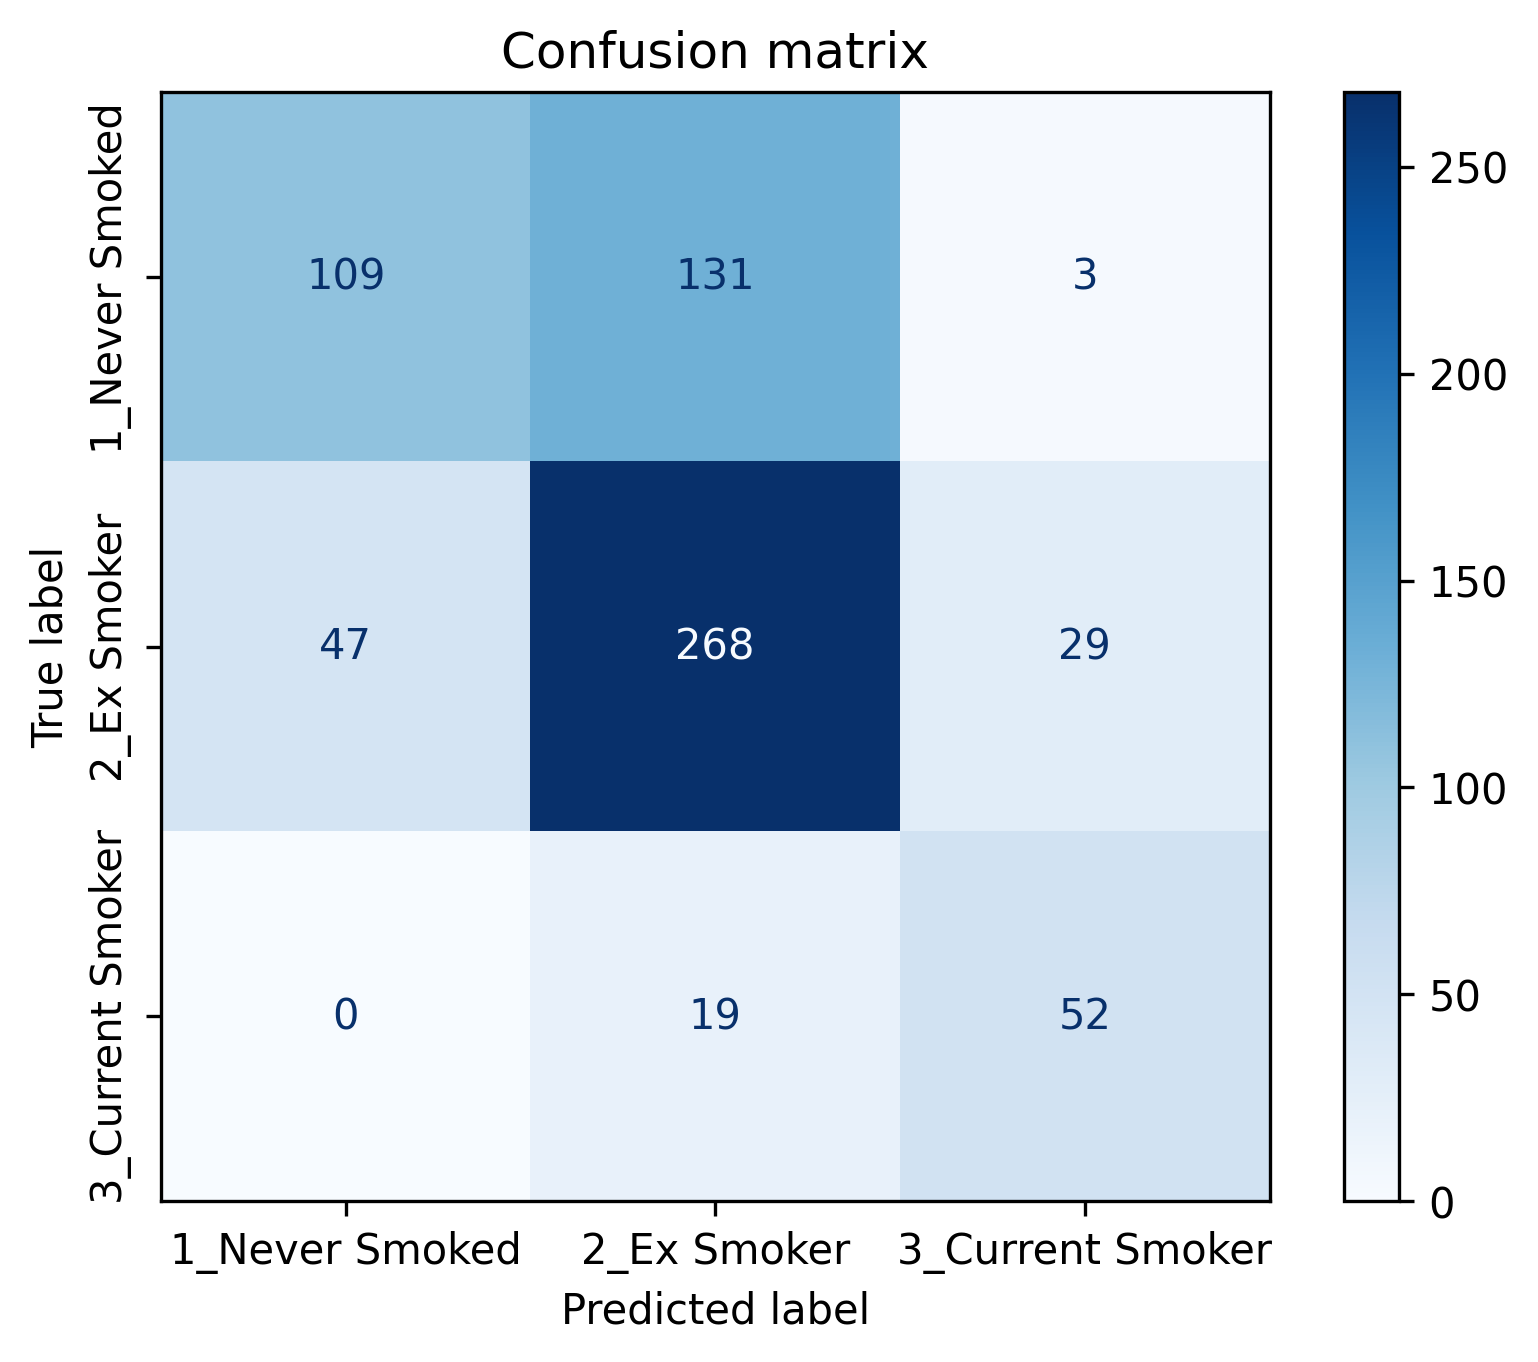
\includegraphics[width=\linewidth]{cohort2/male_only/test_confusion_matrix.png}
        \caption{Counts}
    \end{subfigure}
    \hspace{4mm}
    \begin{subfigure}{0.45\linewidth}
        \centering
        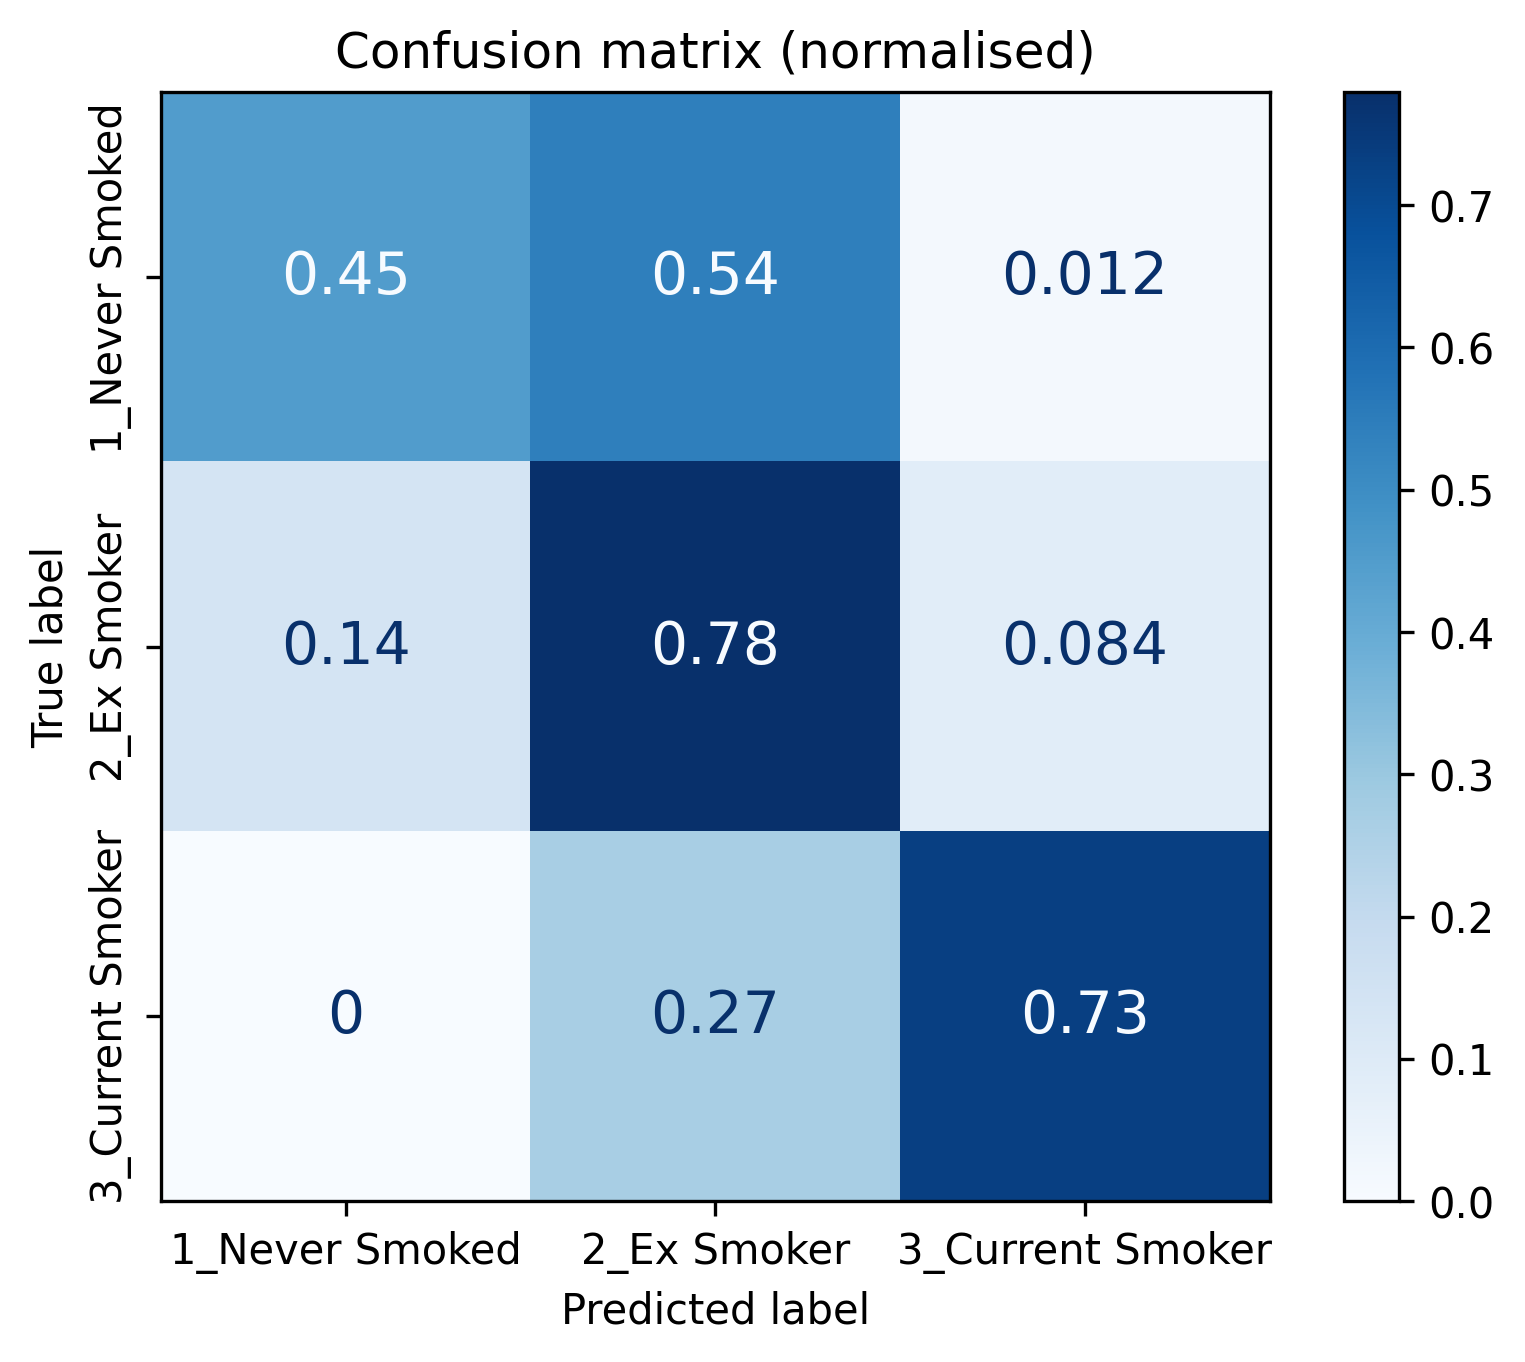
\includegraphics[width=\linewidth]{cohort2/male_only/test_confusion_matrix_normalised.png}
        \caption{Percentages}
    \end{subfigure}
    \caption[Confusion matrices (Cohort 2, male only)]{Confusion matrices (Cohort 2, male only)}
    \label{fig:male-only-confusion-matrix}
\end{figure}

\begin{figure}[p]
    \centering
    \begin{subfigure}{0.45\linewidth}
        \centering
        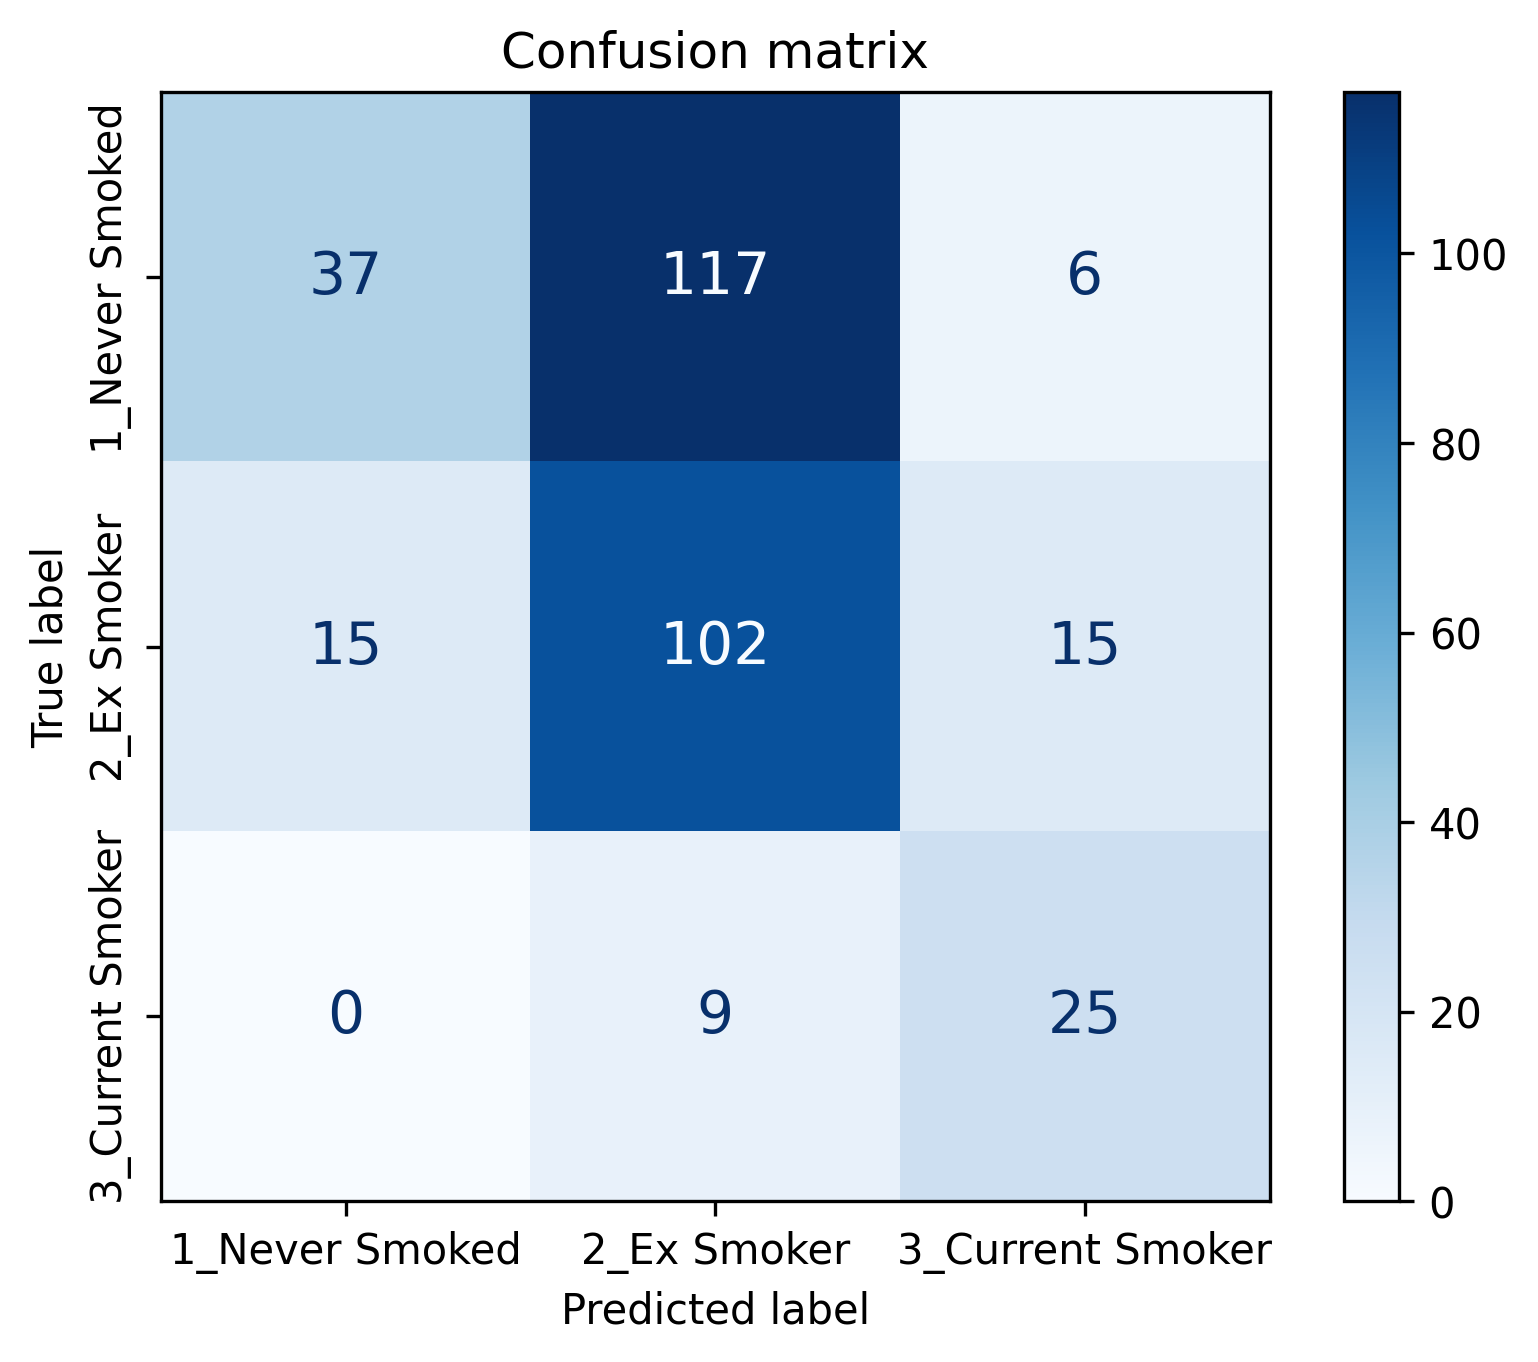
\includegraphics[width=\linewidth]{cohort2/female_only/test_confusion_matrix.png}
        \caption{Counts}
    \end{subfigure}
    \hspace{4mm}
    \begin{subfigure}{0.45\linewidth}
        \centering
        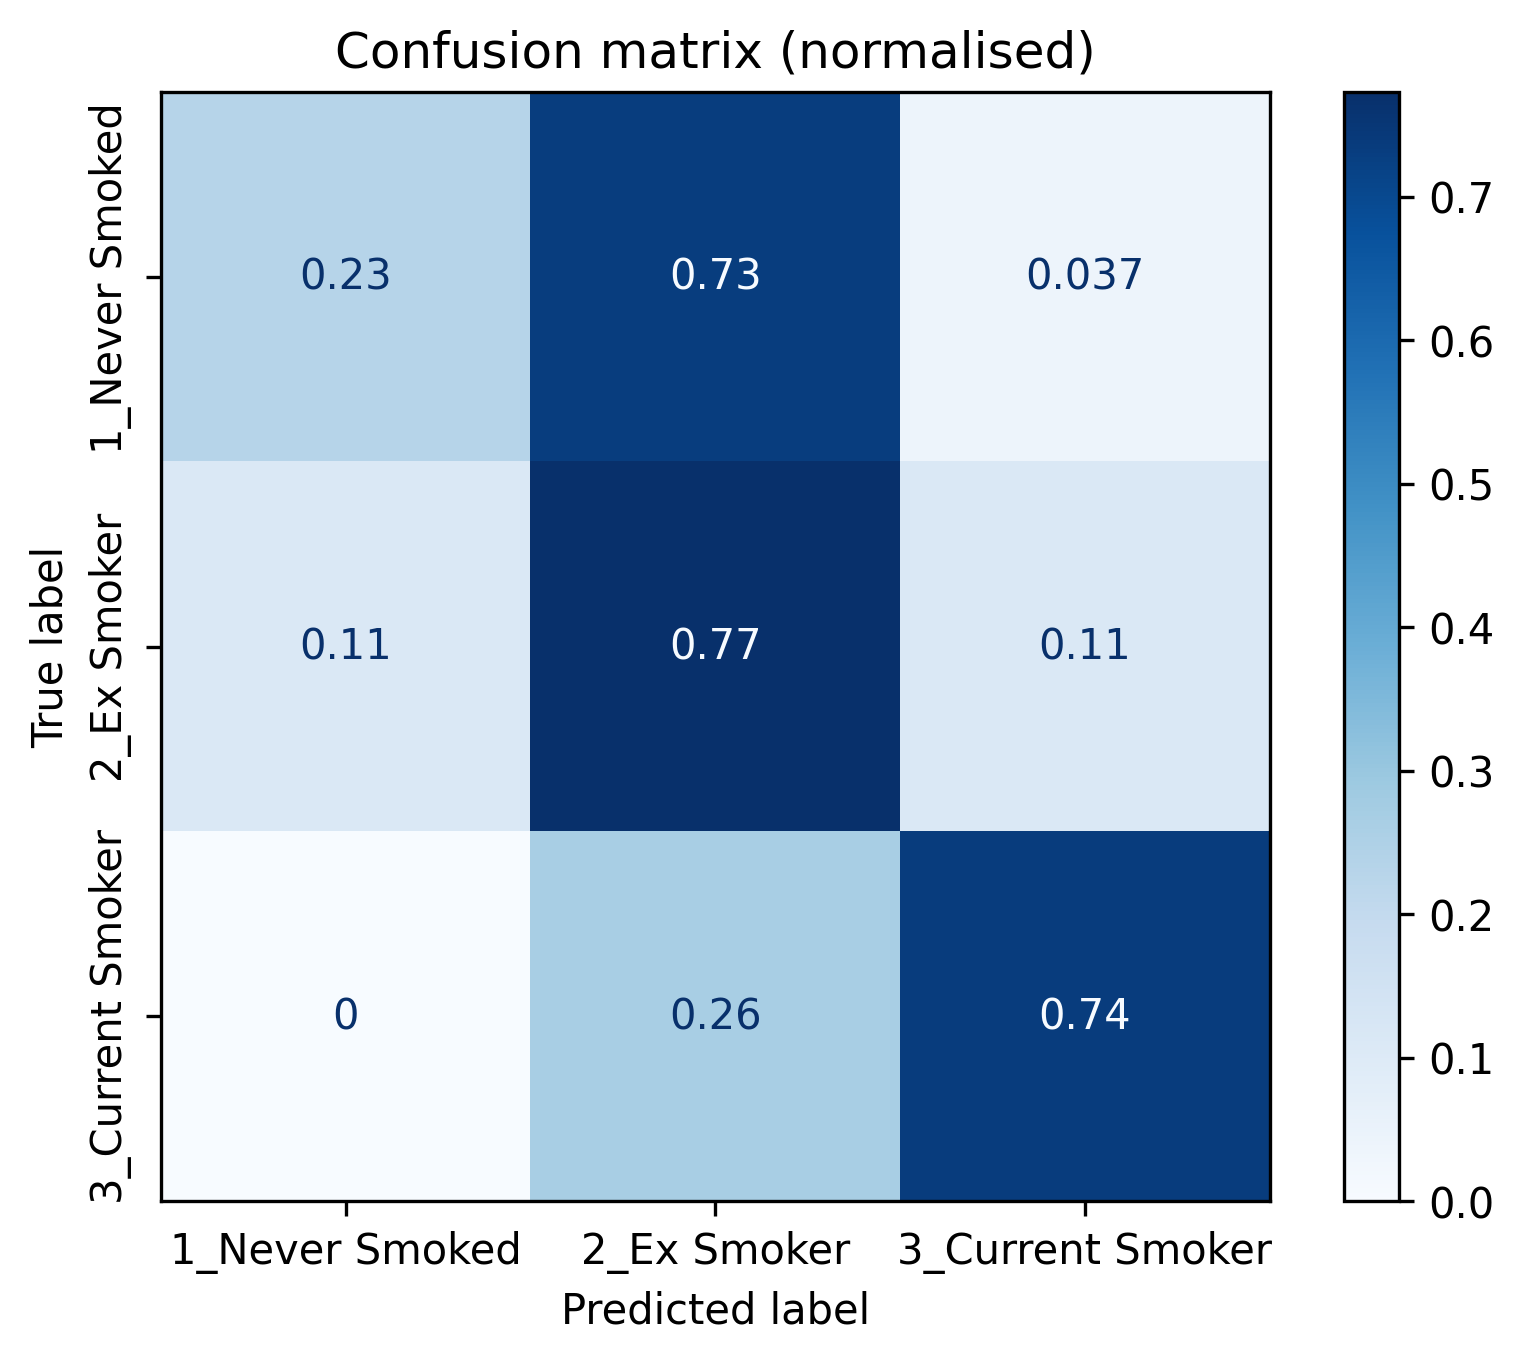
\includegraphics[width=\linewidth]{cohort2/female_only/test_confusion_matrix_normalised.png}
        \caption{Percentages}
    \end{subfigure}
    \caption[Confusion matrices (Cohort 2, female only)]{Confusion matrices (Cohort 2, female only)}
    \label{fig:female-only-confusion-matrix}
\end{figure}

\begin{figure}[p]
    \centering
    \begin{subfigure}{0.45\linewidth}
        \centering
        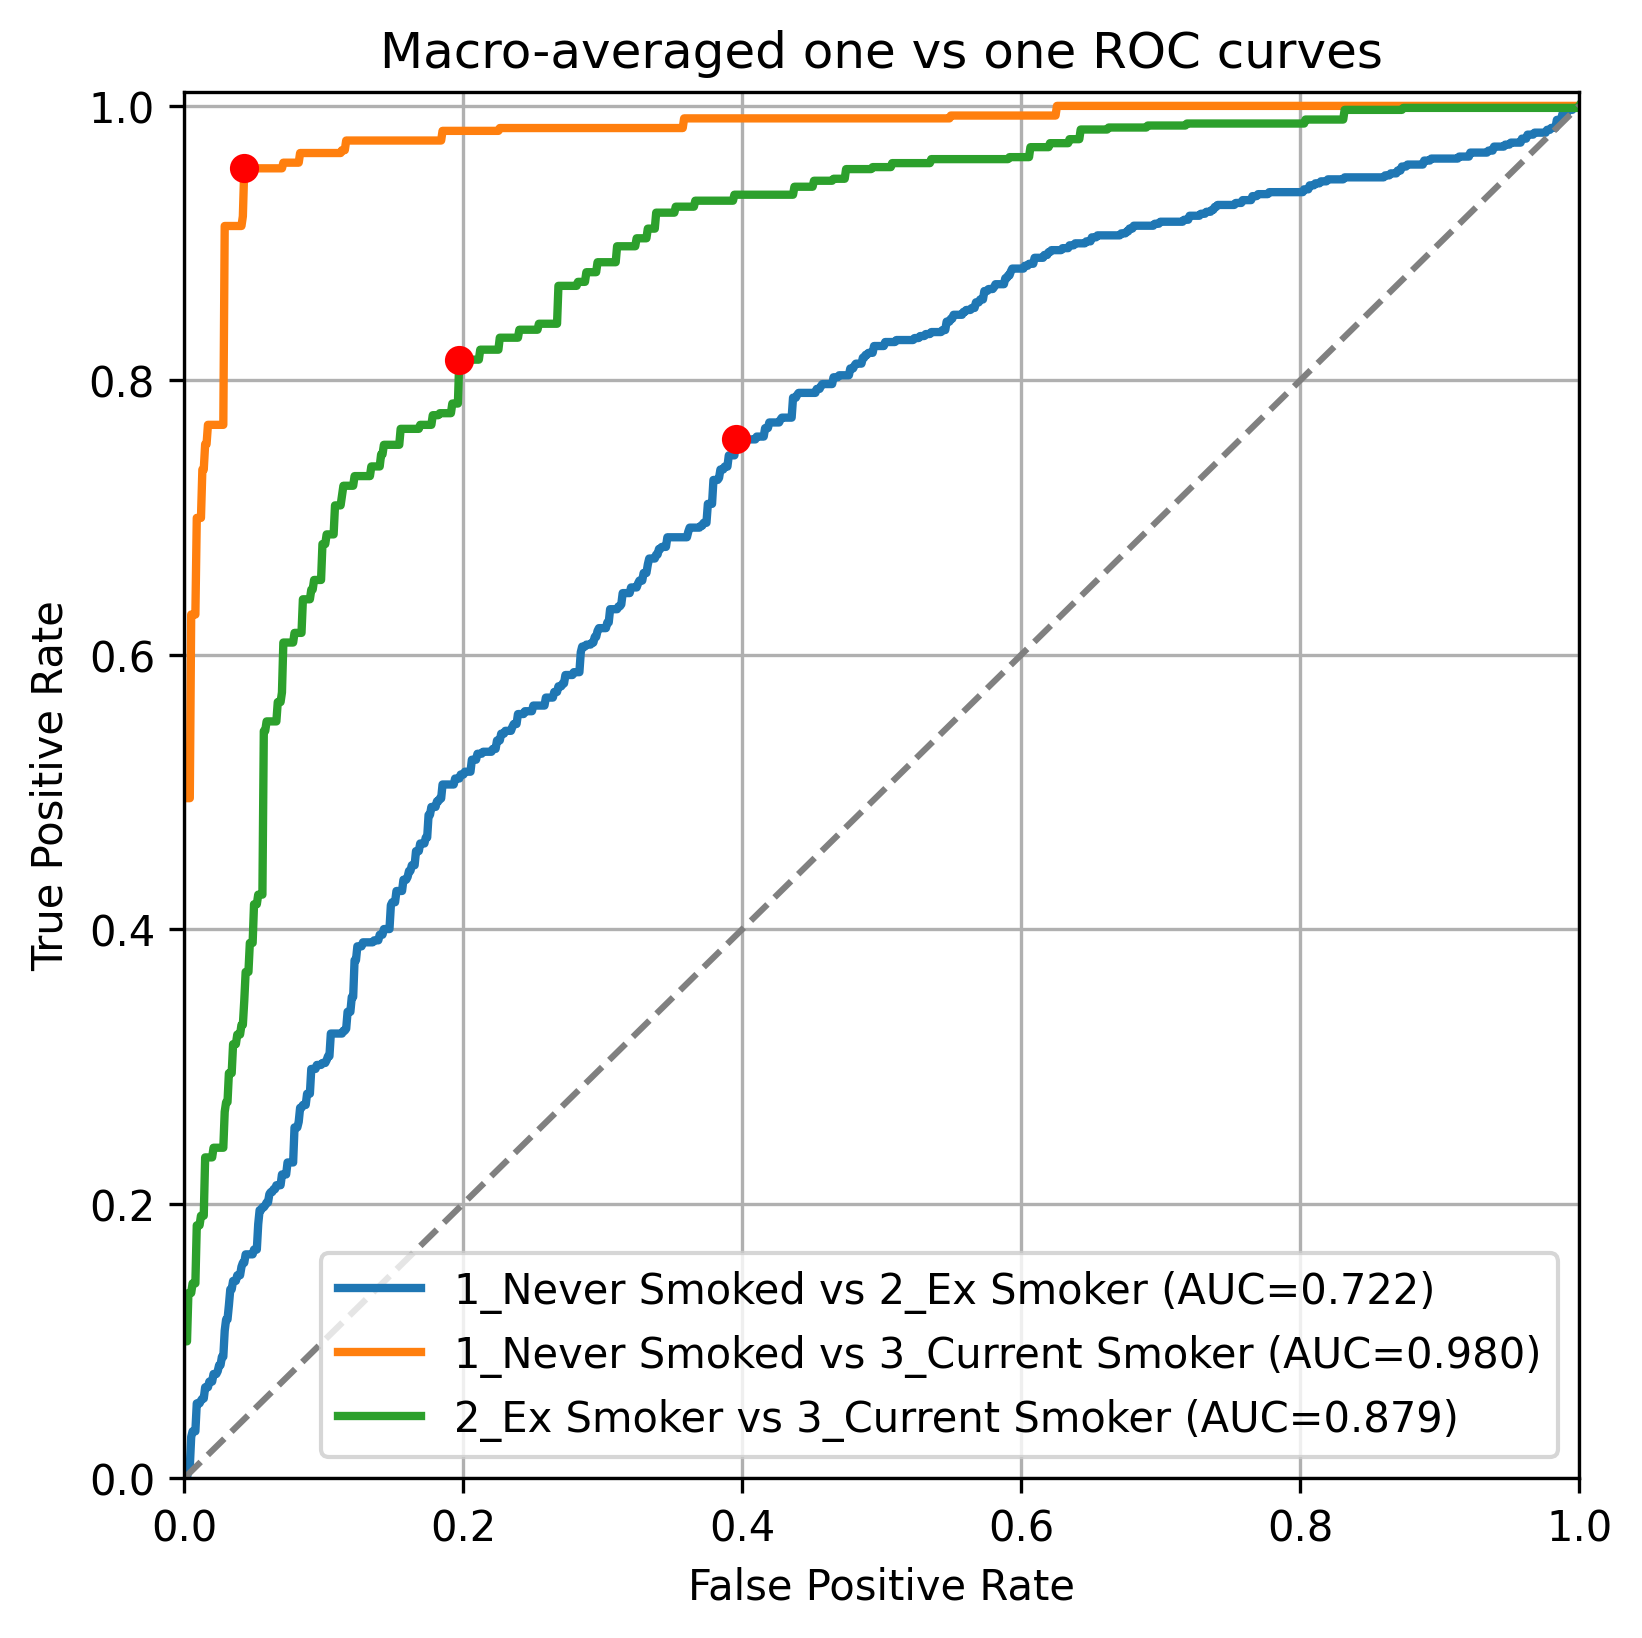
\includegraphics[width=\linewidth]{cohort2/male_only/test_macro_ovo_roc.png}
        \caption{Male only}
    \end{subfigure}
    \hspace{4mm}
    \begin{subfigure}{0.45\linewidth}
        \centering
        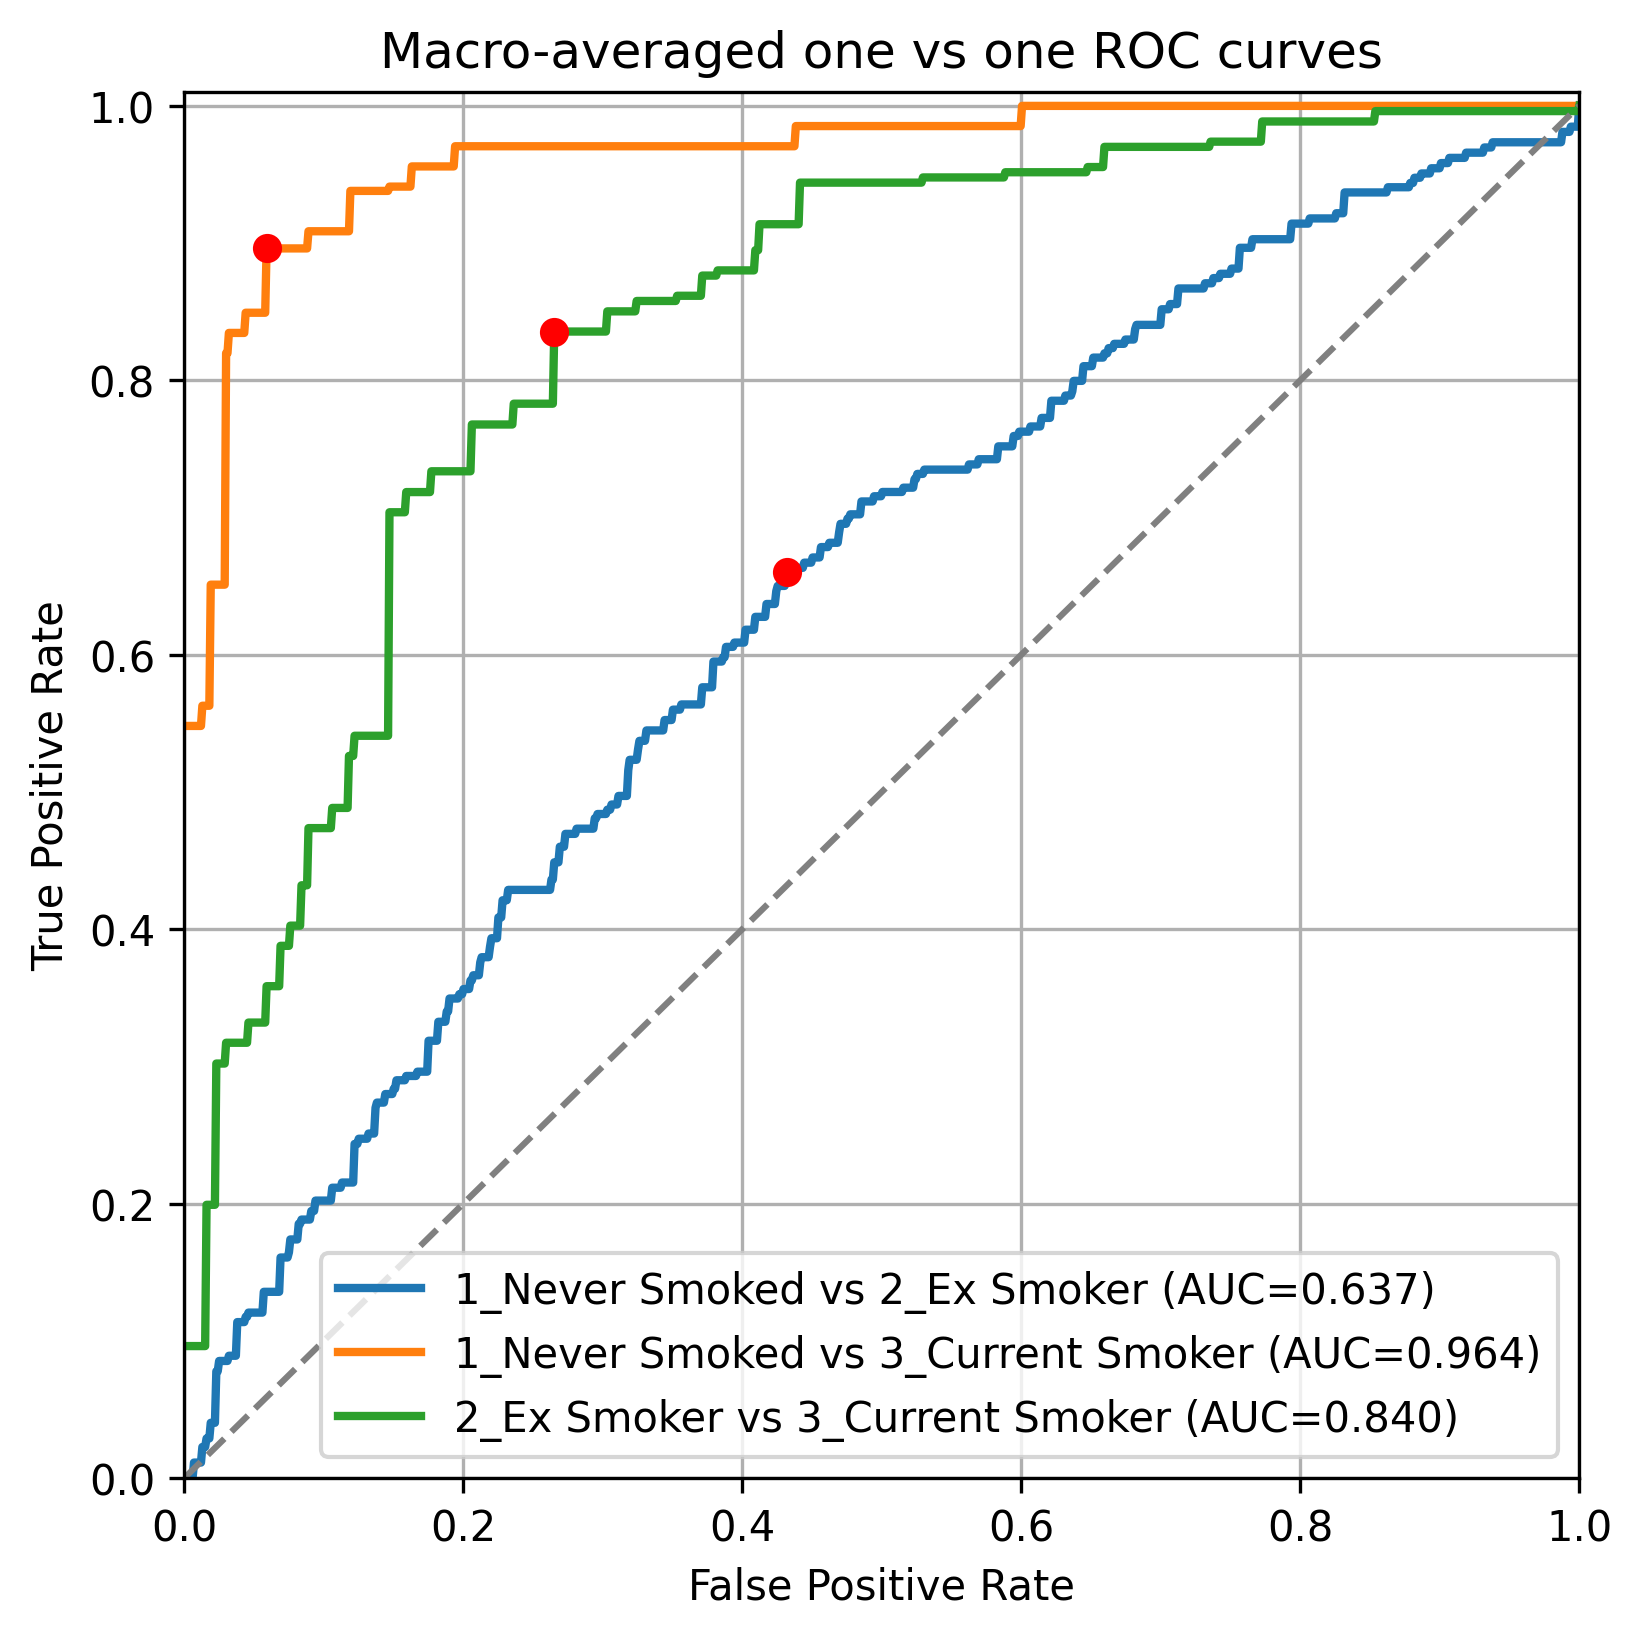
\includegraphics[width=\linewidth]{cohort2/female_only/test_macro_ovo_roc.png}
        \caption{Female only}
    \end{subfigure}
    \caption[Macro-averaged ROC curves (Cohort 2, separated by sex)]{Macro-averaged ROC curves (Cohort 2, separated by sex)}
    \label{fig:sex-sep-macro-rocs}
\end{figure}

ENSS was trained on Cohort 1, which only included male individuals. However, independent evaluation used Cohort 2, which contains both males and females. This raises the concern of sex being a potential confounding variable. This is especially relevant for smoking, as tobacco use is much higher in males than in females \cite{WHO2021Tobacco, higgins2015literature}. In order to assess this, evaluation was re-ran in Cohort 2 while separating for sex.

Classification performance on Cohort 2 males can be seen in Figure \ref{fig:male-only-confusion-matrix}, while classification performance on Cohort 2 females can be seen in Figure \ref{fig:female-only-confusion-matrix}. Performance for classifying ex-smokers and current-smokers appeared to be consistent, with \SI{78}{\percent} of male ex-smokers and \SI{77}{\percent} of female ex-smokers correctly classified, and \SI{73}{\percent} of male current-smokers and \SI{74}{\percent} of female current-smokers correctly classified. However, classification performance for never-smokers varied between males and females. \SI{73}{\percent} of female never-smokers were misclassified as ex-smokers, with \SI{23}{\percent} correctly classified, while \SI{54}{\percent} of male never-smokers were misclassified as ex-smokers, with \SI{45}{\percent} correctly classified. While classification of never-smokers was more accurate in males than females, performance was still poor in males, suggesting sex was only a partial confounding variable, with other factors leading to poor performance.

As before, the model's ability to separate classes was also evaluated. Macro-averaged OvO ROC curves for Cohort 2 males and Cohort 2 females can be seen in Figure \ref{fig:sex-sep-macro-rocs}. AUCs for these curves were similar across sexes.
ENSS achieved AUCs of: 0.980 on males and 0.964 on females for separating never-smokers from current-smokers, 0.879 on males and 0.840 on females for separating ex-smokers from current-smokers, and 0.772 on males and 0.637 on females for separating never-smokers from ex-smokers. Separation performance appeared to be consistent with the trend seen in classification, with the largest decrease in performance between sexes for never-smokers. As before, separating the cohort by sex only led to a minor increase in performance, suggesting sex was only a partial confounding variable.

\subsection{Comparison of ENSS to existing results (Cohort 2)} \label{sec:model-comparisons}

% \subsubsection{Benchmarking existing gold-standard models (Cohort 1 \& 2)} \label{sec:prior-benchmarks}
% \begin{enumerate}
%     \item Benchmark performance of externally derived gold standard models (DNAmPACKYRS and mCigarette) in both cohorts
%           \begin{itemize}
%               \item Benchmarking scores against self-reported smoking status
%               \item ROC diagrams
%               \item quick evaluation if predictive performance is comparable in both cohorts used in this study
%           \end{itemize}
% \end{enumerate}

\subsubsection{Comparison of CpG sites used in all 3 models} \label{sec:sites-comparison}

The intersections of the different sites used in DNAmPACKYRS and mCigarette with the never-, ex- and current-smoker class-specific predictors can be seen in Figure \ref{fig:cpg-intersection-external}. There was limited overlap between the CpG sites used in all three models. Only 11 sites were common to all three models. Per class-specific predictor, 11 sites were common to the never-smokers predictor, DNAmPACKYRS and mCigarette, 10 sites were common to the ex-smokers predictor, DNAmPACKYRS and mCigarette, and 10 sites were common to the current-smokers predictor, DNAmPACKYRS and mCigarette. However, only 14 CpG sites were common between DNAmPACKYRS and mCigarette, with 158 and 1241 CpG sites unique to those models, respectively. While there does not appear to be significant overlap between the features used in ENSS and either DNAmPACKYRS and mCigarette, neither was there significant overlap between the features used in DNAmPACKYRS and mCigarette, despite all three models being produced from datasets using the same \num{449521} CpG sites. Therefore, the intersection of (or lack thereof) ENSS with previous models appears to be consistent. This could be indicative of redundancy within the methylation signal, where different models can each select several different CpG sites to achieve the same effect.

\begin{figure}
    \centering
    \begin{subfigure}{0.49\linewidth}
        \centering
        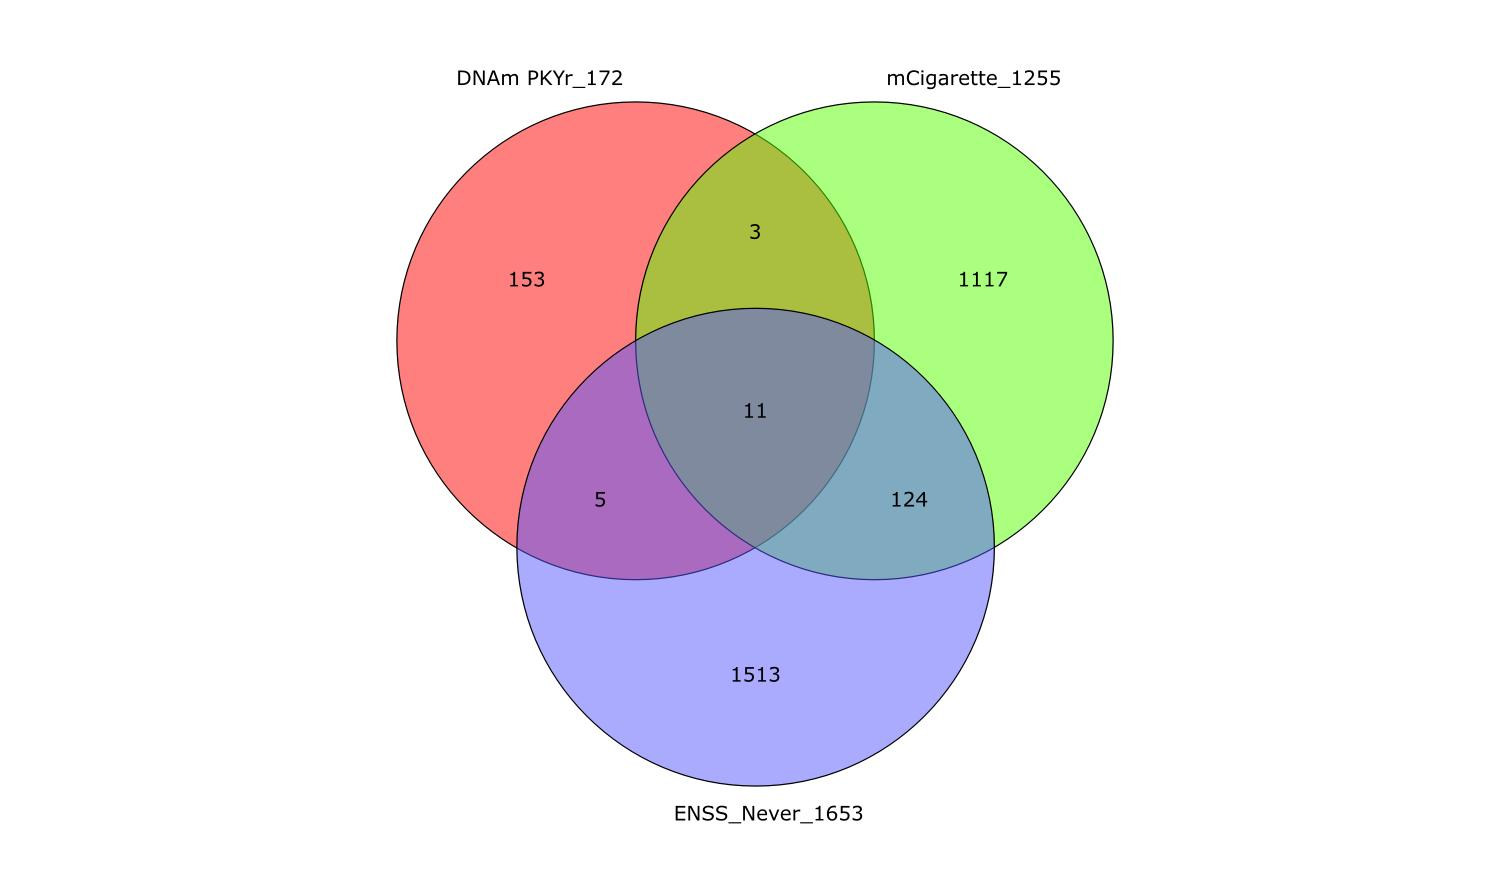
\includegraphics[width=\linewidth, trim=5cm 0cm 5cm 0cm, clip]{venn_diagrams/intersect_compare_never.jpg}
        % \caption[short]{title}
    \end{subfigure}
    \hfill
    \begin{subfigure}{0.49\linewidth}
        \centering
        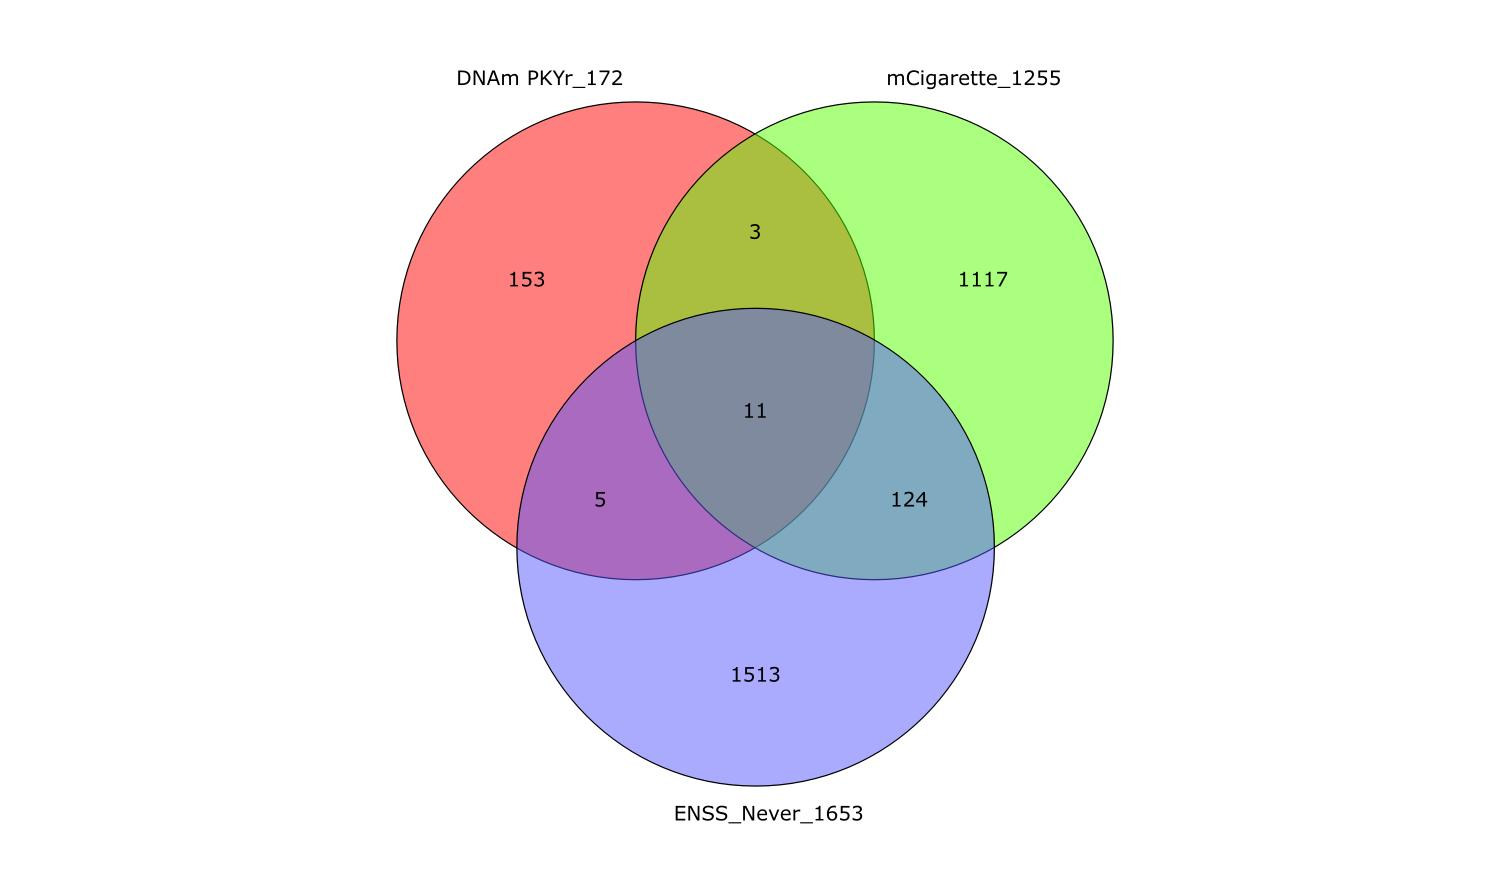
\includegraphics[width=\linewidth, trim=5cm 0cm 5cm 0cm, clip]{venn_diagrams/intersect_compare_never.jpg}
        % \caption[short]{title}
    \end{subfigure}

    \begin{subfigure}{0.49\linewidth}
        \centering
        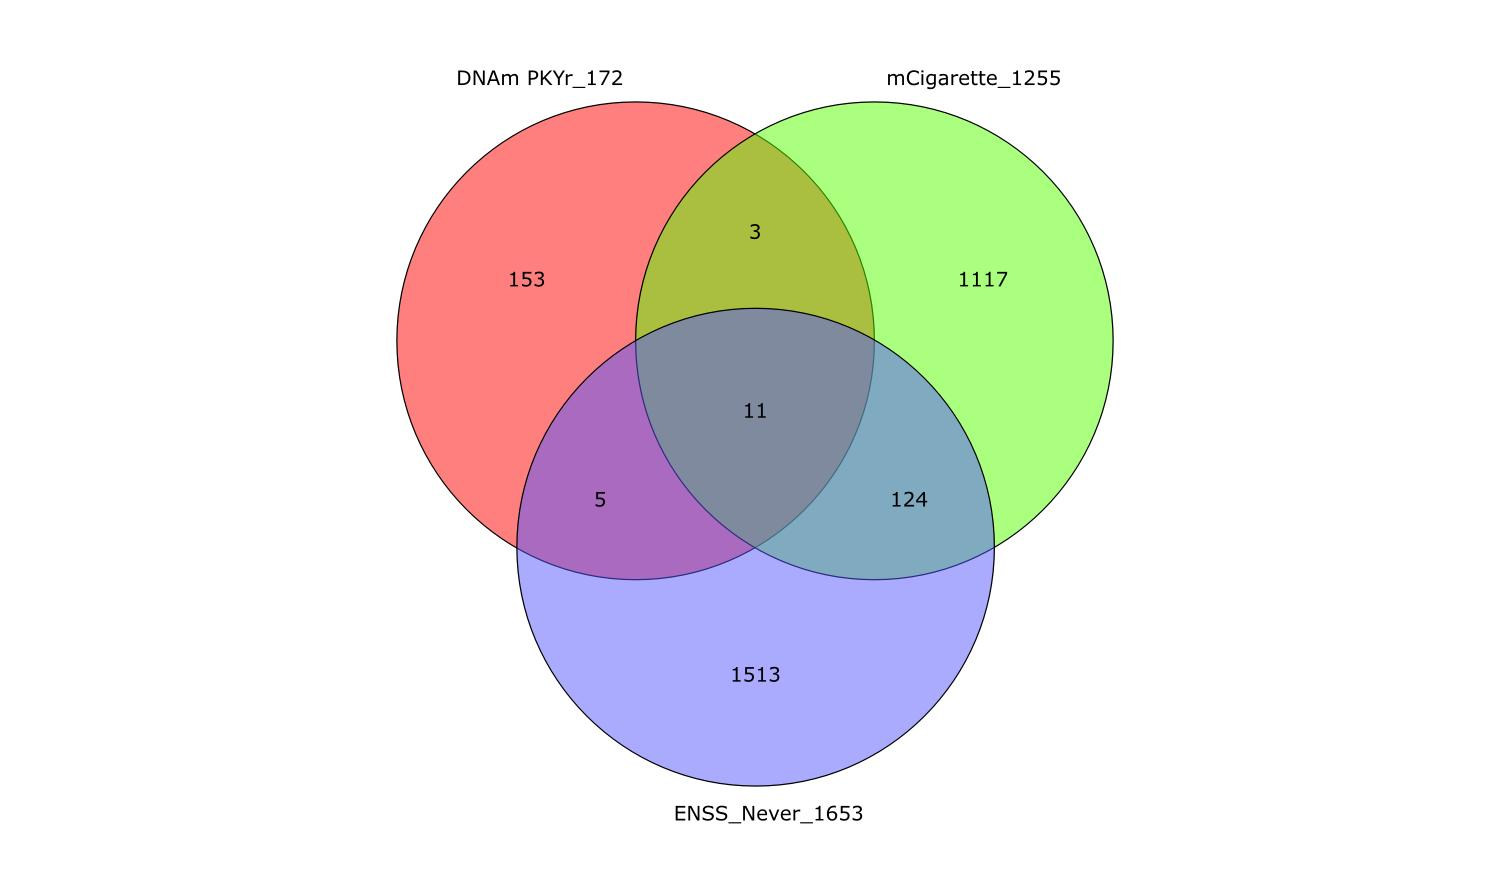
\includegraphics[width=\linewidth, trim=5cm 0cm 5cm 0cm, clip]{venn_diagrams/intersect_compare_never.jpg}
        % \caption[short]{title}
    \end{subfigure}
    \caption[Intersections of CpG sites with prior models]{Intersections of CpG sites with prior models}
    \label{fig:cpg-intersection-external}
\end{figure}


\begin{table}[b]
    \caption{Comparison of feature reduction steps} \label{table:sites-used}
    \begin{tabularx}{\textwidth}{X r r r r r r}
        \toprule
        \multirow{2}{*}{\textbf{Reduction step}} & \multirow{2}{*}{\textbf{DNAmPY}} & \multirow{2}{*}{\textbf{mCigarette}} & \multicolumn{3}{c}{\textbf{ENSS}} & \multirow{2}{*}{\textbf{Linear}}                               \\
        \cmidrule(lr){4-6}
                                                 &                                  &                                      & Nvr.                              & Ex                               & Curr.        &              \\
        \midrule
        Starting CpG sites                       & \num{450161}                     & \num{449521}                         & \num{449521}                      & \num{449521}                     & \num{449521} & \num{449521} \\
        \addlinespace
        Post statistical test                    & N/A                              & \num{187600}                         & \num{3122}                        & \num{3122}                       & \num{3122}   & \num{3122}   \\
        \addlinespace
        Post ML regularisation                   & \num{172}                        & \num{1255}                           & \num{1653}                        & \num{1627}                       & \num{1514}   & \num{57}     \\
        \bottomrule
    \end{tabularx}
\end{table}

The effects of regularisation on the model were not consistent with prior results. Comparisons of feature reduction steps can be seen in Table \ref{table:sites-used}. Regularisation in the training of DNAmPACKYRS selected 172 features out of \num{450161}, while regularisation in the training of mCigarette selected \num{1255} features out of \num{187600}. However, the three class-specific predictors of ENSS each selected 1653, 1627 and 1514 features out of 3122, respectively. While the hyperparameter choices for DNAmPACKYRS are not publicly available, mCigarette used a choice of \(\alpha = 0.012577\) and \(\lambda = 0.5\), whereas ENSS was trained using \(\alpha = 0.2\) and \(\lambda = 0.85\). Therefore, ENSS was trained using stronger regularisation than mCigarette yet proportionally selected more features, suggesting the model overfitted the training data. An Elastic Net linear regression model was trained as a benchmark to evaluate this hypothesis. Regularisation in the training of this linear benchmark selected 57 features out of 3122, which is in line with the regularisation seen in DNAmPACKYRS and mCigarette.

\subsubsection{Evaluating performance with ROC comparisons}

\begin{figure}[p]
    \centering
    \begin{subfigure}{0.48\linewidth}
        \centering
        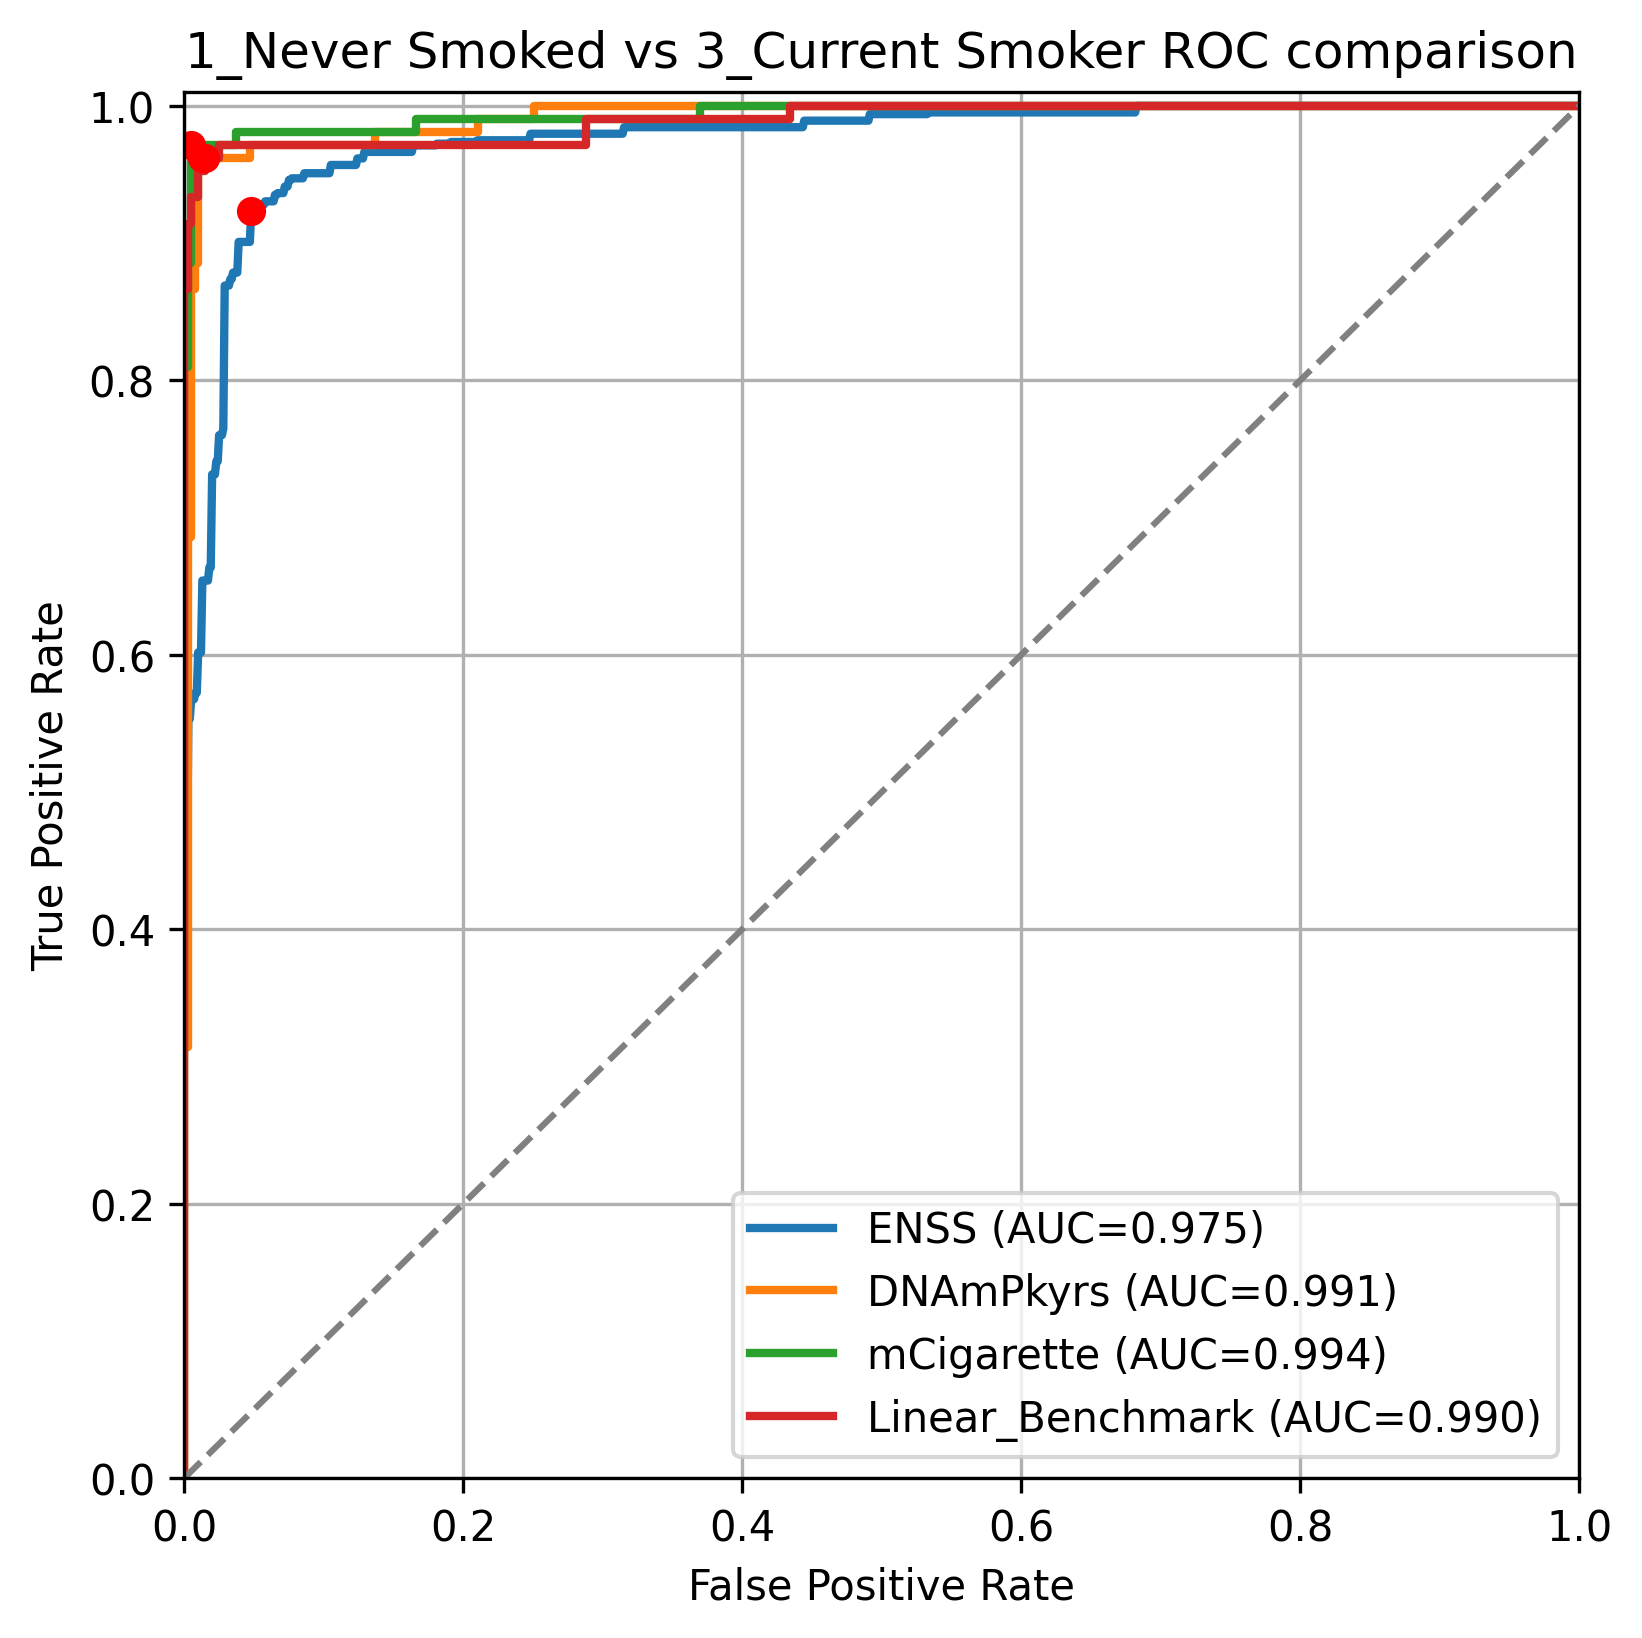
\includegraphics[width=\linewidth]{comparison_1v3.png}
    \end{subfigure}
    \hfill
    \begin{subfigure}{0.48\linewidth}
        \centering
        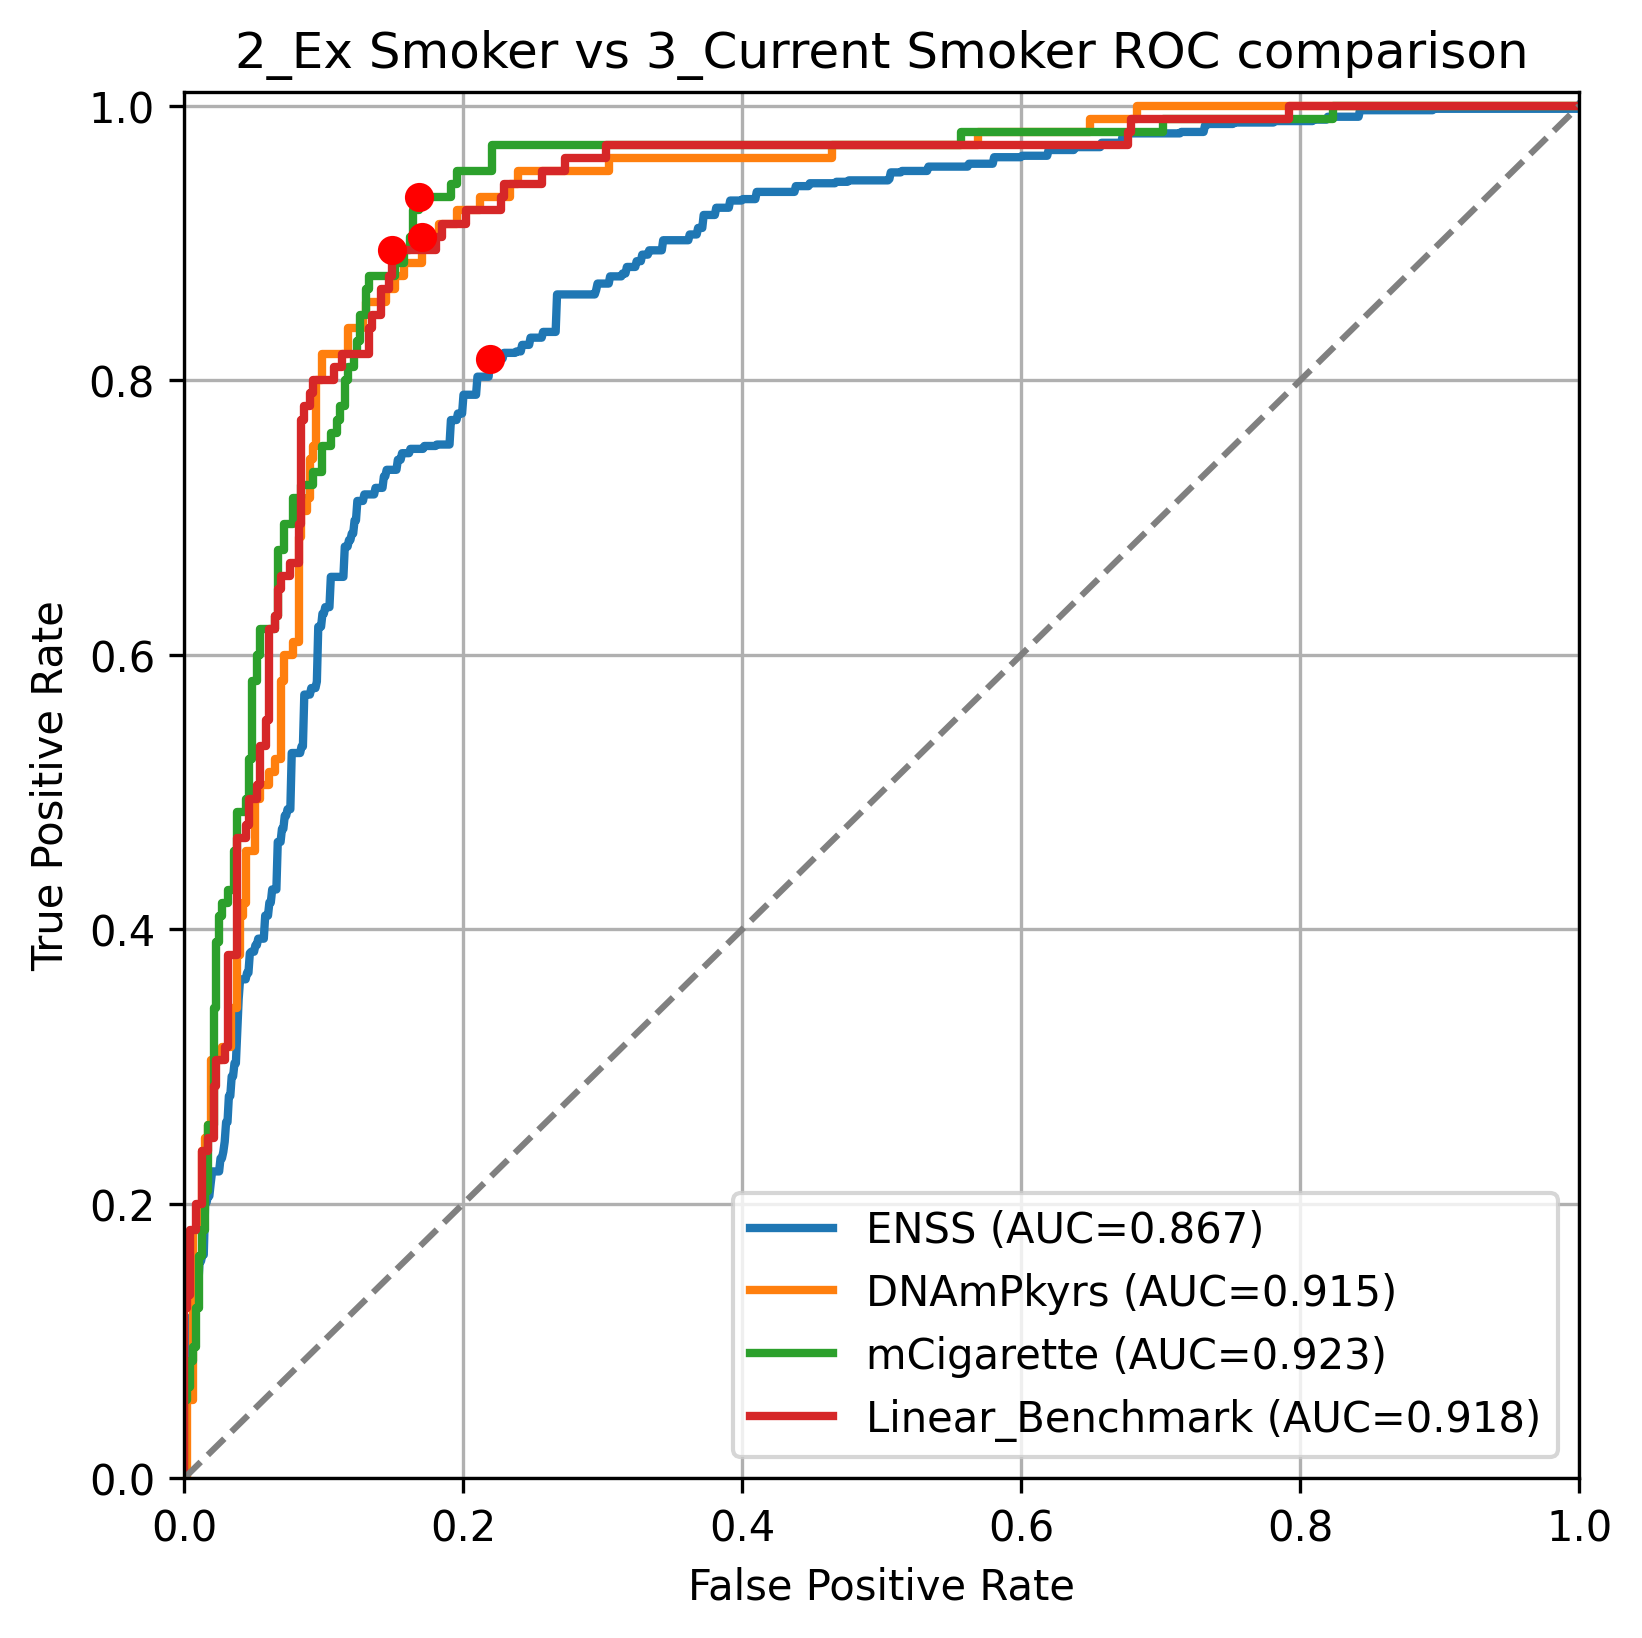
\includegraphics[width=\linewidth]{comparison_2v3.png}
    \end{subfigure}
    \begin{subfigure}{0.48\linewidth}
        \centering
        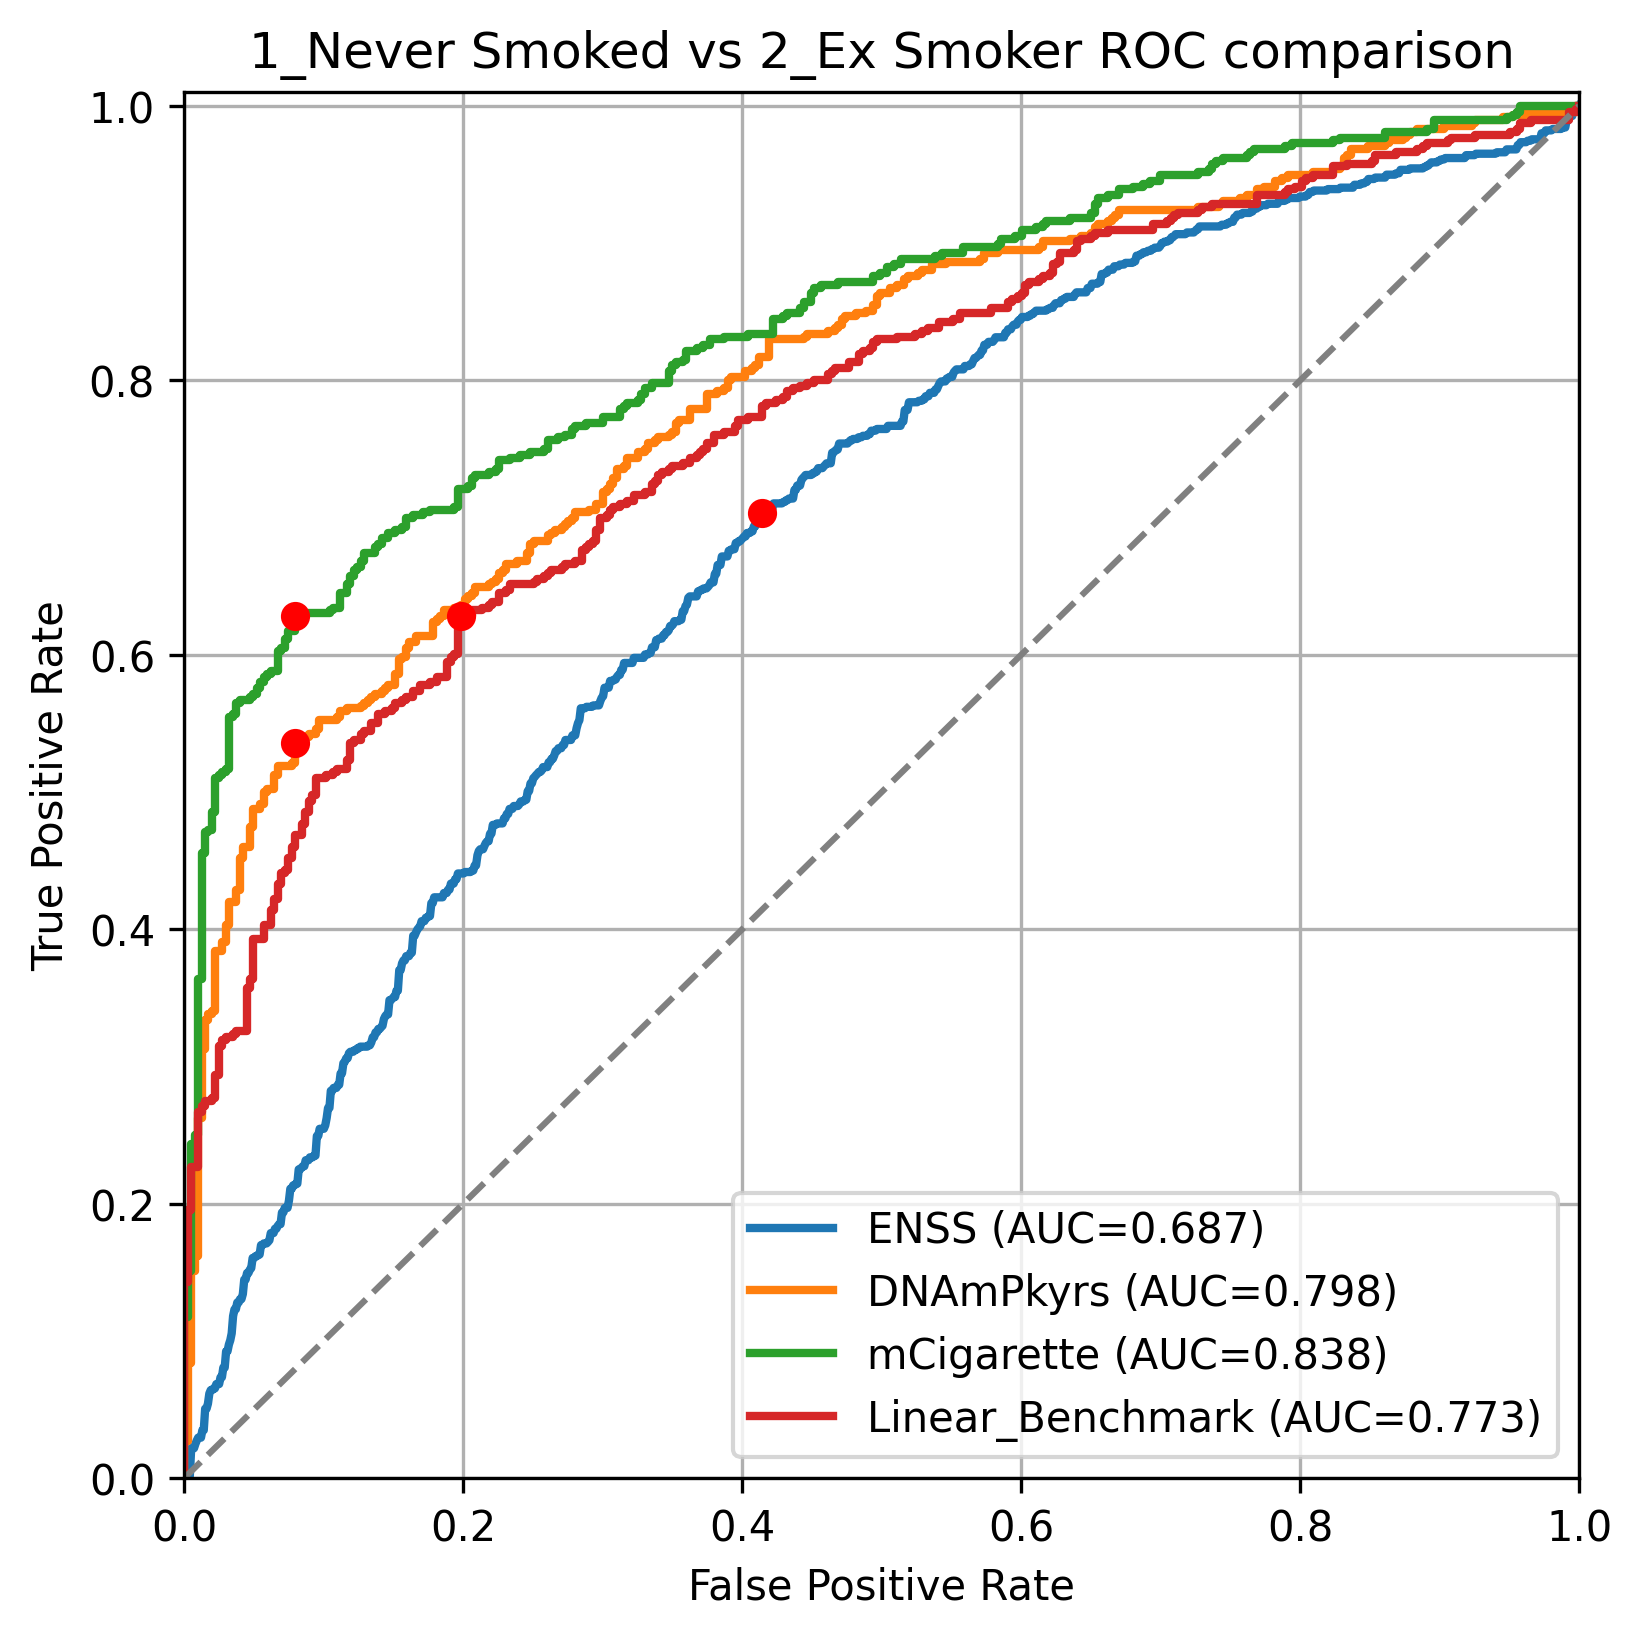
\includegraphics[width=\linewidth]{comparison_1v2.png}
    \end{subfigure}
    \caption[Comparison of ROC curves with prior results]{Comparison of ROC curves with prior results. }
    \label{fig:comparison-rocs}
\end{figure}

To avoid discovery bias associated with the training cohort, model comparisons were only evaluated using Cohort 2. OvO ROC curves comparing Elastic Net Smoking-Status, DNAmPACKYRS and mCigarette can be seen in Figure \ref{fig:comparison-rocs}. All three models achieved excellent performance separating never-smokers from current-smokers. Namely, ENSS achieved an ROC-AUC of 0.971, DNAmPACKYRS achieved an ROC-AUC of 0.991 and mCigarette achieved an ROC-AUC of 0.994. Both DNAmPACKYRS and mCigarette achieved excellent performance separating ex-smokers from current-smokers, with ROC-AUCs of 0.915 and 0.923, respectively, while Elastic Net Smoking-Status achieved good performance, with an ROC-AUC of 0.859. For separating never-smokers from ex-smokers, mCigarette achieved good performance with an ROC-AUC of 0.838, DNAmPACKYRS achieved acceptable performance with an ROC-AUC of 0.798, while ENSS achieved poor performance with an ROC-AUC of 0.686. A summary of these AUCs can be seen in Table \ref{table:auc-comparison}.

Comparing ENSS to prior results shows worse performance in the independent cohort, indicative of overfitting. In order to diagnose this, a simpler linear model was trained to benchmark the utility of the training dataset. OvO ROC curves of this model can be seen in Figure \ref{fig:comparison-rocs}. The linear benchmark achieved ROC-AUCs of: 0.990 for separating never-smokers from current-smokers, 0.918 for separating ex-smokers from current-smokers, and 0.773 for separating never-smokers from ex-smokers. This performance was similar to that of DNAmPACKYRS and mCigarette, and outperformed ENSS. Comparing linear to logistic models, both internally and externally derived linear models outperformed the internally derived logistic model. Moreover, the linear benchmark was not tuned or optimised, and used the same hyperparameters as the logistic model. This result suggests that the poor regularisation of ENSS was due to the model itself, rather than the quality of the training dataset.

\begin{table}[p]
    \caption{Summary of model ROC-AUCs in Cohort 2 independent test set} \label{table:auc-comparison}
    \begin{tabularx}{\textwidth}{X >{\centering\arraybackslash}X >{\centering\arraybackslash}X >{\centering\arraybackslash}X}
        \toprule
        \multirow{2}{*}{\textbf{Model}} & \multicolumn{3}{c}{\textbf{AUC}}                               \\
        \cmidrule(lr){2-4}
                                        & Never vs Current                 & Ex vs Current & Never vs Ex \\
        \midrule
        DNAmPACKYRS                     & \num{0.911}                      & \num{0.915}   & \num{0.798} \\
        \addlinespace
        mCigarette                      & \num{0.994}                      & \num{0.923}   & \num{0.838} \\
        \addlinespace
        ENSS                            & \num{0.971}                      & \num{0.859}   & \num{0.686} \\
        \addlinespace
        Linear benchmark                & \num{0.990}                      & \num{0.918}   & \num{0.773} \\
        \bottomrule
    \end{tabularx}
\end{table}

\section{Discussion}

\begin{table}[b]
    \caption{Training dataset comparisons with prior studies} \label{table:dataset-compare-external}
    \begin{tabularx}{\textwidth}{X >{\raggedleft\arraybackslash}X >{\raggedleft\arraybackslash}X >{\raggedleft\arraybackslash}X}
        \toprule
        \textbf{Measure} & \textbf{Cohort 1 - Train}     & \textbf{FHS}                  & \textbf{GS}                    \\
        % \addlinespace
        \midrule
        \multicolumn{4}{c}{\textbf{Class balance}}                                                                        \\
        \midrule
        Num. individuals & \num{848}                     & \num{1731}                    & \num{17865}                    \\
        \addlinespace
        Never-Smokers    & \num{211} (\SI{25}{\percent}) & \num{710} (\SI{41}{\percent}) & \num{3277} (\SI{18}{\percent}) \\
        \addlinespace
        Ex-Smokers       & \num{539} (\SI{63}{\percent}) & \num{883} (\SI{51}{\percent}) & \num{9414} (\SI{53}{\percent}) \\
        \addlinespace
        Current-Smokers  & \num{98} (\SI{12}{\percent})  & \num{138} (\SI{8}{\percent})  & \num{5174} (\SI{29}{\percent}) \\
        % \addlinespace
        \midrule
        \multicolumn{4}{c}{\textbf{Cohort distribution}}                                                                  \\
        \midrule
        Percentage male  & \SI{100}{\percent}            & \SI{46}{\percent}             & \SI{59.1}{\percent}            \\
        Mean age (years) & \num{72}                      & \num{66}                      & \num{47.6}                     \\
        \bottomrule
    \end{tabularx}
\end{table}

While ENSS achieved excellent discrimination in the hold-out testing dataset (ROC-AUCs: 0.977, 0.941, 0.909), performance ranged from excellent to poor in the independent testing dataset (ROC-AUCs: 0.971, 0.859, 0.686). When compared the current gold-standard smoking models DNAmPACKYRS (ROC-AUCs: 0.991, 0.915, 0.798) and mCigarette (ROC-AUCs: 0.994, 0.923, 0.838), we can see ENSS achieved similar performance separating never-smokers from current-smokers, but worse performance separating ex-smokers from current-smokers and never-smokers from ex-smokers. All three of these models were developed using a similar selection of CpG sites (intersection of the 450k and EPIC arrays), and took similar approaches with feature selection, cross validation and training. Therefore, the most likely cause of the discrepancies seen in performance are the differences between the training datasets used, namely the distribution of sex and sample size. While ENSS was produced from a dataset only containing males, the DNAmPACKYRS and mCigarette scores were not, and had both males and females present in their training data (see Table \ref{table:dataset-compare-external}). However, separating males from females in the independent testing dataset resulted in only an incremental gain in performance, suggesting sex was not a substantial confounding variable. In terms of sample size, the training dataset for ENSS only contained 848 individuals, compared to \num{1731} (FHS) for DNAmPACKYRS and \num{17865} (GS) for mCigarette (see Table \ref{table:dataset-compare-external}). Moreover, ENSS was significantly more complex than DNAmPACKYRS or mCigarette, using more CpG sites (see Figure \ref{fig:cpg-intersection-external} and Table \ref{table:sites-used}). Producing a simpler model (Elastic Net linear regression) on the same training dataset resulted in performance comparable to DNAmPACKYRS and mCigarette (ROC-AUCs: 0.990, 0.918, 0.773). This suggests that the additional complexity of the logistic regression model is promoting overfitting, which is consistent with machine learning theory \cite{bishop2006pattern}. An increased training sample size can reduce overfitting \cite{bishop2006pattern}, which could explain the increased performance of DNAmPACKYRS and mCigarette in the independent dataset. Similarly, this could potentially resolve overfitting issues of ENSS. The other conventional approach to overfitting is increasing regularisation strength \cite{buhlmann2011statistics}. However, it should be noted that this did not work in practice as ENSS was trained with stronger regularisation than mCigarette, yet proportionally selected more features to be used in the final model. One explanation for overfitting could be due to the fact that the sample complexity for logistic regression grows with the number of irrelevant features \cite{ng2004feature}. This suggests that no amount of hyperparameter tuning would have improved model performance in the independent test dataset, without sufficient sample size in the training dataset.

\subsection{Limitations of this work} \label{sec:limitations}
There were several limitations associated with this work. Firstly, the labels for supervised learning used self-reported data. Self-reported data is prone to inaccuracy (see
\ref{sec:srss}), and therefore, potentially introduces bias into a trained model. In training, an incorrectly labelled example could lead to gradient updates which are not related to the true relationship between training data and model output. In evaluation, an incorrectly labelled example could lead to a correct model prediction being identified as erroneous, skewing the perception of the model's accuracy. This limitation is not unique to this work, and would be expected to be present for the DNAmPACKYRS and mCigarette scores as well.

As discussed, the trained logistic regression model (ENSS) overfits the training data. While traditional machine learning evaluation showed excellent performance separating all classes, independent evaluation representative of practical applications showed ENSS overfitting, with class separation ranging from excellent to poor. However, a linear regression model (linear benchmark) trained on the same dataset outperformed the logistic approach. We hypothesised that this was largely due to differences in model complexity, and more training data would be required when using a logistic approach. However, even with this hypothesis verified, this means the required sample size limits the utility of our proposed method. Large sample sizes are not always available, especially for epigenetic data. Therefore, even with overfitting addressed, the method proposed in this work maybe be unsuitable for some applications.

\subsection{Future Directions}
Recent work has shown promise integrating principal component analysis (PCA) into Elastic Net model training \cite{higgins2022computational}. Using only a single additional step, PC-based Elastic Net showed improvements in reliability and performance, due to reducing the effect of noise present in the dataset. Moreover, using Elastic Net models trained on principal components (rather than CpG sites) has benefits for interpretability and regularisation. While this method has shown improvements for DNAm-based aging clocks, little work has been done to evaluate the benefits for DNAm-based smoking scores. Moreover, improvements associated with regularisation and noise could help reduce the overfitting problem present with the method proposed in this work.

This worked aimed to improve class separation by reframing the problem of modelling lifetime smoking exposure as a classification task rather than a regression task. To achieve this, we adapted the existing gold-standard techniques, which use linear regression, into logistic regression algorithms. However, there are other choices of classification algorithms to explore. Decision trees are one such example that show promise. Decision trees are relatively simple models, and therefore could perform well with smaller training datasets, addressing a limitation of ENSS. Moreover, decision tree training requires iteratively selecting features in training, which could leverage the existing Kruskal-Wallis feature selection used in this method. Additionally, ensemble methods such as random forests or gradient boosting (e.g. XGBoost) provide options for increased accuracy, however, at the cost of interpretability.

\section{Footnotes}

\subsection{Ethics Statement}
All participants gave written informed consent, and the study was approved by the national ethics committee. Data was anonymised and only age, biological sex and self-reported smoking values were extracted for comparison with matching whole blood DNA methylation values.

\subsection{Acknowledgements}

\addcontentsline{toc}{section}{References}
\printbibliography

\end{document}